\documentclass[12pt]{ucsd}
% mathptmx is a Times Roman look-alike (don't use the times package)
% It isn't clear if Times is required. The OGS manual lists several
% "standard fonts" but never says they need to be used.
\usepackage{mathptmx}
\usepackage[NoDate]{currvita}
\usepackage{array}
\usepackage{tabularx}
\usepackage{booktabs}
\usepackage{subfig}
\usepackage{ragged2e}
\usepackage{microtype}
\usepackage[breaklinks=true,pdfborder={0 0 0}]{hyperref}
\usepackage{graphicx}
\AtBeginDocument{%
	\settowidth\cvlabelwidth{\cvlabelfont 0000--0000}%
}

% OGS recommends increasing the margins slightly.
\increasemargins{.1in}

% These are just for testing/examples, delete them
\usepackage{trace}
%\usepackage{showframe} % This package was just to see page margins
\usepackage[english]{babel}
\usepackage{blindtext}
\overfullrule5pt
% ---
% Reference for quotes
\def\signed #1{{\leavevmode\unskip\nobreak\hfil\penalty50\hskip2em
  \hbox{}\nobreak\hfil(#1)%
  \parfillskip=0pt \finalhyphendemerits=0 \endgraf}}
% Custom quote environment
\newsavebox\mybox
\newenvironment{aquote}[1]
  {\savebox\mybox{#1}\begin{quote}}
  {\signed{\usebox\mybox}\end{quote}}
% ---

% Required information
\title{This is the Title of My Dissertation}
\author{Jonathan Kasuke Guiang}
\degree{Physics}{Doctor of Philosophy}
% Each member of the committee should be listed as Professor Foo Bar.
% If Professor is not the correct title for one, then titles should be
% omitted entirely.
\chair{Professor Frank W\"urthwein}
\cochair{Professor Avi Yagil} % Optional
% Your committee members (other than the chairs) must be in alphabetical order
\committee{Professor Sekhar Chivukula}
\committee{Professor Albert Hsiao}
\committee{Professor Arun Kumar}
\committee{Professor Michael Norman}
\degreeyear{2024}

% Start the document
\begin{document}
% Begin with frontmatter and so forth
\frontmatter
\maketitle
\makecopyright
\makesignature

% --- Dedication ---
\begin{dedication}
\setsinglespacing
\parindent0pt\parskip\baselineskip
\begin{center}
This dissertation is dedicated to my wife Rosemary and the future we are building together; 
to my parents, Orlando and Cynthia Guiang, and my sister, Christina Guiang; 
to grandpa and grandma, John and Tsuneko Hashiguchi; 
to abuelo and abuela, Rufino and Aurelia Guiang; 
to the thousands of miles traveled, centuries of hardship endured, decades of triumph celebrated, and many wonderous years yet to come. 
I love you all more than words can express.
\end{center}
\end{dedication}


% --- Epigraph ---
\begin{epigraph}
\vskip0pt plus.5fil
\setsinglespacing

\begin{epiquote}{William Blake, Auguries of Innocence, 1863}
    To see a World in a Grain of Sand \\
    And a Heaven in a Wild Flower \\
    Hold Infinity in the palm of your hand \\
    And Eternity in an hour
\end{epiquote}

\begin{epiquote}{James Joyce, interview with Arthur Power, 1921}
    In the particular is contained the universal.
\end{epiquote}

\begin{epiquote}{James Baldwin, The Paris Review, 1984}
    Talent is insignificant. \\
    I know a lot of talented ruins. \\
    Beyond talent lie all \\
    the usual words: discipline, love, luck, \\ 
    but, most of all, endurance.
\end{epiquote}

\end{epigraph}


% Next comes the table of contents, list of figures, list of tables,
% etc. If you have code listings, you can use \listoflistings (or
% \lstlistoflistings) to have it be produced here as well. Same with
% \listofalgorithms.
\tableofcontents
\listoffigures
\listoftables

% --- Preface ---
\begin{preface}
Almost nothing is said in the manual about the preface. There is no
indication about how it is to be typeset. Given that, one is forced to
simply typeset it and hope it is accepted. It is, however, optional
and may be omitted.
\end{preface}


% --- Acknowledgements ---
\begin{acknowledgements}
Recorded in this dissertation, in great detail, are my contributions to a grand scientific enterprise. 
What is not documented, however, are the struggles, doubts, heartache, frustrations, and so much more that lie beyond the histograms, tables, and physics prose. 
Through each of these challenges, I am fortunate to have been surrounded by incredible people who ran beside me in the best of times, and dragged me along in the worst. 
Please find below my best attempt at thanking them, in mere sentences, for making all of this---and all that is to come---possible. 

Foremost, I owe boundless thanks to my incredible family. 
First, to Mom and Dad, thank you for raising me in a home full of love and imagination and for all of your work and sacrifice upon which my life, career, and now this dissertation have been built upon. 
And to Christina, my big sister: thank you for your strength and courage, for all of our memories growing up together (except, perhaps, those that ended with my injury), and for inspiring me to be bold. 
I am also fortunate to have spent a great deal of time with my grandparents, John and Tsuneko Hashiguchi---thank you, grandma and grandpa, for teaching me to be good and honest and for showing me how to persevere. 
Amidst all of my ``found'' family---family by bond, not blood---I must, most of all, thank my uncle, John Sanders: thank you for putting up with your briny nickname, for every phone call, for your humor (even when it is at my expense), and for helping me at every stage of my career. 
Finally, to my wife Rosemary, who has brightened my life in every way: thank you for your kindness and compassion, for everything that you are, I love you more than anything. 
I hope that today and on every day after, I can make you all proud.

I am equally grateful for the many mentors I have had in my relatively short academic career, organized here by the institution at which we met. 
Starting with UCSD, I thank Prof. Frank W\"urthwein, my advisor, who believed in me, guided me through all of my achievements, and flew me around the world---thank you, Frank, for everything. 
And to Prof. Avi Yagil, who served as my co-advisor: thank you for challenging, uplifting, and educating me. 
I also owe many thanks to Prof. Philip Chang who, in many ways, was also my co-advisor. 
For hours of conversation via Zoom and over 130\,000 Skype messages, for even more hours of physics and C++ lessons, and for your nearly endless patience: thank you, Philip. 
Next, from my alma mater, UCSB, I am ever indebted to Prof. Claudio Campagnari for taking me in and completely altering the course of my life. 
Claudio gave me purpose during what was, probably unbeknownst to him, a very difficult time for me personally---thank you, Claudio; without you, this dissertation simply would not exist. 
Also, Claudio's former students and postdocs were my first and most formative mentors. 
Thanks, in particular, to Dr. Nick Amin for teaching me everything I know. 
Thanks also Dr. Bennett Marsh, who mentored me across multiple projects---I am a better leader, person, and scientist thanks to Nick and Bennett. 
And to Prof. Indara Suarez, who welcomed me into particle physics and pushed me to meet my true potential: thank you for the high-octane tour of Boston in your Mustang, your thoughtful mentorship, and your constant support. 

I must also thank all of the members, past and present, of the illustrious ``Surf n' Turf'' (SNT) empire, whose dominion stretches far across the western world. 
It has been a privilege to serve as your Data Librarian, and I am deeply grateful to each of you, though, unfortunately, I do not have space to list all of you. 
Therefore, my thanks are extended, but not limited to the following SNT'ers: Prof. Frank Golf, Dr. Daniel Spitzbart, Dr. Sam May, Aashay Arora, Dr. Slava Krutelyov, and former SNT'er Jerry Ling.

In addition to all of the aforementioned physicists, I have had the privilege of working alongside a number of incredible engineers whom I would like to mention here. 
In particular, I would like to thank Diego D\'{a}vila for patiently teaching some computer science to a budding physicist and for being a great mentor and friend. 
Thanks also to Terrence Martin for keeping our equipment running, teaching me how to deadlift, and for your amazing board game parties! 

With the due date of this dissertation rapidly approaching, I would like to end this section by acknowledging some of my incredible friends. 
To Joey Incandela, my physics brother (and best man): thank you for the many nights of gaming (despite the 3-hour time difference), for keeping me sane, and for your compassion and spirit. 
To Gabe Hernandez, my ex-physics brother (and ex-roommate): thank you for the silly inside jokes, for your constant guidance and encouragement, and for accompanying me to the base of Mt. San Jacinto, where I finished writing this dissertation amidst pizza, cookies, and the pines. 
To Grady Kestler, last but not least, my partner in crime: thank you for Sunday Night Games, for getting me through Stat. Mech., and for your camaraderie and insight. 
And to everyone else who has helped me along my journey: please know that I am sincerely thankful, and that I will endeavor to honor all of you with what I can contribute to the world. 

Through the Sloan Scholar program at UCSD, the Alfred P. Sloan Foundation provided financial and moral support for the work presented in this dissertation. 
To Shana Slebioda, Sinai Cota, and the Sloan Foundation: thank you!

Chapter~\ref{ch:lhc_cms} describes the Large Hadron Collider (LHC) and the CMS Experiment. 
The figures used in this chapter are materials produced by or for CERN and were released by CERN for informational use under CERN copyright. 
The description of the LHC and CMS are derived from publicly available material and the relevant technical design reports. 

Chapter~\ref{ch:vbswh} describes a search for the production of a W and Higgs boson via vector boson scattering, using data recorded by the CMS experiment from 2016 to 2018. 
It is a partial reproduction of the paper ``Study of WH production through vector boson scattering and extraction of the relative sign of the W and Z couplings to the Higgs boson in proton-proton collisions at $\sqrt{s} = 13\TeV$,'' submitted to PLB (arXiv:2405.16566). 
My individual contribution to this work was significant. 
I participated in its ideation by working with Prof. Philip Chang (in secret, at first) to make the initial calculations of the feasibility of the measurement. 
Then, I personally implemented the entire analysis, from basic selections, to the optimization of the signal region, to the background estimation and evaluation of systematic uncertainties.

Chapter~\ref{ch:vbsvvh} describes a search for the production of a Higgs boson and two vector bosons via vector boson scattering, using data recorded by the CMS experiment from 2016 to 2018. 
It is a partial reproduction of a paper being prepared for submission for publication. 
I worked as part of a multi-institutional team that, together, implemented the three main channels of this analysis. 
However, I personally drove the channel that I worked on. 
On top of implementing the analysis itself (from selections to systematic uncertainties), I also implemented the training pipeline for the deep neural network used for the final result in both my work and the other most sensitive channel of the combined analysis.

Chapter~\ref{ch:lst} describes improvements to the Line Segment Tracking algorithm using machine learning. 
It is a partial reproduction of the paper ``Improving tracking algorithms with machine learning: a case for line-segment tracking at the High Luminosity LHC,'' in the proceedings of Connecting the Dots 2023 (arXiv:2403.13166). 
This work is part of a larger effort to produce a highly parallelizable line-segment based tracking (LST) algorithm. 
My personal contribution included the development and training of a machine learning algorithm towards improving track-finding performance, and the eventual integration of it into the LST algorithm.

Chapter~\ref{ch:cyber} describes the development of software-defined networking (SDN) capabilities within the LHC data distribution cyberinfrastructure. 
It is a partial reproduction of the paper ``Managed Network Services for Exascale Data Movement Across Large Global Scientific Collaborations,'' in the proceedings of XLOOP 2022 (doi:10.1109/XLOOP56614.2022.00008). 
I personally developed the first version of the software that implements the interoperation of SDN into the LHC data management software, with guidance from research engineers at the SDSC and ESNet. 
I also configured the testbed of this system and orchestrated some of the first proof-of-concept tests. 
Diego D\'{a}vila, Aashay Arora, Tom Lehman, and Xi Yang were all instrumental in the success and continued progress of this work.

\end{acknowledgements}


% --- Vita ---
% Stupid vita goes next
\begin{vita}
\noindent
\begin{cv}{}
\begin{cvlist}{}
\item[2019] Bachelor of Science, University of California, Santa Barbara
\item[2019--2020] Teaching Assistant, University of California, San Diego
\item[2020--2024] Research Assistant, University of California, San Diego
\item[2023] Master of Science, University of California, San Diego
\item[2024] Doctor of Philosophy, University of California, San Diego
\end{cvlist}
\end{cv}

% This puts in the PUBLICATIONS header. Note that it appears inside
% the vita environment. It is optional.
\publications
\noindent Guiang, J. et al. (2023). 
\textit{Improving tracking algorithms with machine learning: a case for line-segment tracking at the High Luminosity LHC}
In 8th International Connecting The Dots Workshop. arXiv:2207.08207.
\newline
\newline
\noindent Aashay Arora, Jonathan Guiang, Diego Davila, Frank Würthwein, Justas Balcas, \& Harvey Newman (2023). 
\textit{400Gbps benchmark of XRootD HTTP-TPC.}
In 26th International Conference on Computing in High Energy \& Nuclear Physics. arXiv:2312.1258.
\newline
\newline
\noindent W\"urthwein, F., Guiang, J. et al. (2022). 
\textit{Managed Network Services for Exascale Data Movement Across Large Global Scientific Collaborations.}
In 2022 4th Annual Workshop on Extreme-scale Experiment-in-the-Loop Computing (pp. 16-19). IEEE Computer Society.
\newline
\newline
\noindent Guiang, J. et al. (2022). 
\textit{Integrating End-to-End Exascale SDN into the LHC Data Distribution Cyberinfrastructure.}
In Practice and Experience in Advanced Research Computing. Association for Computing Machinery.
\newline
\newline
\noindent Fajardo, E., ..., Guiang, J. et al. (2020). 
\textit{Moving the California distributed CMS XCache from bare metal into containers using Kubernetes.}
In 24th International Conference on Computing in High Energy \& Nuclear Physics. EPJ Web of Conferences.
\newline
\newline
\noindent Ball, A., ..., Guiang, J. et al. (2020). 
\textit{Search for millicharged particles in proton-proton collisions at $\sqrt{s} = 13\TeV$.}
Physical Review D, 102(3).
\end{vita}


% --- Abstract ---
% Put your maximum 350 word abstract here.
\begin{dissertationabstract}
    This dissertation presents the analyses of WH and VVH production through vector boson scattering (VBS). 
    The VBS WH analysis excludes scenarios where the HWW and HZZ couplings have opposite signs beyond 5 standard deviations. 
    The VBS VVH analysis places limits on the HHVV coupling between -0.03 and 2.04 times the Standard Model value. 
    Both analyses are based on proton-proton collision data recorded by the CMS experiment at the CERN LHC from 2016 to 2018 at a center-of-mass energy of 13 TeV, corresponding to an integrated luminosity of 138 fb$^{-1}$. 
    In addition, two projects for the high luminosity LHC upgrade are described: a highly parallelizable track-finding algorithm and managed networking for exabyte-scale data science. 
\end{dissertationabstract}


% This is where the main body of your dissertation goes!
\mainmatter

% --- Chapters ---
\begin{dissertationintroduction}
\begin{aquote}{Carl Sagan, Cosmos: A Personal Voyage, 1980}
    We are a way for the cosmos to know itself.
\end{aquote}

\section*{Infinity in the palm of your hand}
This dissertation is based entirely on a simple question: what is everything made of? 
For the vast majority of human history, all answers to this question were equally immaterial, yet for millennia, people with enough time on their hands and food in their bellies have wondered about it---from the Greek philosopher Democritus~\cite{Taylor1419554}, to the Hindu scholar Kan\=ada (or, ``atom-eater''), and probably long before them. 
Over time, philosophical musing transformed into scientific inquiry as we linked the question of \textit{what} to \textit{how} and \textit{why}. 
How does water turn to ice? 
Why are metals different? 
How does charcoal and iron form steel? 
Why does the sun shine? 
How did everything come to be? 
And as science progressed, faltered, corrected, and progressed again (and again, and again), patterns began to emerge around these questions, presented here as what David Griffiths calls a ``folk history'' for brevity, with inspiration taken heavily from the first chapter of his revered textbook~\cite{GriffithsParticle}.  

In 1808, the chemist John Dalton published the first\footnotemark{} atomic theory~\cite{Dalton1805, Dalton1808}, but the existence of the atom itself could not be directly verified. 
\footnotetext{
    Dalton's now legendary claim to this was hotly contested by his contemporary, William Higgins, although without much credence~\cite{HigginsClaim}.
}
However, nearly a century later, physicists including Henri Becquerel, Marie Curie, and J.J. Thompson found that certain elements and electronic apparatuses emitted different kinds of invisible radiation~\cite{Becquerel, Curie, RADVANYI2017544, Thompson}. 
In the decades following, they further realized that this radiation consisted of tiny particles\footnotemark{}, and Ernest Rutherford directed rays of these particles at thin sheets of metals, probing the subatomic scale for the first time. 
Based on these seminal experiments, Rutherford made a groundbreaking observation and two key deductions: % citations needed for Rutherford
\footnotetext{
    Namely photons (X-rays or $\gamma$ rays), electrons ($\beta$ rays), and helium ions (He$^{2+}$ or $\alpha$ rays). 
}
\begin{enumerate}
    \item \textit{Observation}: The atom exists\footnotemark{} and has a very small ``nucleus'' of positive charge.
    \item \textit{Deduction}: The nucleus is made of positively charged ``protons.''
    \item \textit{Deduction}: The nucleus is also made of ``neutrons'' which help keep it together.
\end{enumerate}
\footnotetext{
    It should be noted that Jean Perrin separately confirmed the existence of molecules, and thus reality of atoms, by proving experimentally that the random walk of a microscopic object suspended in liquid could only be due to collisions with the molecules of that liquid~\cite{Perrin}---a phenomenon first observed by the great botanist Robert Brown~\cite{Brown} (i.e. Brownian motion) and rigorously explained by Albert Einstein in one of his first papers~\cite{EinsteinBrownian}.
}
Through their work in the lab, Rutherford, Curie, and the other atomic pioneers had unknowingly stumbled upon the surface of an even greater truth than Democritus, Kan\=ada, or anyone else could have imagined. 

Albert Einstein, Max Planck, Niels Bohr, and others had begun writing down corrections to ``classical'' physics at the turn of the 19\ts{th} century in order to better describe unexplained phenomena observed in the lab~\cite{EinsteinPhotoelectric, Planck, Bohr}. 
By the time Rutherford's neutrons had been discovered by James Chadwick in 1932~\cite{Chadwick1932}, a cadre of theorists, including many of the most well-known physicists in history\footnotemark{}, had formed around Quantum Mechanics.
This ``new physics'' extended the early results of Einstein, Planck, and Bohr into a more complete theory describing the subatomic world, then thought to only include protons, neutrons, and electrons. 
\footnotetext{Werner Heisenberg, Erwin Schr\"odinger, and Robert Oppenheimer to name a few.}
Over the next decades, a slew of new particles were discovered: 
anti-matter was produced in the lab; % citation needed
electrons were joined by muons and neutrinos in the ``lepton'' family; % citations needed
an enormous crowd of more massive particles (baryons and mesons which together comprise the families of hadrons) akin to protons and neutrons were observed. % select citations needed
While some of these particles were already thought to exist, experimental results had, momentarily, outpaced theory. 
Theorists were developing new ideas on how to classify or relate different particles, but the ever-growing ``particle zoo'' was otherwise in disarray. 
However, as is a consistent pattern in history, science progressed, faltered, corrected, and progressed again (and again, and again), and patterns began to emerge. 

\section*{A glorious victory parade}
It began with Murray Gell-Mann, who, among others, saw a pattern in the deluge of new particles being discovered. 
He arranged the numerous hadrons in geometric patterns---octagons, triangles, and so forth---according to their properties~\cite{Gell-Mann:1961omu}, and found that his unusual diagrams held predictive power: some of his shapes were missing vertices, which were later found to be particles exactly matching the expectations from Gell-Mann's theory~\cite{PhysRevLett.12.204}. 
With confidence in Gell-Mann's so-called ``Eightfold Way'' established, a natural question arose: what is the significance of these patterns? 
Gell-Mann himself, and, separately, George Zweig, arrived at the answer: hadrons are not themselves fundamental particles; instead, they are composed of truly fundamental particles called ``quarks''~\cite{Lichtenberg:784713}, and the Eightfold Way diagrams corresponded to different configurations of quarks and the properties of those configurations.
Similar to Rutherford's experiments 50 years prior, wherein beams of particles were used to probe the structure of the atom, the reality of quarks could be probed by firing beams of electrons at protons, revealing their inner structure~\cite{PhysRevLett.23.930, PhysRevLett.23.935}. 
Though these experiments showed only that the proton had three constituent ``partons,'' they provided initial evidence for the existence of quarks.
And so the field progressed, with families of particles filling out into neat organizations: 
the quarks became a family of six, divided into three generations (up/down, charm/strange, top/bottom); % select citations needed
the leptons, with the addition of the tau and its neutrino, satisfyingly also totaled six particles divided into three generations ($\Pe/\PGne$, $\PGm/\PGnGm$, $\PGt/\PGnGt$); % citation for tau needed
the photon was joined by the gluon, \PW, \PZ, and Higgs boson~\cite{ATLASdisc, CMSdisc}, forming the family of bosons. % select citations needed
At the same time, a beautiful, yet deeply perplexing, quantum field theory was developing, which describes the interactions between these particles. 
In the words of the great Sydney Coleman~\cite{Coleman}:
\begin{quote}
    This was a great time [1966 to 1979] to be a high-energy theorist, the period of the famous triumph of quantum field theory. 
    And what a triumph it was, in the old sense of the word: a glorious victory parade, full of wonderful things brought back from far places to make the spectator gasp with awe and laugh with joy. 
\end{quote}
So began the Standard Model of particle physics: with groundbreaking discoveries and a scientific ``victory parade,'' which together still represent the largest fraction of Nobel Prizes by field~\cite{ParticleNobels}. 

\section*{There and back again}
The Standard Model has, despite remaining largely unchanged since the 1980s, withstood a tremendous amount of scrutiny across decades of intense study and many billions of dollars of scientific instrumentation. % citation or LHC xsec plot
It supplies, in principle, the answers to those questions posed at the beginning of this chapter: the sun's light, all of matter, and the origins of the universe itself are explained by the existence of, and interactions between, fundamental particles, which, in turn, form atoms, which form the structure of the material world. 
However, we quickly found that this theory of everything is really only a theory of some things, and long-known errors and inconsistencies---reserved for discussion in the next chapter---have been, much to the community's dismay, just as durable as the Standard Model has been otherwise. 
Particle physics has therefore reached a familiar inflection point, where we are left in anticipation of the next measurement that confirms an unusual approach or the next surprising discovery that leads the theory in an entirely new direction. 
Described in this document are the efforts of one graduate student, along with the invaluable support of his many colleagues, to contribute to this extraordinary enterprise. 
Together, we shall recount his journey, taking the perspective of the ``experimentalist.'' 
That is, very few formulas, axioms, and derivations---the language of theorists---are to be found in this dissertation. 
Instead, we will find tables of measurements, histograms, and some statistics. 
We will take general direction from the theory, then construct experiments to realize it in nature. 

This work is based on the proton-proton collision data collected by the Compact Muon Solenoid (CMS), a multi-billion dollar particle detector situated on the beamline of the Large Hadron Collider (LHC)---the most powerful particle collider and the single largest scientific instrument ever built, at the time of writing. 
At the risk of losing the reader who is not committed to reading the many pages that lie beyond this introduction, no new physics is documented here.
Instead, this humble submission, amongst over one thousand publications from the CMS Collaboration alone, represents a small contribution to the rich history documented above, demonstrating the continued success of a theory that dares to describe the entire universe.
\end{dissertationintroduction}

\chapter{A Beautiful Theory}
\begin{aquote}{Murray Gell-Mann, Beauty and truth in physics, 2007}
    What is especially striking and remarkable is that in fundamental physics 
    a beautiful or elegant theory is more likely to be right 
    than a theory that is inelegant.
\end{aquote}

\section{The Standard Model}
Put simply, the Standard Model (Fig.~\ref{fig:standard_model}) attempts to describe, at the most fundamental level, what the universe is made of and how it operates. 
So far, the content of the model is as follows: the universe is made of fermions (quarks and leptons), and it operates through the exchange of bosons (photons, gluons, W, Z, and H). 
That is, matter\footnotemark{} is composed of assemblies of fermions, which are held together, pushed apart, and otherwise interact via the fundamental forces ``transmitted'' by bosons. 
\footnotetext{With the notable exception of ``dark'' matter, which is discussed later in this chapter.}
The first and most familiar of these is the electromagnetic (EM) force because its carrier, the photon, is absorbed by the retinas in our eyes, enabling the fortunate majority of us with the gift of sight. 
Then, there is the weak force, carried by the W and Z bosons, which is responsible for the radioactive decay of certain elements. 
These first two forces are, today, understood to be unified into the ``electroweak'' (EW) force. 
Finally, there is the strong force, which holds the nuclei of atoms together. 
Alongside the forces, there is the Higgs mechanism, carried by the Higgs boson, which is responsible for giving the fundamental particles mass. 
Together, these forces and the Higgs mechanism---and gravity, whose omission here is left as a topic for another time---describe how \textit{everything} came to be and continues to be: from the sight of the sun in the sky, to the fusion reaction causing the sun to shine, to the formation of the sun and all of the other stars in the universe, to the first instance of creation itself. 
The entire universe is, we believe, the emergent motion from an elegant, infinite dance of fundamental particles. 

Of course, a stack of textbooks underlie the text above.
The concepts of fermions and bosons carry deeply insightful mathematical meaning derived originally in statistical mechanics, which was developed to describe the behavior of large ensembles of microscopic objects (like gases). 
Moreover, the particle ``zoo'' has been herded into the confines of the mathematical framework called quantum field theory (QFT), wherein particles are described as excitations of quantum ``fields'' and physical laws are realized as mathematical symmetries. 
Unfortunately, four to five years of attentive instruction and rigorous study across multiple subjects---including quantum mechanics, statistical mechanics, special relativity, and a bevy of mathematical formalism---are required to even begin reading QFT textbooks, and well over a lifetime may be required to fully understand them\footnotemark{}. 
\footnotetext{Even still, paraphrasing the great Prof. Aneesh Manohar, ``all QFT textbooks are wrong.''}
The Standard Model will instead, as promised, be described here from the perspective of an experimentalist: through hastily scrawled cartoons, rough calculations, and a great deal of hand-waving that, together, at least communicate the essential features of the theory. 

\begin{figure}[htb]
    \centering
    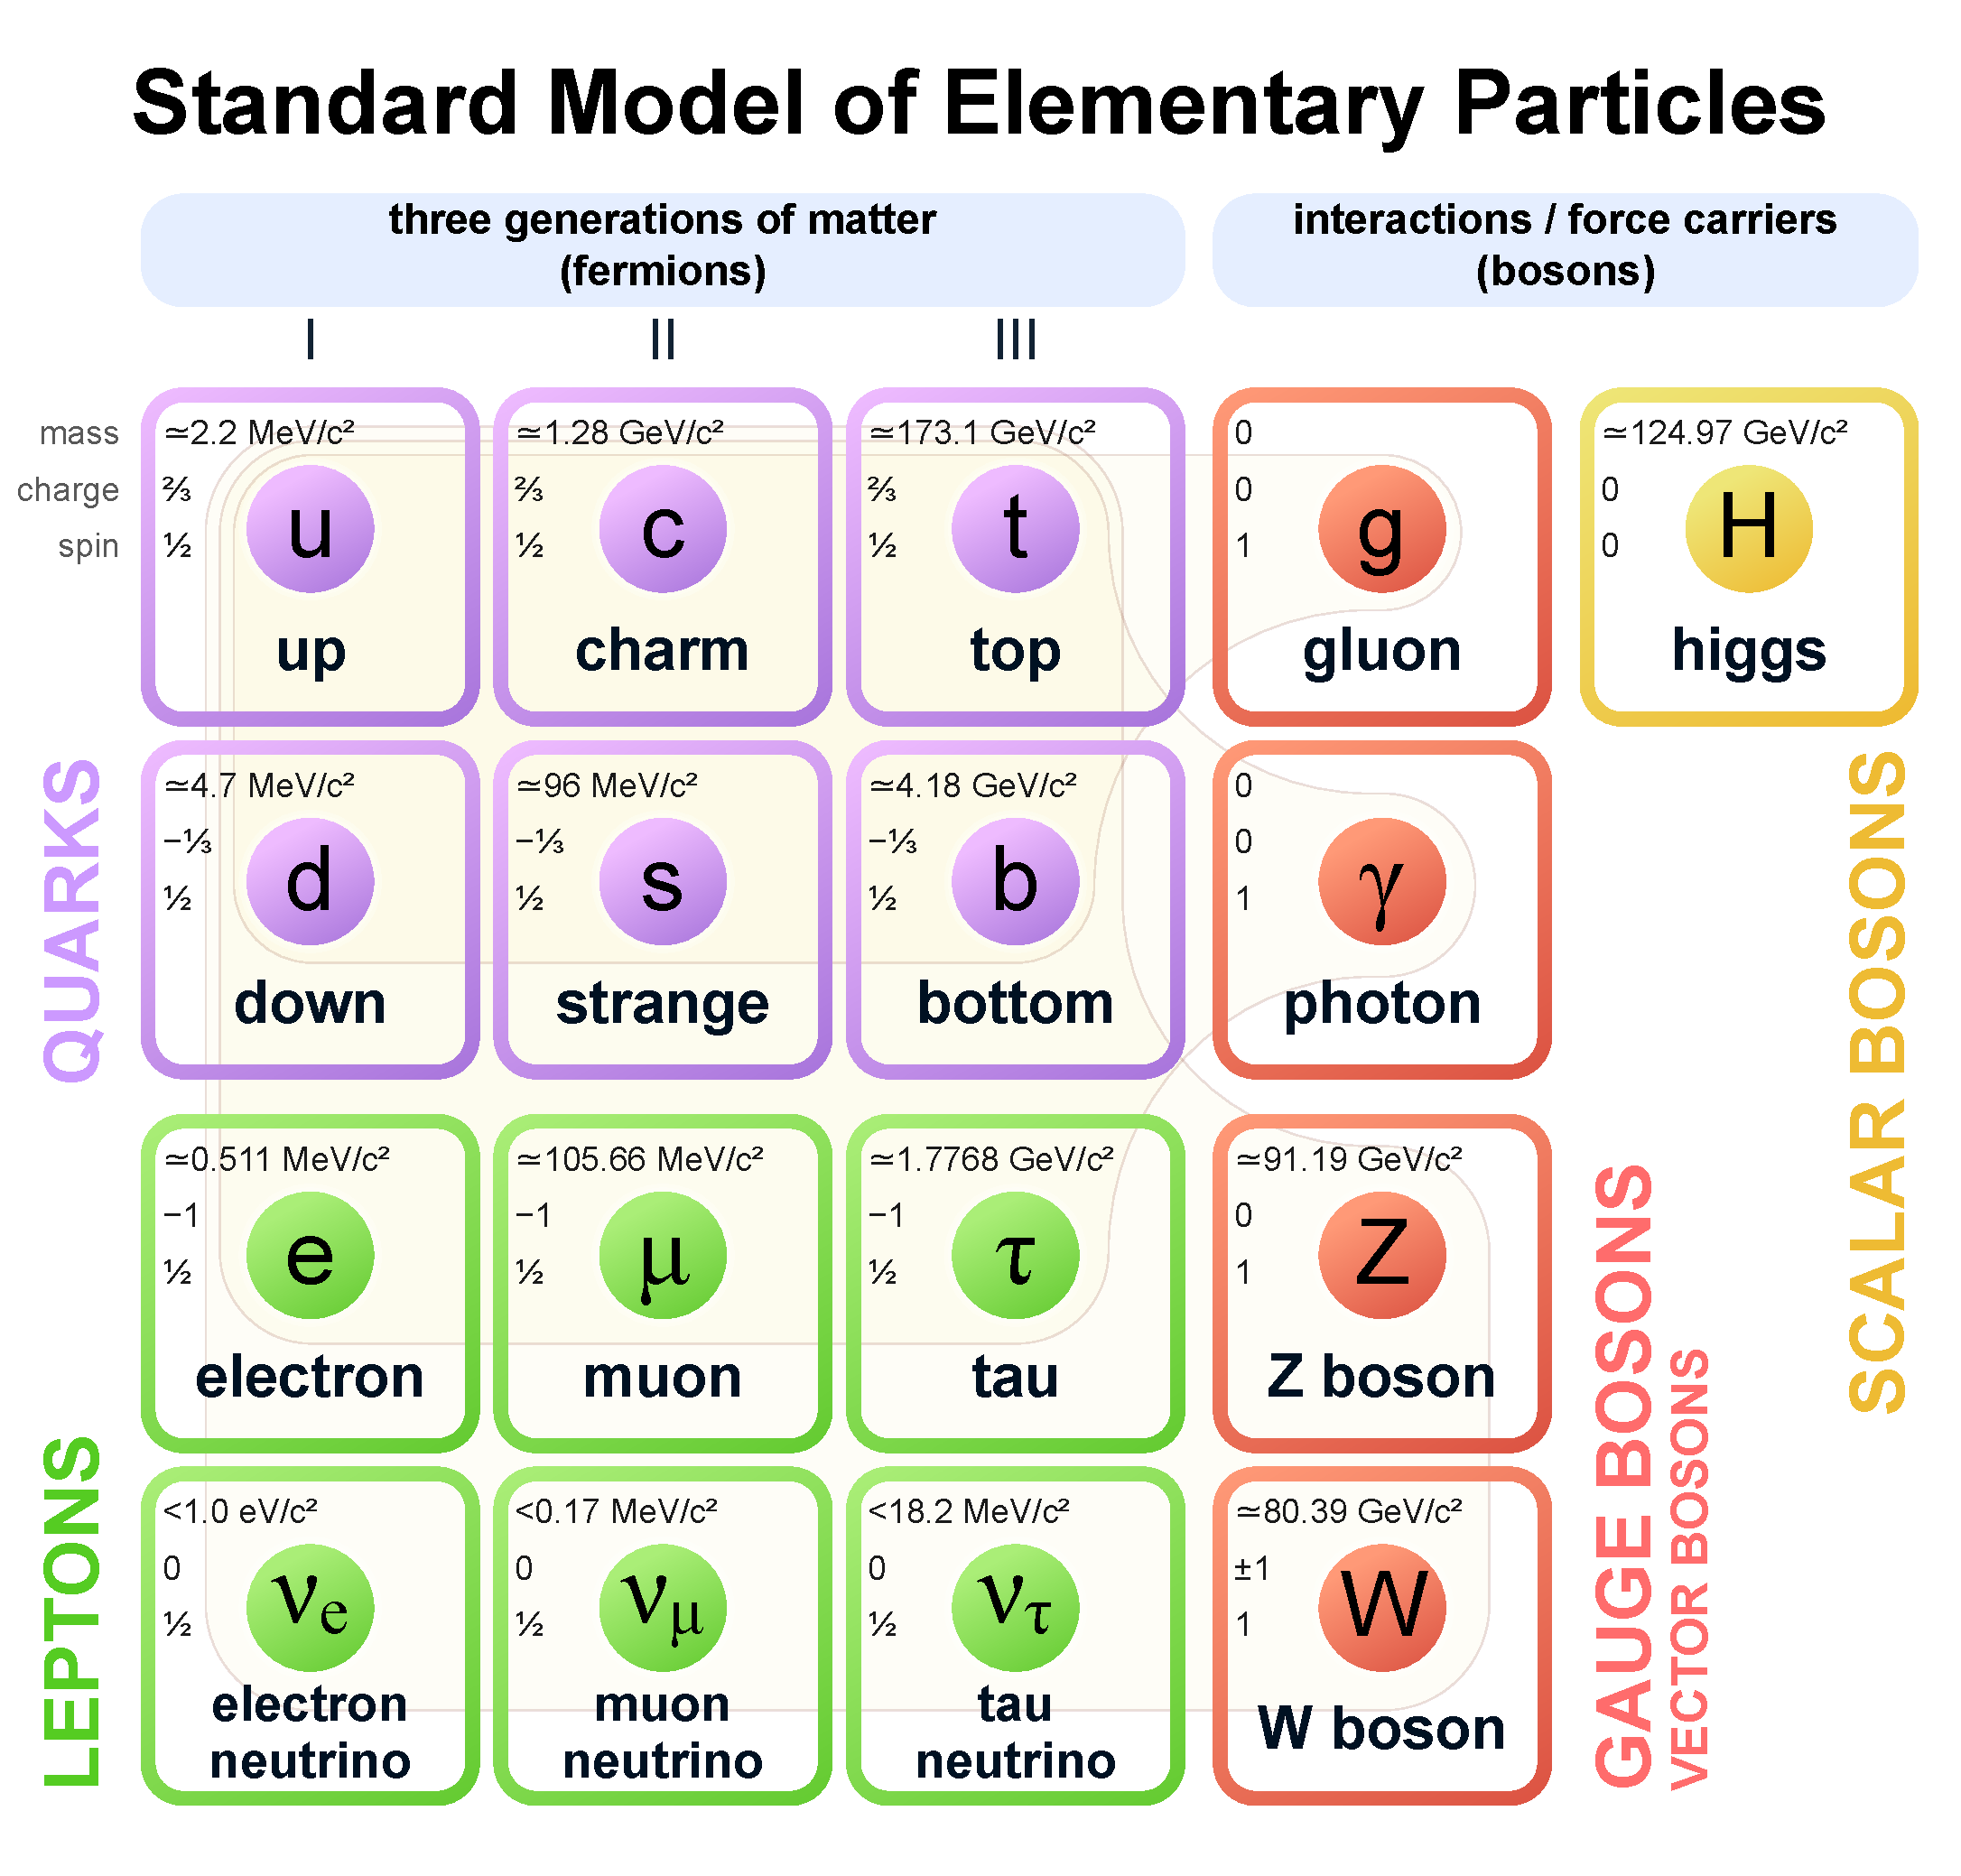
\includegraphics[width=0.9\textwidth]{fig/standard_model.pdf}
    \caption{
        The Standard Model.
    }
    \label{fig:standard_model}
\end{figure}

\subsection{Feynman diagrams}
Fortunately, there is way to encode essential Standard Model calculations in a simple drawing, so-called ``Feynman diagrams,'' which, consequently, help experimentalists keep track of physically allowed processes. 
In these pictures, time flows from left to right, while space is abstractly represented on the vertical axis\footnotemark{}. 
\footnotetext{In some dark corners of the physics community, these axes are switched, but this dissertation will not deviate from the configuration described here.}
The fundamental particles are represented by lines, and the intersections of three or four of these lines (Fig.~\ref{fig:sm_vertices}) represent interactions between the corresponding particles, so at least one of them must be a boson. 
For example, an electron emitting a photon (Fig.~\ref{fig:qed1}) is represented by an electron coming in from the left, the turning into a photon and an electron leaving the picture to the right. 
This same vertex can be rotated clockwise, such that it instead depicts the annihilation of an electron and positron into a photon (Fig.~\ref{fig:ee_to_g})---one of the electrons had to be replaced with its anti-particle (a positron) to conserve charge. 
Rotating it again, we see that it now represents an electron absorbing a photon (Fig.~\ref{fig:eg_to_e}). 
These vertices act as building blocks that can be rotated and fit together according to a set of rules that correspond to real physical laws. 
Thus, any fundamental physical process (e.g. Fig.~\ref{fig:beta_decay}) can be represented with a Feynman diagram. 
Feynman diagrams are not only a visual aid for remembering which processes are allowed, however, for they also encode precise calculations about that process which can, importantly, be verified by experiment.

\begin{figure}[htb]
    \centering
    \subfloat[]{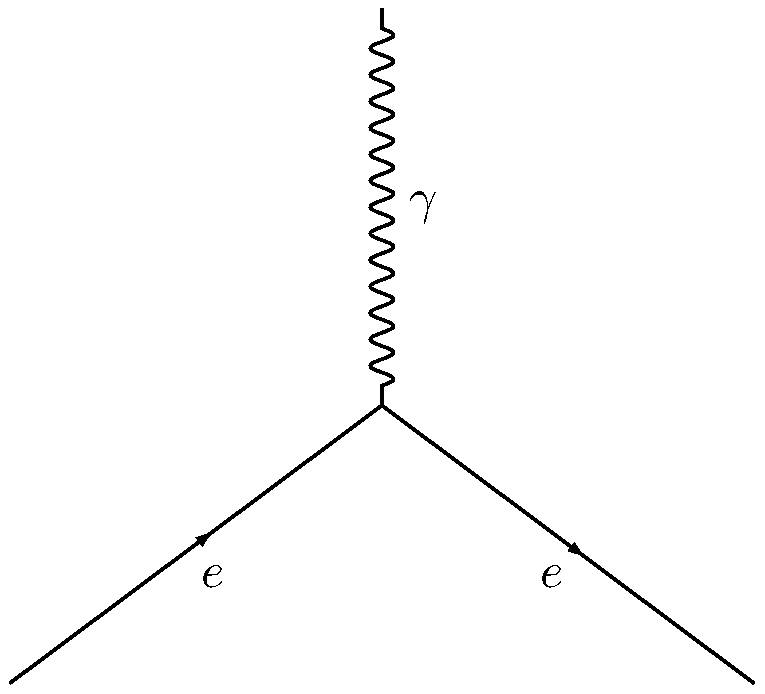
\includegraphics[width=0.25\textwidth]{fig/feynman/forces/qed_vertex.pdf}\label{fig:qed1}}\quad
    \subfloat[]{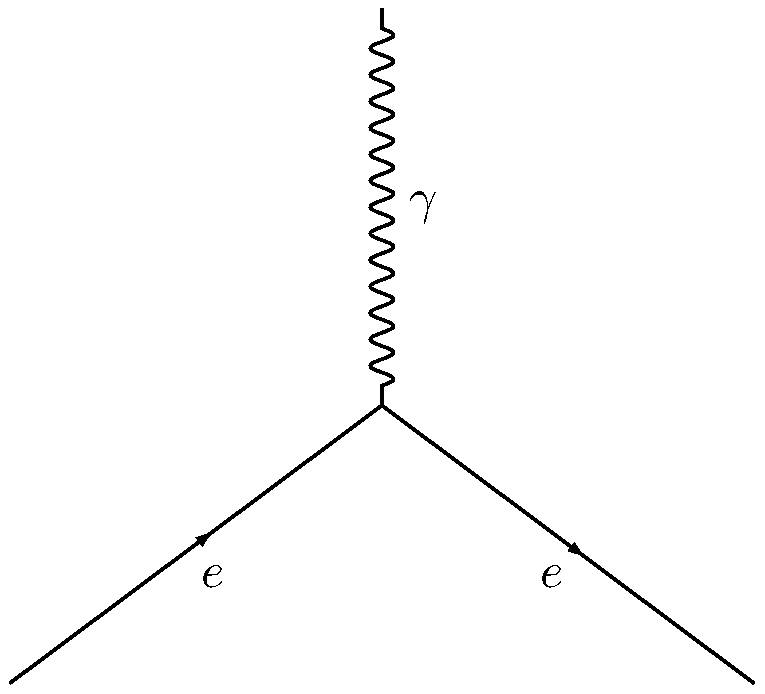
\includegraphics[width=0.25\textwidth]{fig/feynman/forces/qed_vertex.pdf}\label{fig:ewk1}}\quad
    \subfloat[]{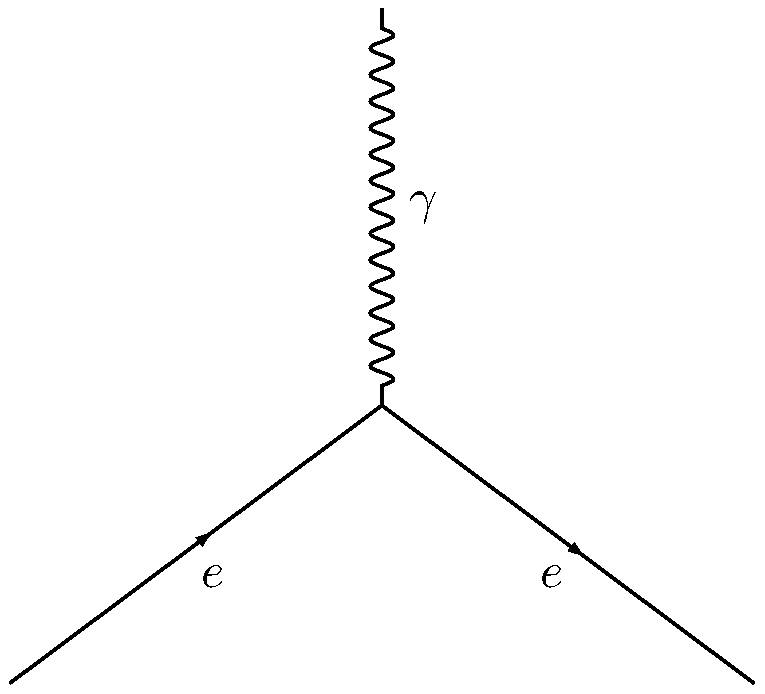
\includegraphics[width=0.25\textwidth]{fig/feynman/forces/qed_vertex.pdf}\label{fig:ewk2}}\\
    \subfloat[]{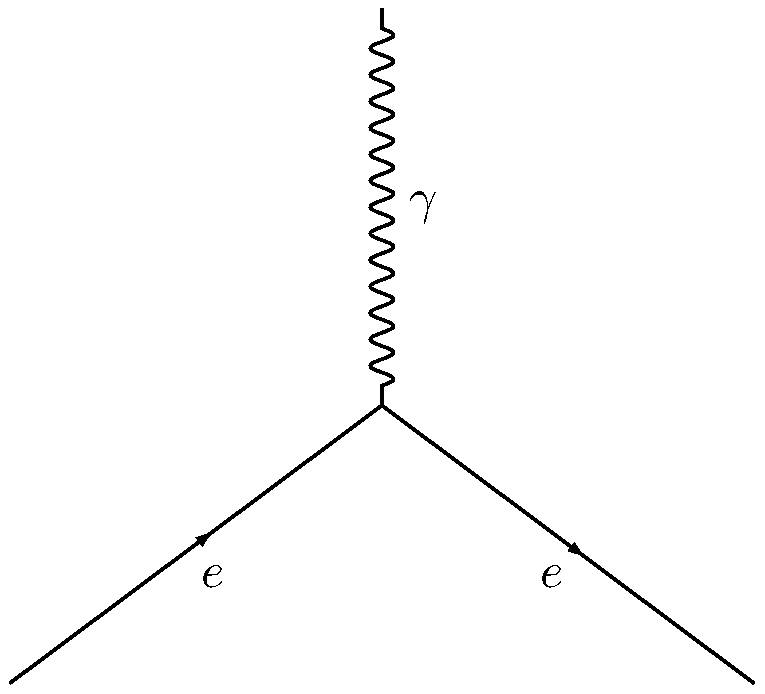
\includegraphics[width=0.25\textwidth]{fig/feynman/forces/qed_vertex.pdf}\label{fig:weak}}\quad
    \subfloat[]{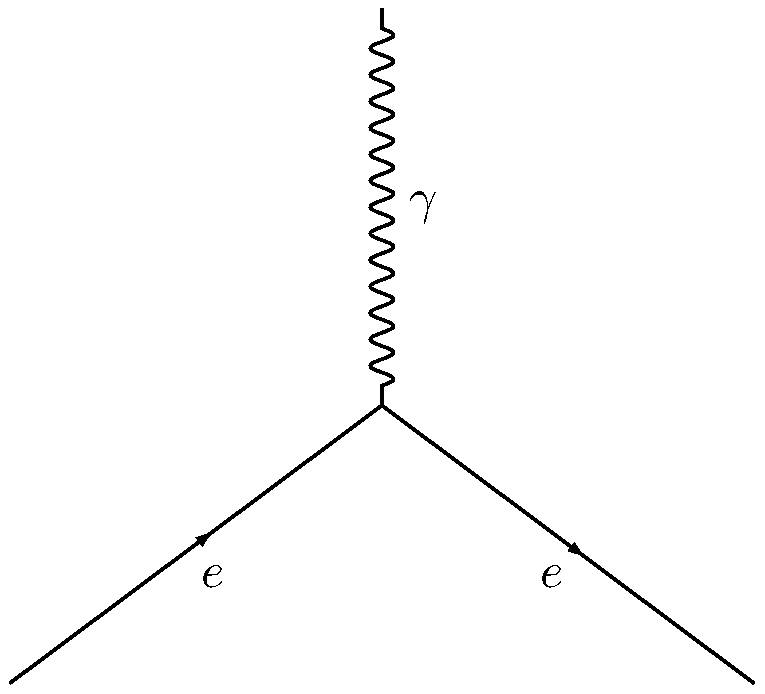
\includegraphics[width=0.25\textwidth]{fig/feynman/forces/qed_vertex.pdf}\label{fig:qcd1}}\quad
    \subfloat[]{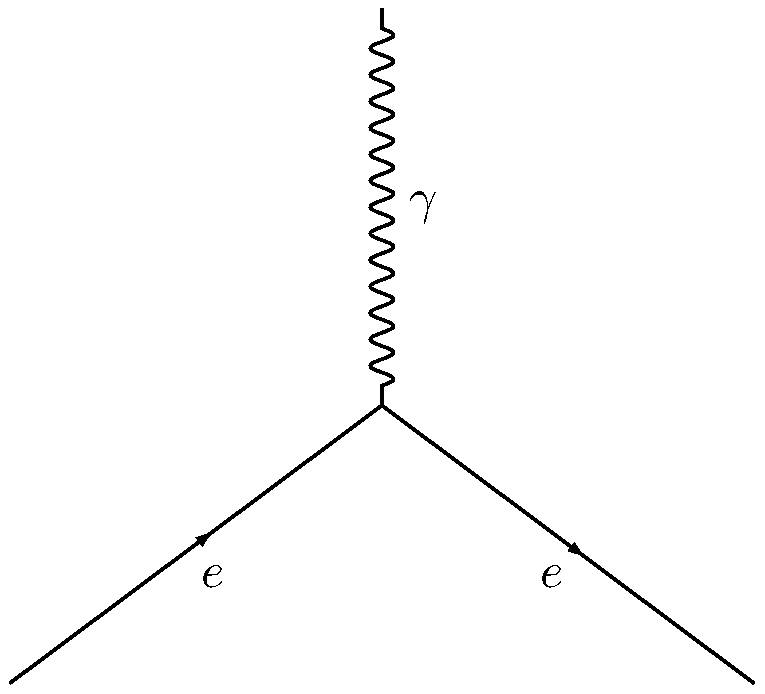
\includegraphics[width=0.25\textwidth]{fig/feynman/forces/qed_vertex.pdf}\label{fig:qcd2}}\\
    \subfloat[]{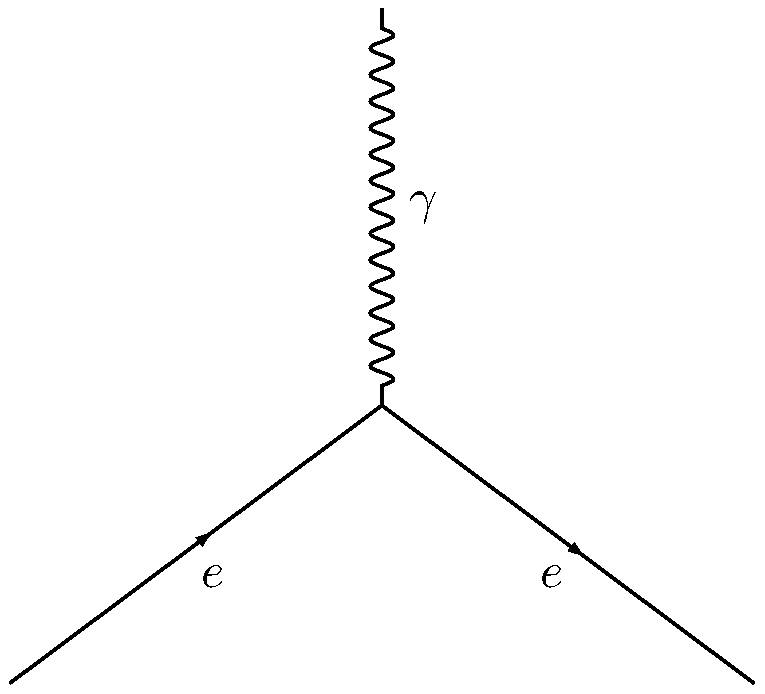
\includegraphics[width=0.25\textwidth]{fig/feynman/forces/qed_vertex.pdf}\label{fig:qcd3}}\quad
    \subfloat[]{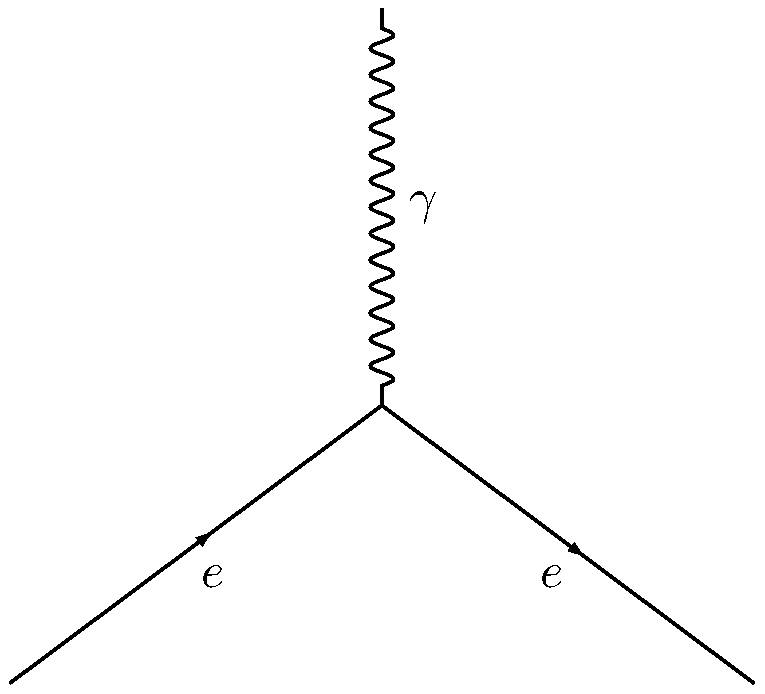
\includegraphics[width=0.25\textwidth]{fig/feynman/forces/qed_vertex.pdf}\label{fig:hig1}}\quad
    \subfloat[]{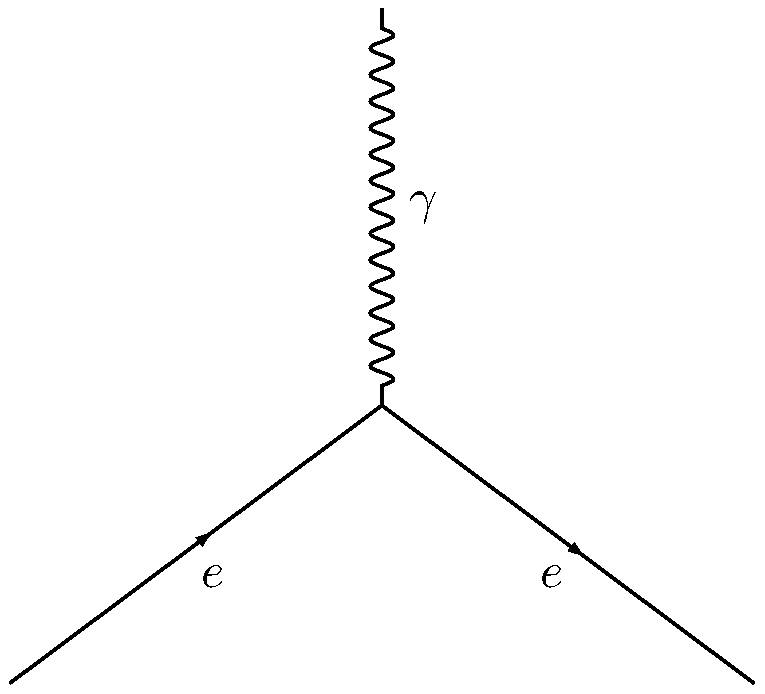
\includegraphics[width=0.25\textwidth]{fig/feynman/forces/qed_vertex.pdf}\label{fig:hig2}}
    \caption{
        The fundamental vertices in the Standard Model. 
        From left to right, top to bottom: 
        (a) electromagnetic; (b), (c) electroweak; (d) weak; (e), (f), (g) strong; (h), (i) Higgs. 
    }
    \label{fig:sm_vertices}
\end{figure}

\begin{figure}[htb]
    \centering
    \subfloat[$\Pem\to\PGg+\Pem$]{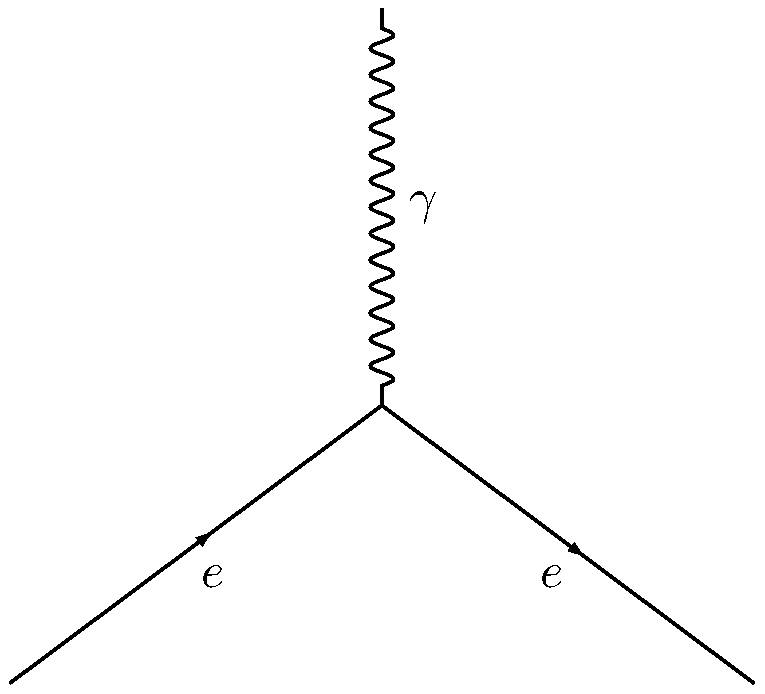
\includegraphics[width=0.25\textwidth]{fig/feynman/forces/qed_vertex.pdf}\label{fig:e_to_ge}}\quad
    \subfloat[$\Pep+\Pem\to\PGg$]{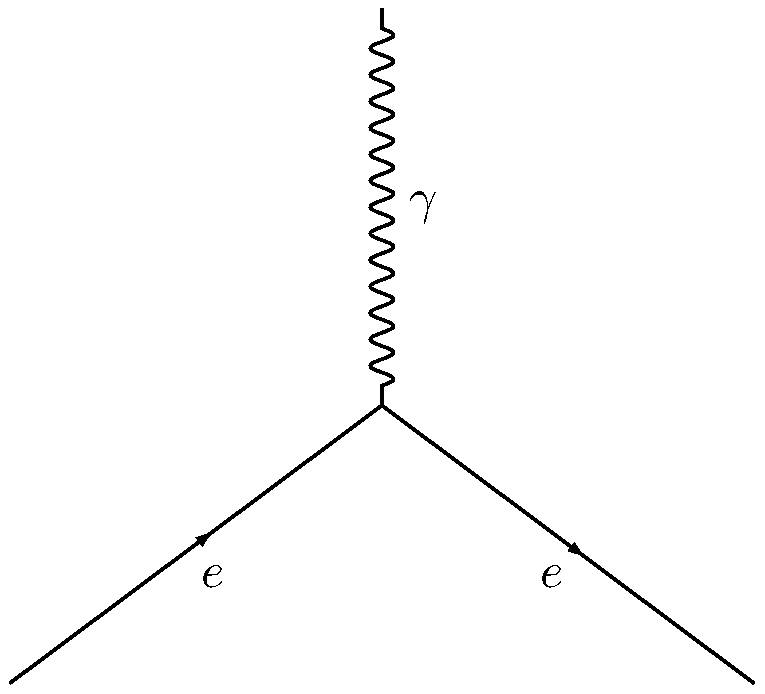
\includegraphics[width=0.25\textwidth]{fig/feynman/forces/qed_vertex.pdf}\label{fig:ee_to_g}}\quad
    \subfloat[$\Pem+\PGg\to\Pem$]{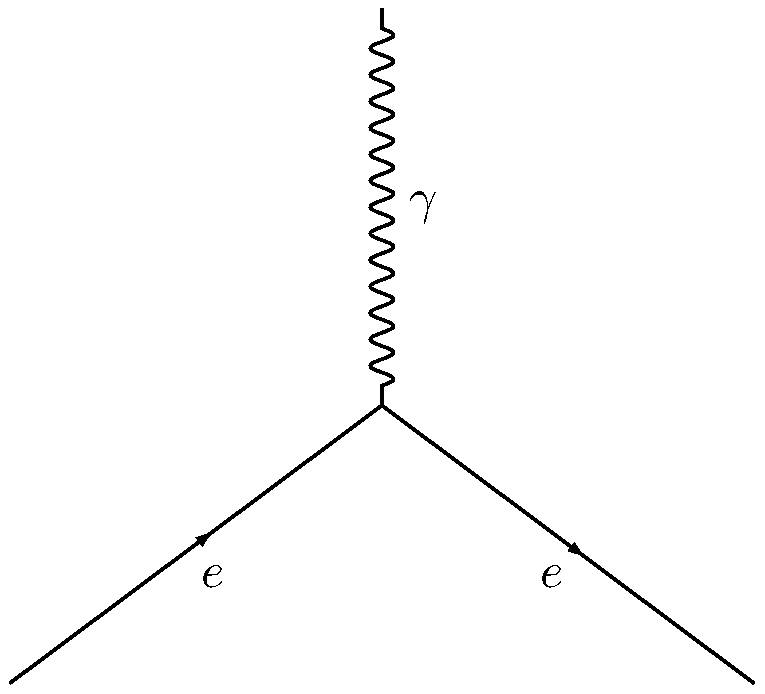
\includegraphics[width=0.25\textwidth]{fig/feynman/forces/qed_vertex.pdf}\label{fig:eg_to_e}}
    \caption{
        Rotations of the QED vertex, showing (a) an electron emitting a photon, (b) an electron and positron annihilating and producing a photon, and (c) an electron absorbing a photon. 
    }
    \label{fig:qed_rotations}
\end{figure}

\begin{figure}[htb]
    \centering
    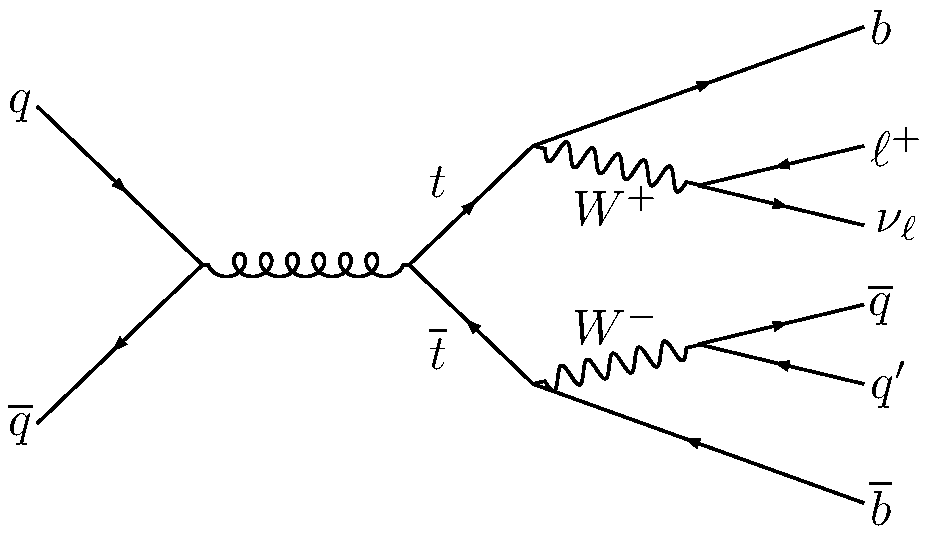
\includegraphics[width=0.6\textwidth]{fig/feynman/ttbar/ttbar_onelep.pdf} % FIXME: missing!!
    \caption{
        Feynman diagram for beta decay, which is mechanism behind the radioactive decay of certain elements. 
    }
    \label{fig:beta_decay}
\end{figure}

\subsection{Cross sections}
Consider two electrons barrelling towards each other with some velocity. 
In the classical picture, the electrons glance off one another and fly off to infinity at some angle to their original trajectories---like two errant ice skaters. 
This can be represented as a Feynman diagram (Fig.~\ref{fig:ee_scattering}) which is assembled from two EM vertices. 
Again, time flows from left to right, showing the two electrons entering, then the exchange of a photon, followed by the two electrons leaving, much like the classical picture. 
Now, suppose we construct two beams of electrons, aim them at each other, then turn them on (preferably after we leave the room). 
In this scenario, we may well want to know the probability that the two electrons will bounce off hach other (``scatter''). 
This probability is called the ``cross section,'' because it is mathematically similar to the classical picture\footnotemark{}, where we would compute the cross-sectional area presented to either of the colliding objects. 
\footnotetext{
    In fact, the answer to this question is expressed in the units of ``barns,'' literally as in ``hitting the broad side of a barn,'' coined by during World War II. % citatin needed
}
Indeed, one of the most important features of QFT is the ability to compute the cross section for scattering two electrons off of each other, as in this case, or any other interactions between particles. 
Feynman diagrams beautifully encode the complex mathematics at work here: each line and every vertex (where three lines meet) correspond a term in the calculation. 
While, again, the mathematical details are beyond the scope of this document, it is important to realize that the Feynman diagram can be directly used to calculate the cross section ($\sigma$):
\begin{equation}
    \sigma = \langle|\mathcal{M}|^2\rangle = \frac{2g_e^4}{(p_1 \cdot p_3)^2(p_1 \cdot p_4)^2[(p_1 \cdot p_2)^4 + (p_1 \cdot p_3)^4 + (p_1 \cdot p_4)^4]}
\end{equation}
where $p_1$ and $p_2$ are the four-momenta of the incoming electrons, $p_3, p_4$ are the four-momenta of the outgoing electrons, and $g_e$ is the EM coupling constant. 
This exercise, and the compact answer above, serves to demonstrate the sheer complexity of QFT calculations. 
Many details were left out beyond the computation itself (which is already a glaring omission), including details surrounding the spin of the electron, the definition of spin, the defition of four-momentum (and special relativity), and so on. 
Those details, and much more, can be found in the illustrious textbook from which this entire example was borrowed~\cite{Griffiths}. 
Moreover, this feature of QFT---the ability to compute cross sections---is absolutely vital because it offers a way of testing the theory with observation: compute the probability that the event is expected to occur, then try to reproduce that event many times in the lab and see how many times it really happens. 

\begin{figure}[htb]
    \centering
    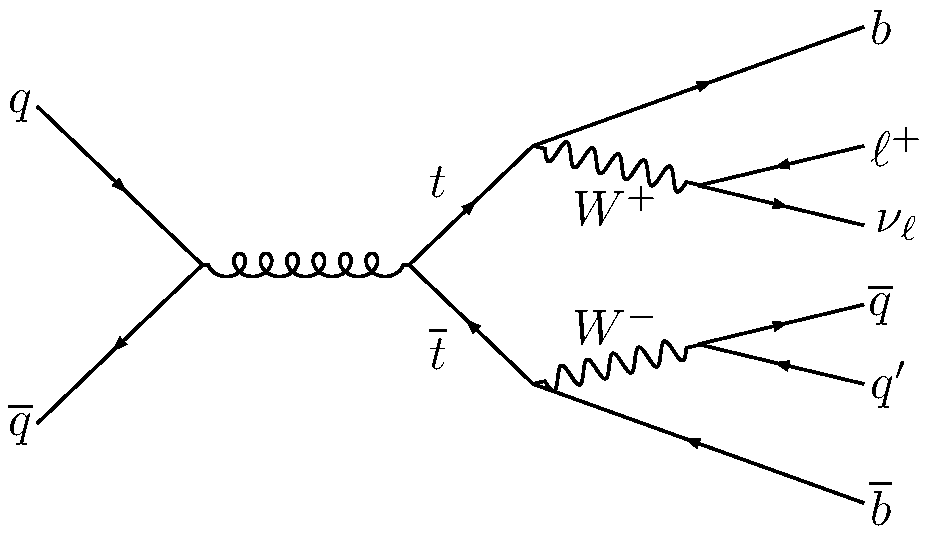
\includegraphics[width=0.6\textwidth]{fig/feynman/ttbar/ttbar_onelep.pdf} % FIXME: missing!!
    \caption{
        Feynman diagram for electron-electron scattering. 
    }
    \label{fig:ee_scattering}
\end{figure}

The validity of any model is a precarious condition: the model must exactly describe reality, else it is not a realization of the truth, but rather only approximately---or worse, accidentally---correct. 
That is, \textit{every} SM cross section value must be accurate for the validity of the model to hold. 
And so generations of physicists have made dilligent, and highly accurate, measurements of a dozens of cross sections---spanning orders of magnitude of rarity. 
Tabulated in grand tables (Fig.~\ref{fig:cms_xsecs} and \ref{fig:atlas_xsecs}), it is evident that the Standard Model has so far withstood every test derived from CMS data and ATLAS data. 
This is an incredible feat: a ``simple'' model seems to describe subatomic physics, which drove the creation of the universe and continues to drive the mechanics of everything, with incredible accuracy. 
Lingering beyond these shining trophies, however, are a number of glaring inconsistencies and enormous missing pieces. 
In other words, we know with certainty that the Standard Model is not complete, and that much more work is needed to complete it. 
We will focus in this dissertation on questions around the Higgs boson, these are detailed in the next section, because these questions motivated the bulk of the work described in the following chapters. 
However, we will also mention some additional open questions to illustrate the magnitude of the problem ahead for future particle physicists. 

\begin{figure}[htb]
    \centering
    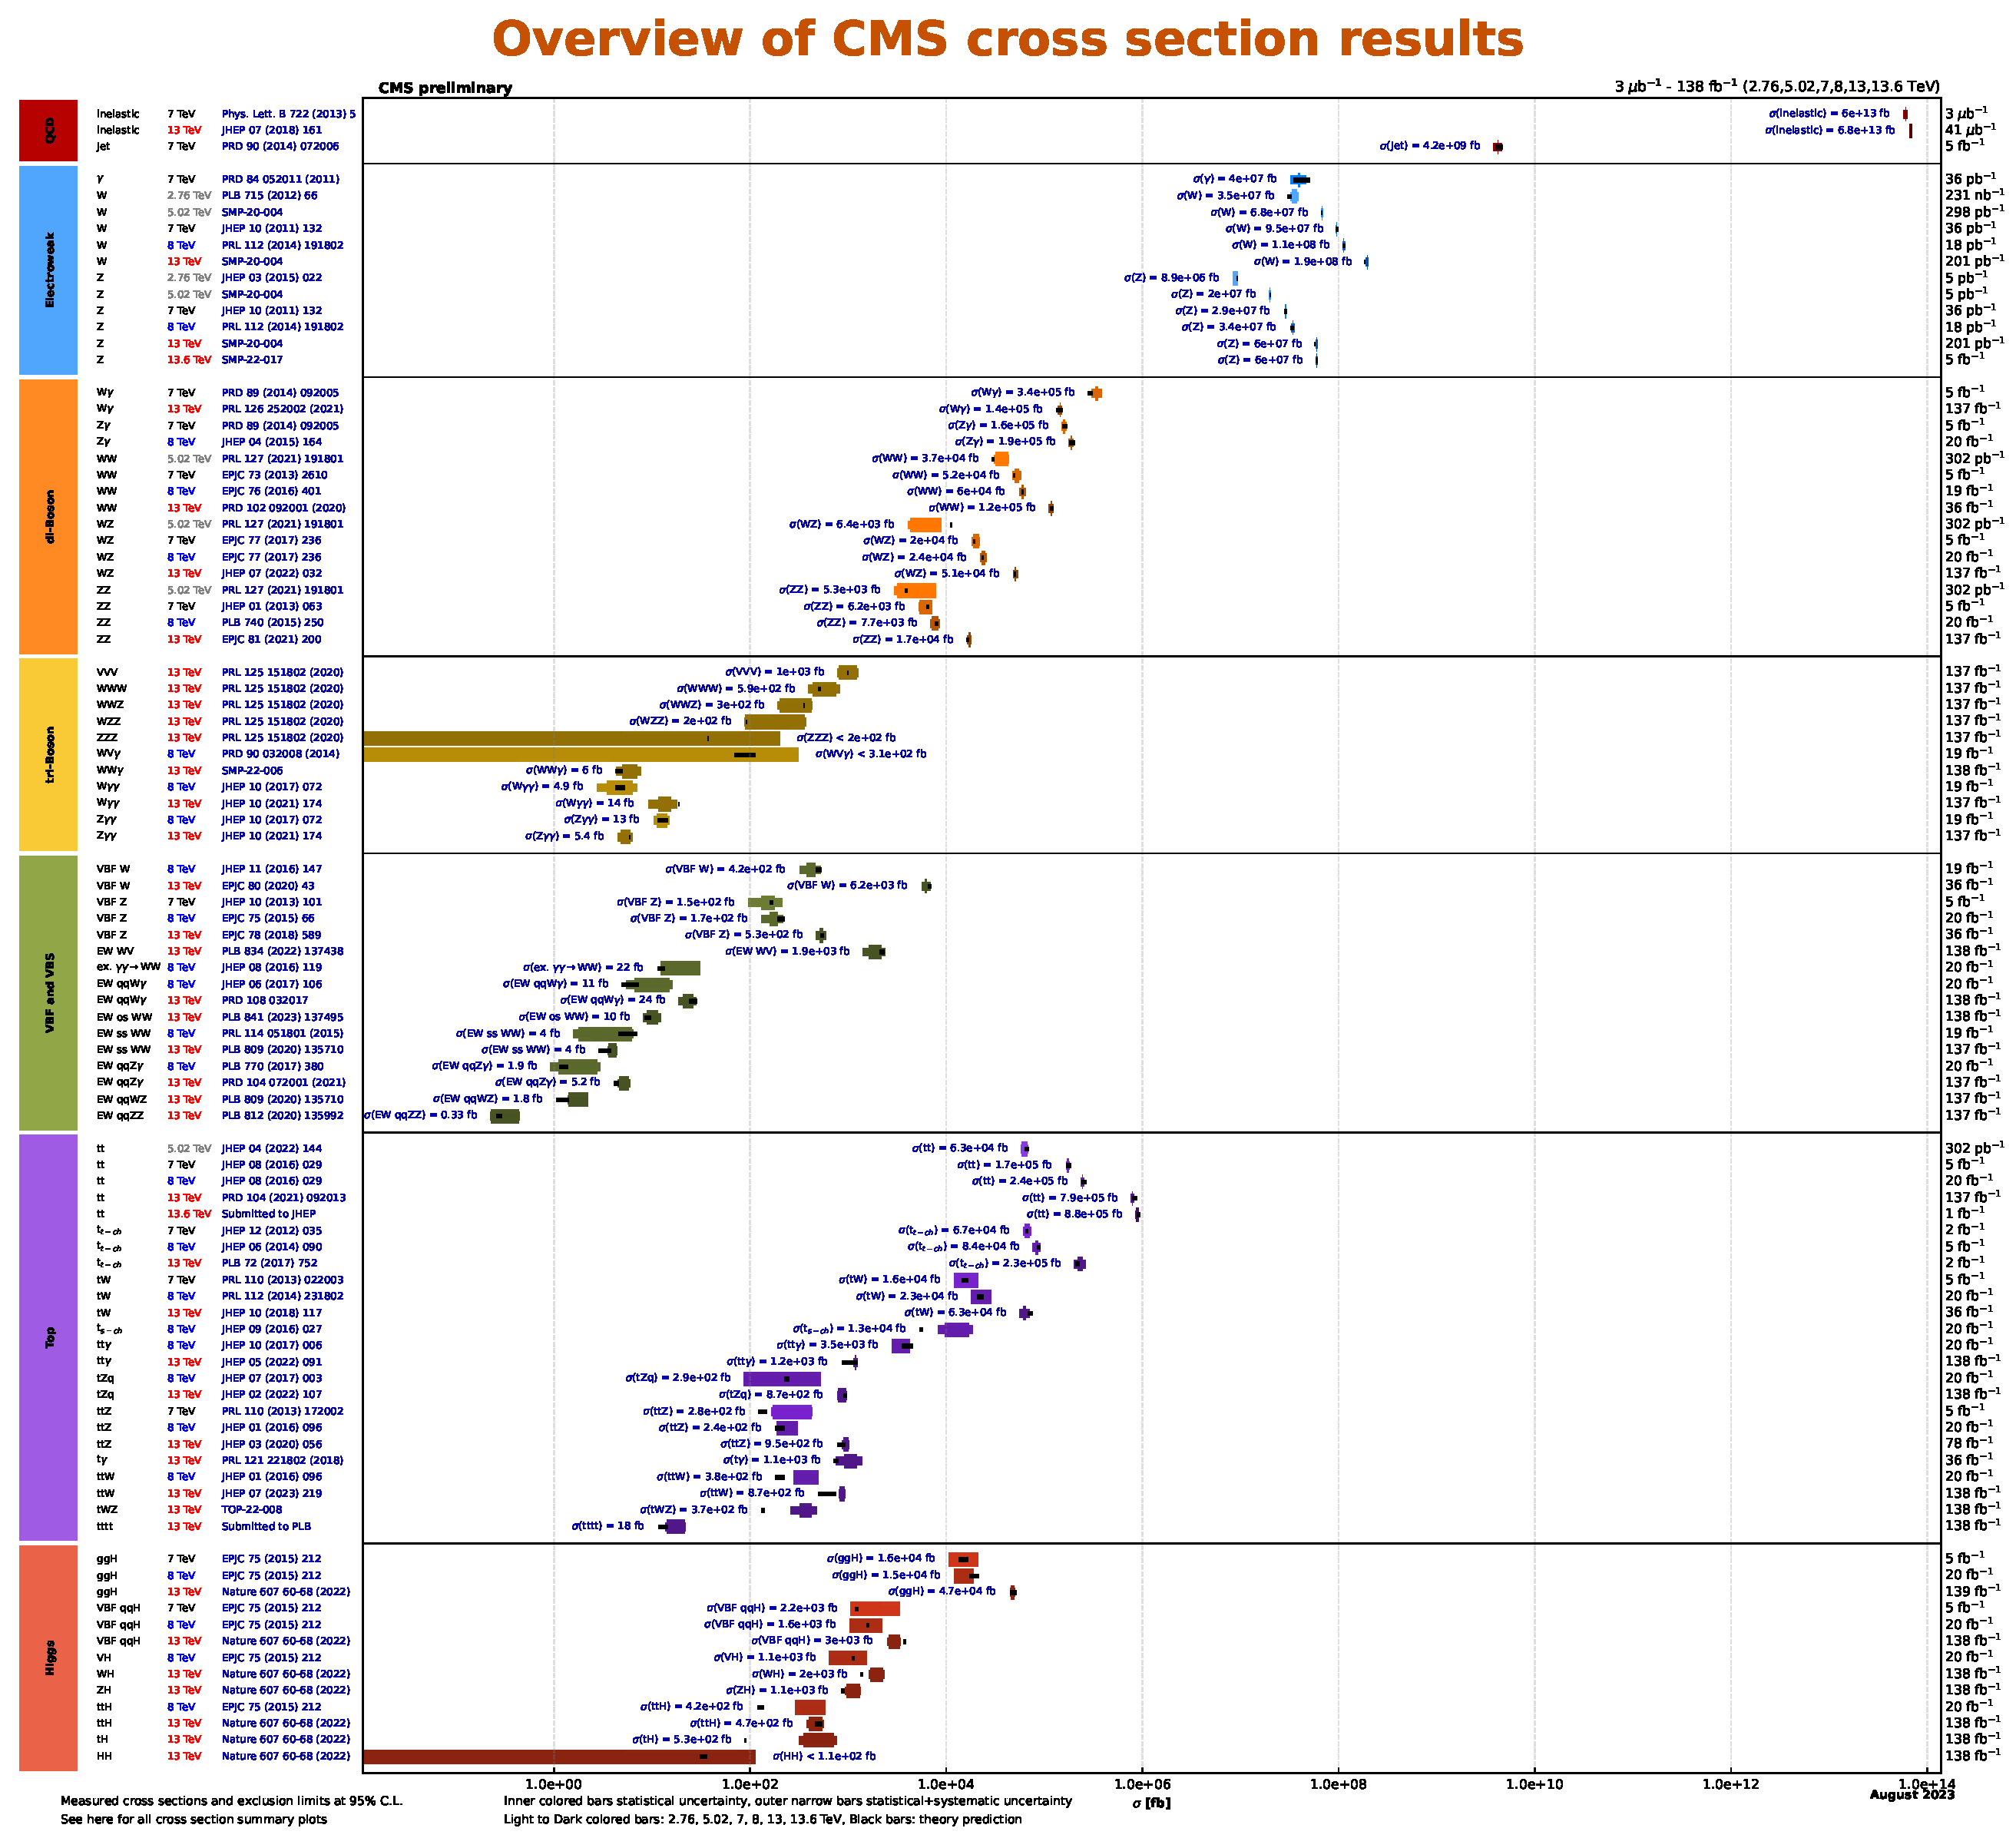
\includegraphics[width=0.9\textwidth]{fig/cms/cms_xsecs_2023.pdf}
    \caption{
        The totality of the cross section measurements performed with data from the CMS Experiment compared to the Standard Model predictions. 
        Precise agreement with the Standard Model can be seen across several orders of magnitude, representing the triumph of the model across decades of experimental scrutiny. 
        Plot taken from Ref.~\cite{CMSXSecs}.
    }
    \label{fig:cms_xsecs}
\end{figure}

\begin{figure}[htb]
    \centering
    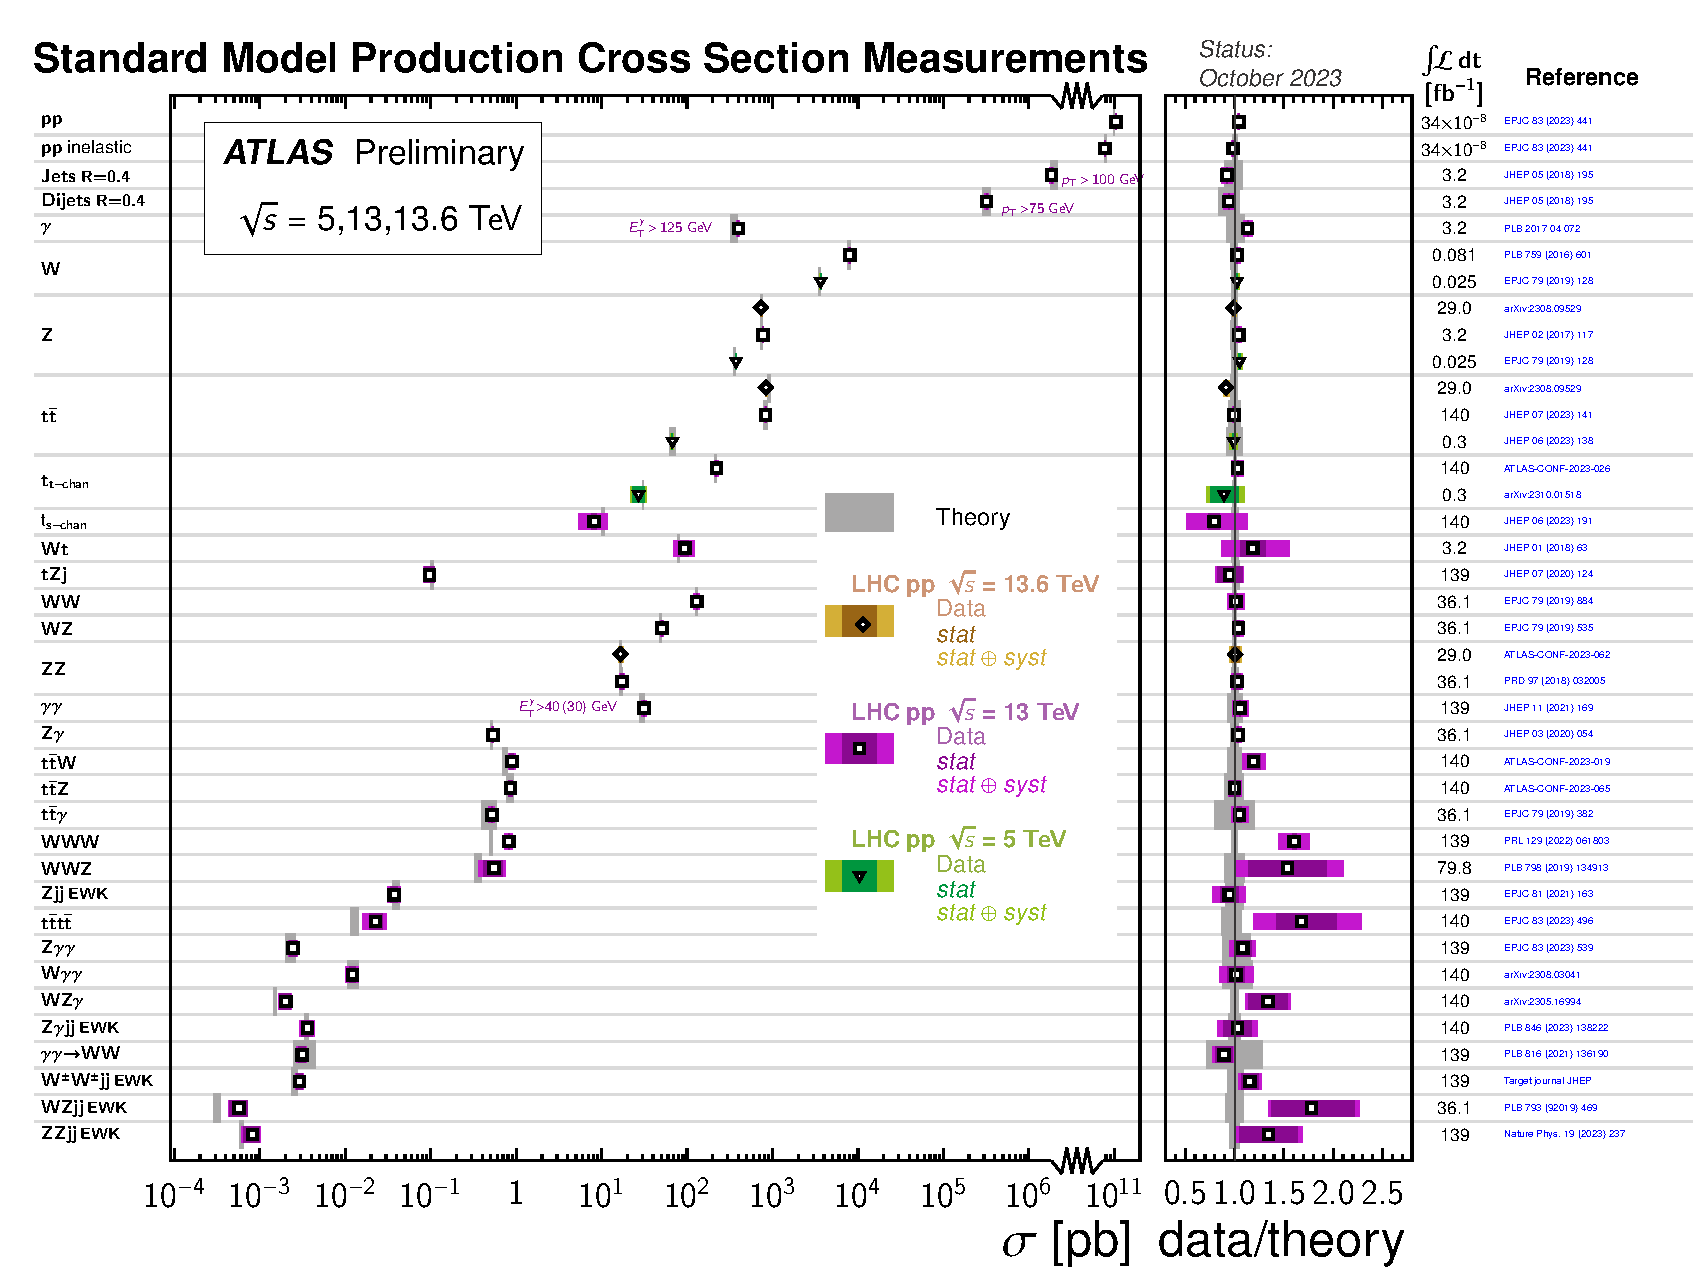
\includegraphics[width=0.9\textwidth]{fig/atlas/atlas_xsecs_2023.pdf}
    \caption{
        A selection of cross section measurements performed with data from the ATLAS Experiment compared to the Standard Model predictions. 
        Precise agreement with the Standard Model can be seen across several orders of magnitude, representing the triumph of the model across decades of experimental scrutiny. 
        Plot taken from Ref.~\cite{ATL-PHYS-PUB-2023-039}.
    }
    \label{fig:atlas_xsecs}
\end{figure}

\subsection{The Higgs boson}
Because we swore to steer away from the details of QFT, we cannot define the Higgs boson and Higgs mechanism completely. 
For this, we are better served by a primer by Griffiths~\cite{Griffiths}, followed by the standard QFT textbooks, and finally the original papers on the subject~\cite{EnglertBroutPRL, HiggsPhysLett, HiggsPRL, GuralnikHagenKibblePRL}. % TODO: add citation for Schroeder, Schredniki, and maybe Schwartz?
Without these prerequisites, it suffices to say that the idea of the Higgs boson is deeply based in Lagrangian mechanics. 
Originally derived for classical systems---an arrow in flight, a planet in motion, a ball on a ramp---an appropriately written ``Lagrangian,'' a mathematical object, together with the Euler-Lagrange equation can reproduce the mathematical description of the dynamics of a given system---the position of the arrow, planets, or ball as a function of time. 
The Lagrangian $L$ is a simple function of the energies in a classical mechanics:
\begin{equation}
    L = \underbrace{\frac{1}{2}m\dot{x}^2}_\text{kinetic energy} - \underbrace{U(x)}_{\substack{\text{potential} \\ \text{energy}}}
\end{equation}
where $x$, really $x(t)$, is the position of some physical object in one direction as a function of time and $\dot{x}$ is shorthand for the derivative of x with respect to time ($\frac{d}{dt}$), or the velocity. 
By plugging $L$ into the Euler-Lagrange equations, we will be able to solve for $x(t)$ with some algebra and calculus: 
\begin{equation}
    \frac{d}{dt}\bigg(\frac{\partial L}{\partial\dot{x}}\bigg) = \frac{\partial L}{\partial x}
\end{equation}

In particle physics, we promote $x(t)$ to a field\footnotemark{} $\phi$, which is a function of space and time $\phi(x, y, z, t)$, and $L$ to $\mathcal{L}$, a Lagrangian \textit{density}.
\footnotetext{Fields are used here in a quantum context, scalar fields in particular, but there are many classical examples: the temperature of a room, the height of the sea, the strength of a magnetic field, these are quantities that may be different at every position in space and may also vary in time.}
Our interest in these abstract fields is well-motivated in QFT, where a field $\phi(x,y,z,t)$ with certain properties corresponds to an observable particle with those same properties. 
For example, the Lagrangian 
\begin{equation}
    \mathcal{L} = \underbrace{\frac{1}{2}(\partial_\mu\phi)(\partial^\mu\phi)}_{\text{kinetic term}} - \underbrace{\frac{1}{2}\big(\frac{mc}{\hbar}\big)^2}_\text{mass term}
\end{equation}
represents a spin-0 particle with mass $m$. 
As in classical machanics, plugging the appropriate Lagrangian density into the Euler-Lagrange equation yields the precise descriptions of the dynamics of fundamental particles. 

The Higgs mechanism arises when we try to write down a Lagrangian density $\mathcal{L}$ that accounts for the existence of the $\PW$ and $\PZ$ bosons. % for some reason, $$ are needed here, else the doc breaks
In doing so, we find that we must demand that $\mathcal{L}$ does not change under certain transformations of the fields $\phi$, which, at face value, equates to demanding that the field is massless---without going into details, this claim must simply be accepted as true. 
This is a problem because the $\PW$ and $\PZ$ bosons are verifiably not massless. % for some reason, $$ are needed here, else the doc breaks
However, by introducing two scalar fields---corresponding to the Higgs boson and Goldstone boson---and massaging the mathematics, a mass term emerges for the $\PW$ and $\PZ$ bosons. % for some reason, $$ are needed here, else the doc breaks
The Goldstone boson does not correspond to a real particle, but instead services the mathematics\footnotemark{} and disappears under a specific transformation. 
\footnotetext{For example, it accounts for the fact that there are three bosons that carry the weak force ($\PW^{+}$, $\PW^{-}$, $\PZ$).} % for some reason, $$ are needed here, else the doc breaks
The Higgs \textit{mechanism} itself refers to the appearance of the $\PW$ and $\PZ$ boson masses, as well as the fermion masses through different interactions~\cite{Weinberg:1967tq, Nambu:1961fr}. % for some reason, $$ are needed here, else the doc breaks

Beyond the blackboard, the Higgs mechanism gives us a picture of how the universe came to be: in the first moments of time, the fundamental particles were endowed with mass by the Higgs mechanism. 
Thus, rather than fly off to infinity at the speed of light, atoms were formed, and the universe as we know it bloomed.  
The Higgs boson is therefore essential to the origin and continued existence of the known universe---in fact, if the Higgs field were to spontaneously dissappear, the entire universe would evaporate in a nanosecond. % citation needed
It is also, however, a key to understanding the universe's distant future~\cite{Bass2021}: will the universe collapse or explode or something else entirely? % citation needed
We shall spare ourselves of existential crisis and instead simply appreciate the specific importance of the Higgs boson. 
While every piece of the Standard Model is important, just as every link in a chain, the Higgs boson is one of the less well-understood particles, and further study of this latest addition to the Standard Model may shed crucial light on the many open questions in particle physics. 

\section{Selected open questions}\label{sec:open_questions}
\subsection{What is dark matter?}
\subsection{What is dark energy?}
\subsection{Is the Higgs boson really a fundamental particle?}
\subsection{Is there only one Higgs boson?}
\subsection{Why is the Higgs boson mass so small?}
% Higgs sector:
%    - naturalness?
%    - other higgses?? Gell-Mann said something like "it would be weird if 
%      there was only one Higgs boson" in 2012 CERN interview
%    - other problems... I guess introduce problem of not yet measuring 
%      higgs couplings well
% More generic:
%    - dark matter

\chapter{A Grand Apparatus}\label{ch:lhc_cms}
\begin{aquote}{Fran\c{c}ois Englert, CMS: The Art of Science, 2016}
    A glance at the ATLAS and CMS detectors at CERN reveals their beauty...
    These detectors are the modern cathedrals of the rational world created by scientists, experimentalists, and theoreticians. 
\end{aquote}

\section{The Large Hadron Collider}
The Large Hadron Collider (LHC) is the largest particle accelerator ever built. 
Its most striking feature is a 27 km ring buried 100 m beneath the Franco-Swiss border (Fig.~\ref{fig:lhc_depth}) in which two beams of protons (or heavy ions like lead), after going through several smaller stages (Fig.~\ref{fig:cern_complex}), are accelerated to 99.9999991\% of the speed of light in opposite directions. 
The beams are steered by thousands of magnets, including 1232 superconducting dipole magnets (Fig.~\ref{fig:lhc_dipole}), placed along the circumference of the ring. 
At various points, the proton beams are directed towards each other, allowing the protons to collide. 
These collision points are surrounded by enormous, multi-layered particle detectors which record snapshots of the collisions. 

\begin{figure}[htb]
    \centering
    \subfloat{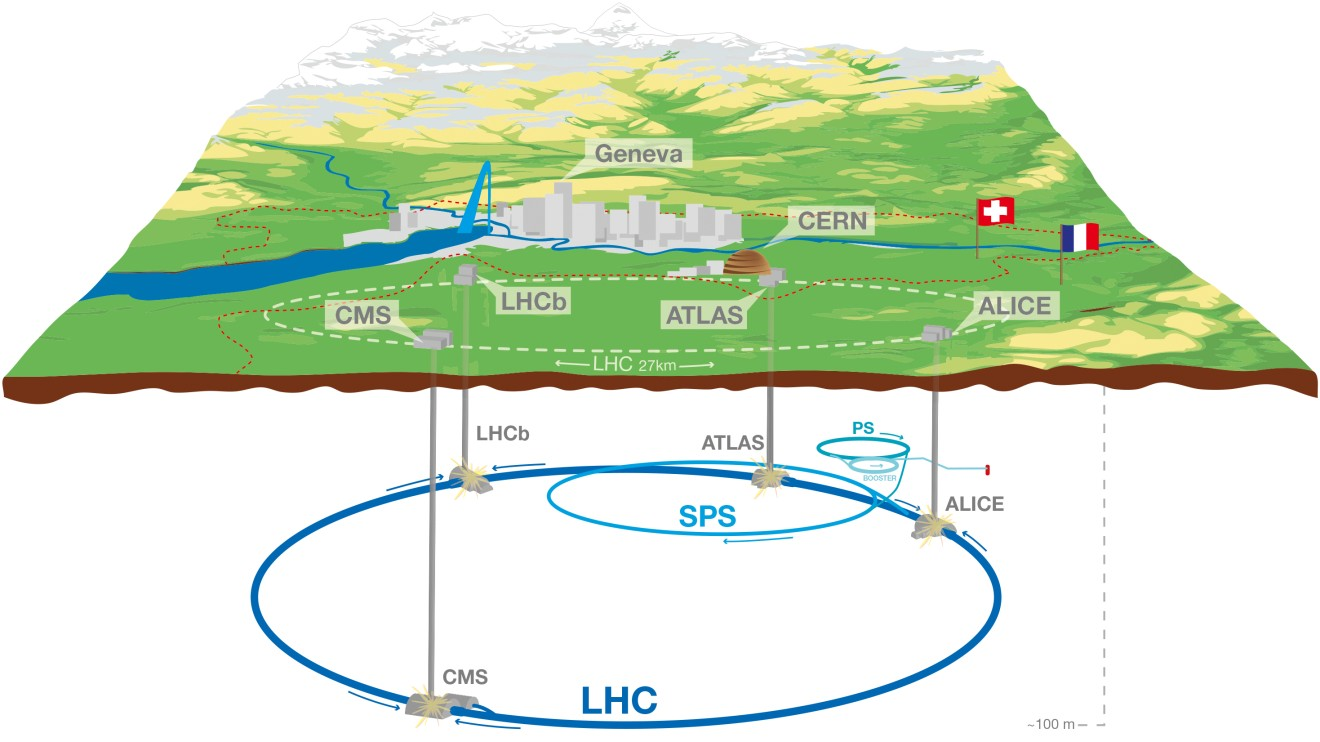
\includegraphics[width=0.45\textwidth,valign=c]{fig/lhc/lhc_depth.jpg}}\quad
    \subfloat{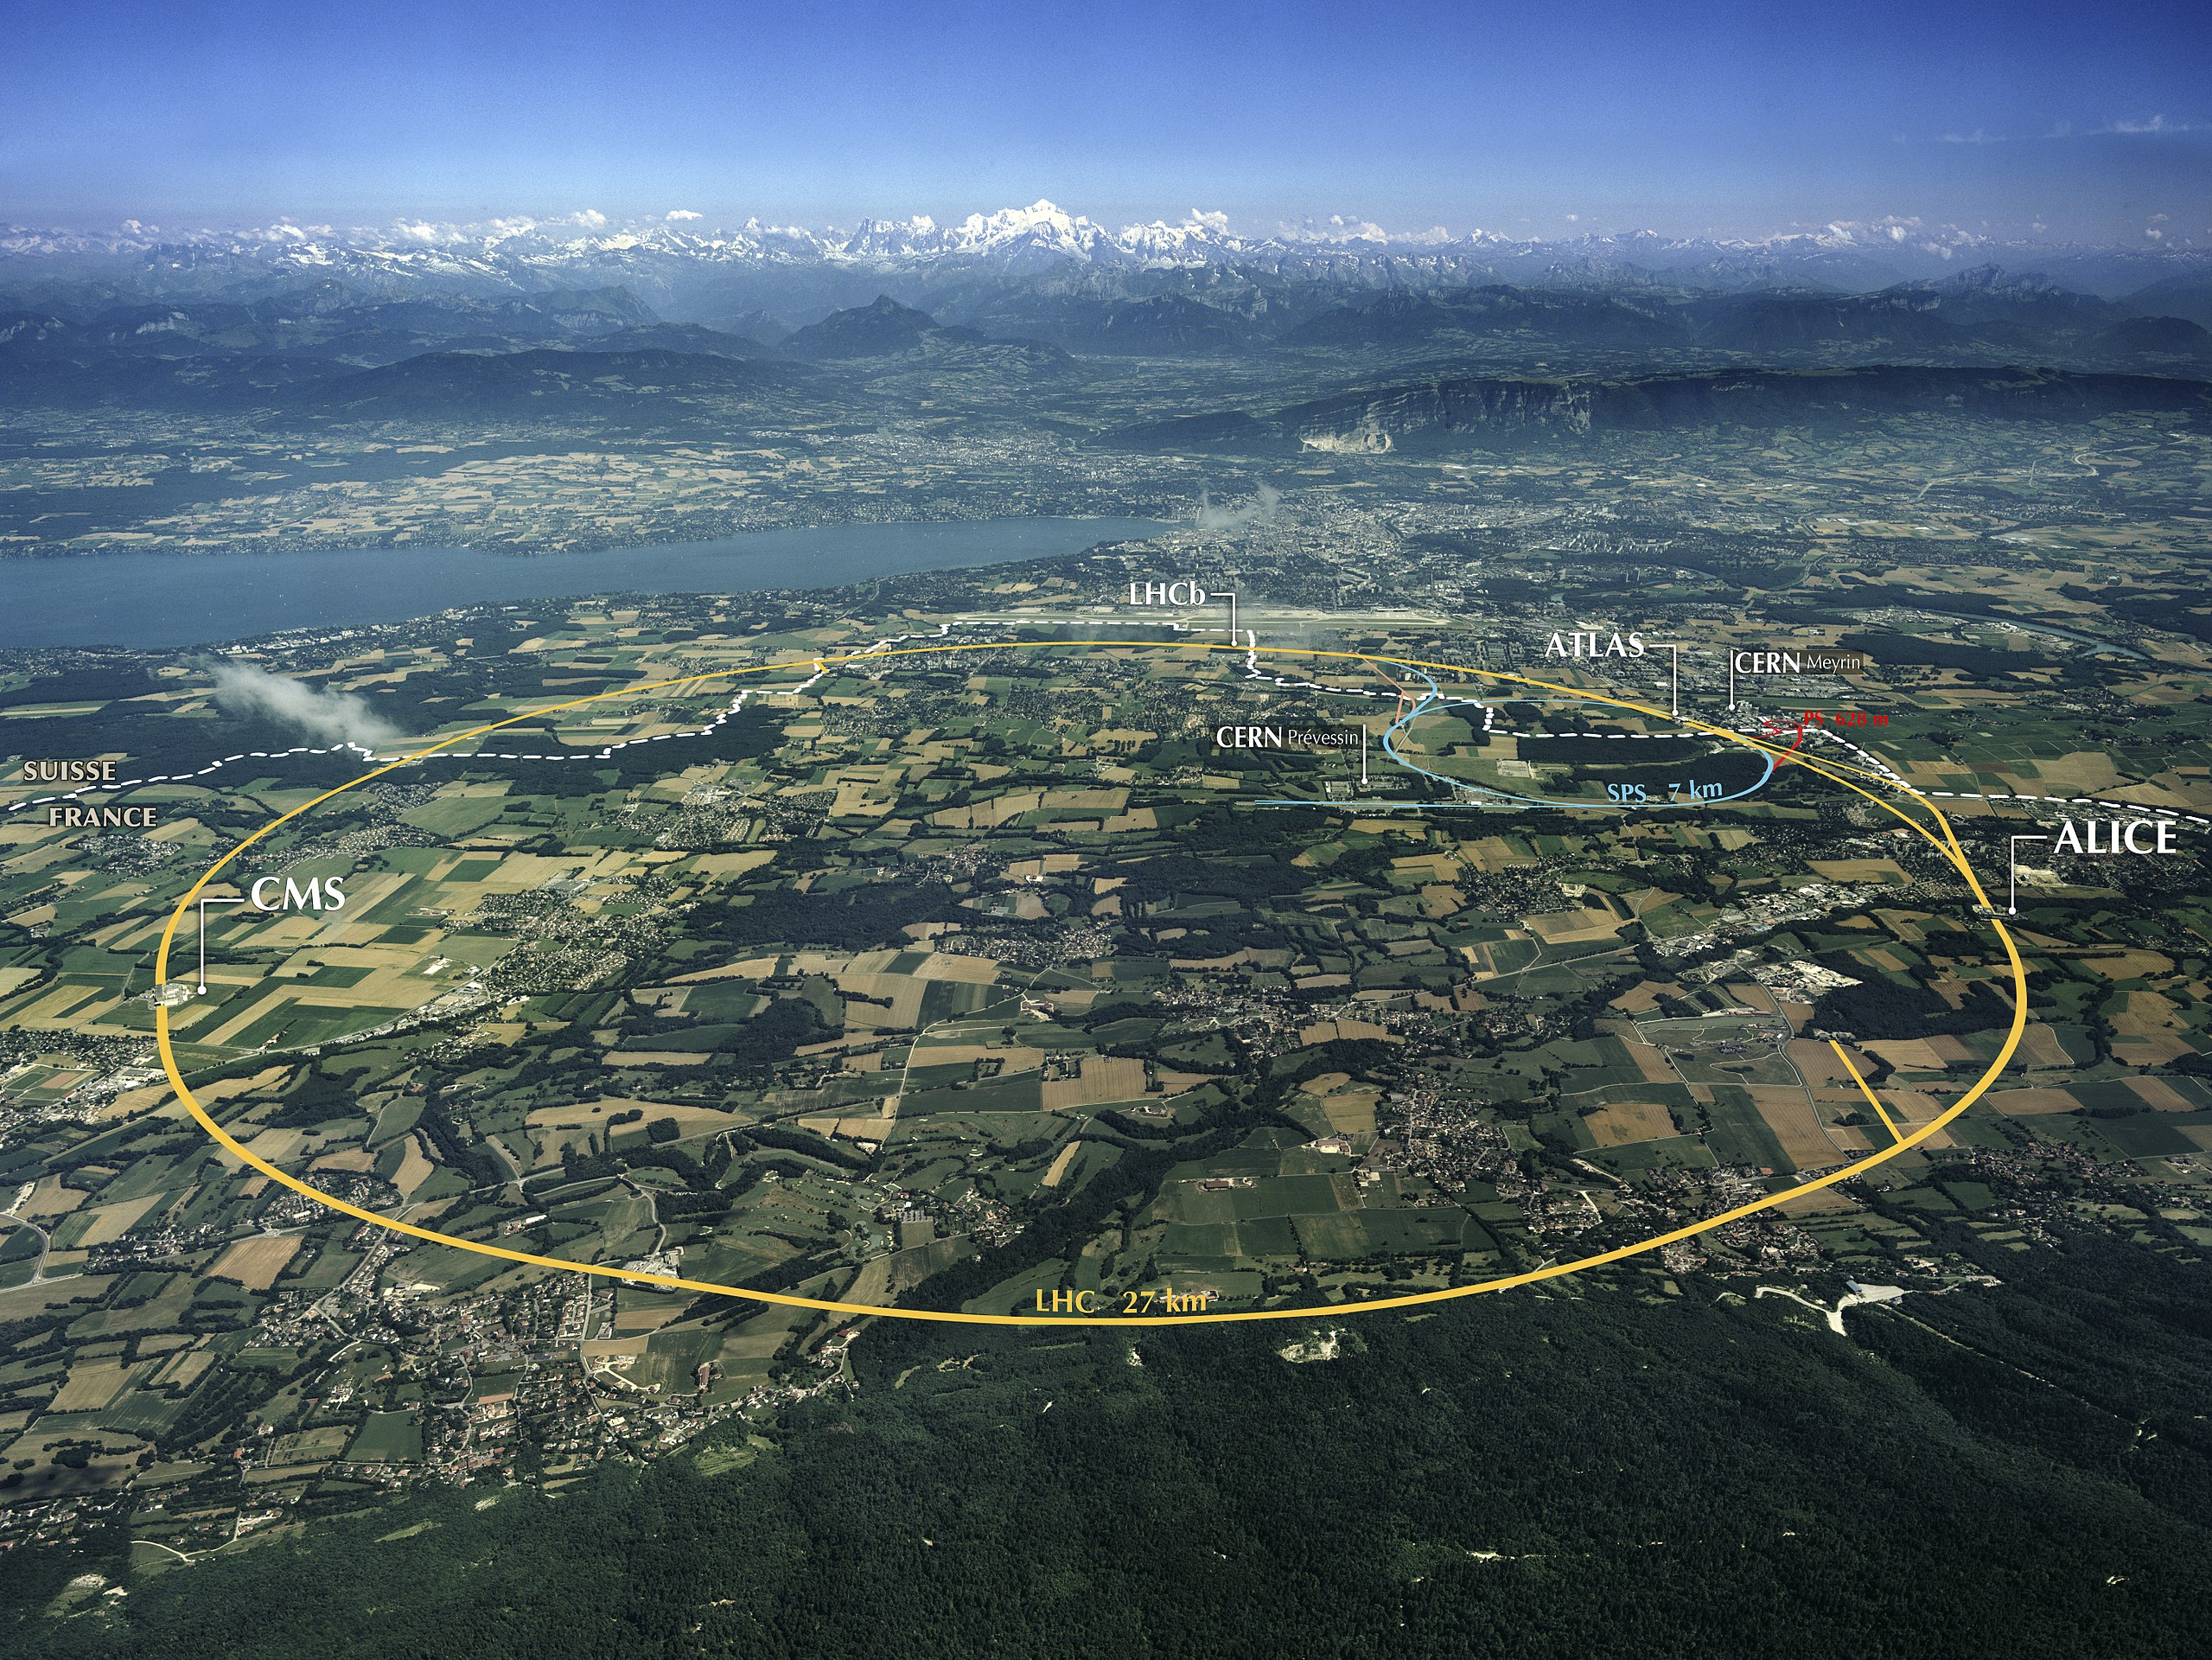
\includegraphics[width=0.45\textwidth,valign=c]{fig/lhc/cern_aerial_view.jpg}}
    \caption{
        A diagram illustrating the depth of the LHC beneath the surface (left), from Ref.~\cite{Servicegraphique:1708849}, and an aerial photograph of the entire CERN complex (right), from Ref.~\cite{Maximilien:1295244}. 
        The SPS and LHC tunnels illustrated in both figures. 
    }
    \label{fig:lhc_depth}
\end{figure}

\begin{figure}[htb]
    \centering
    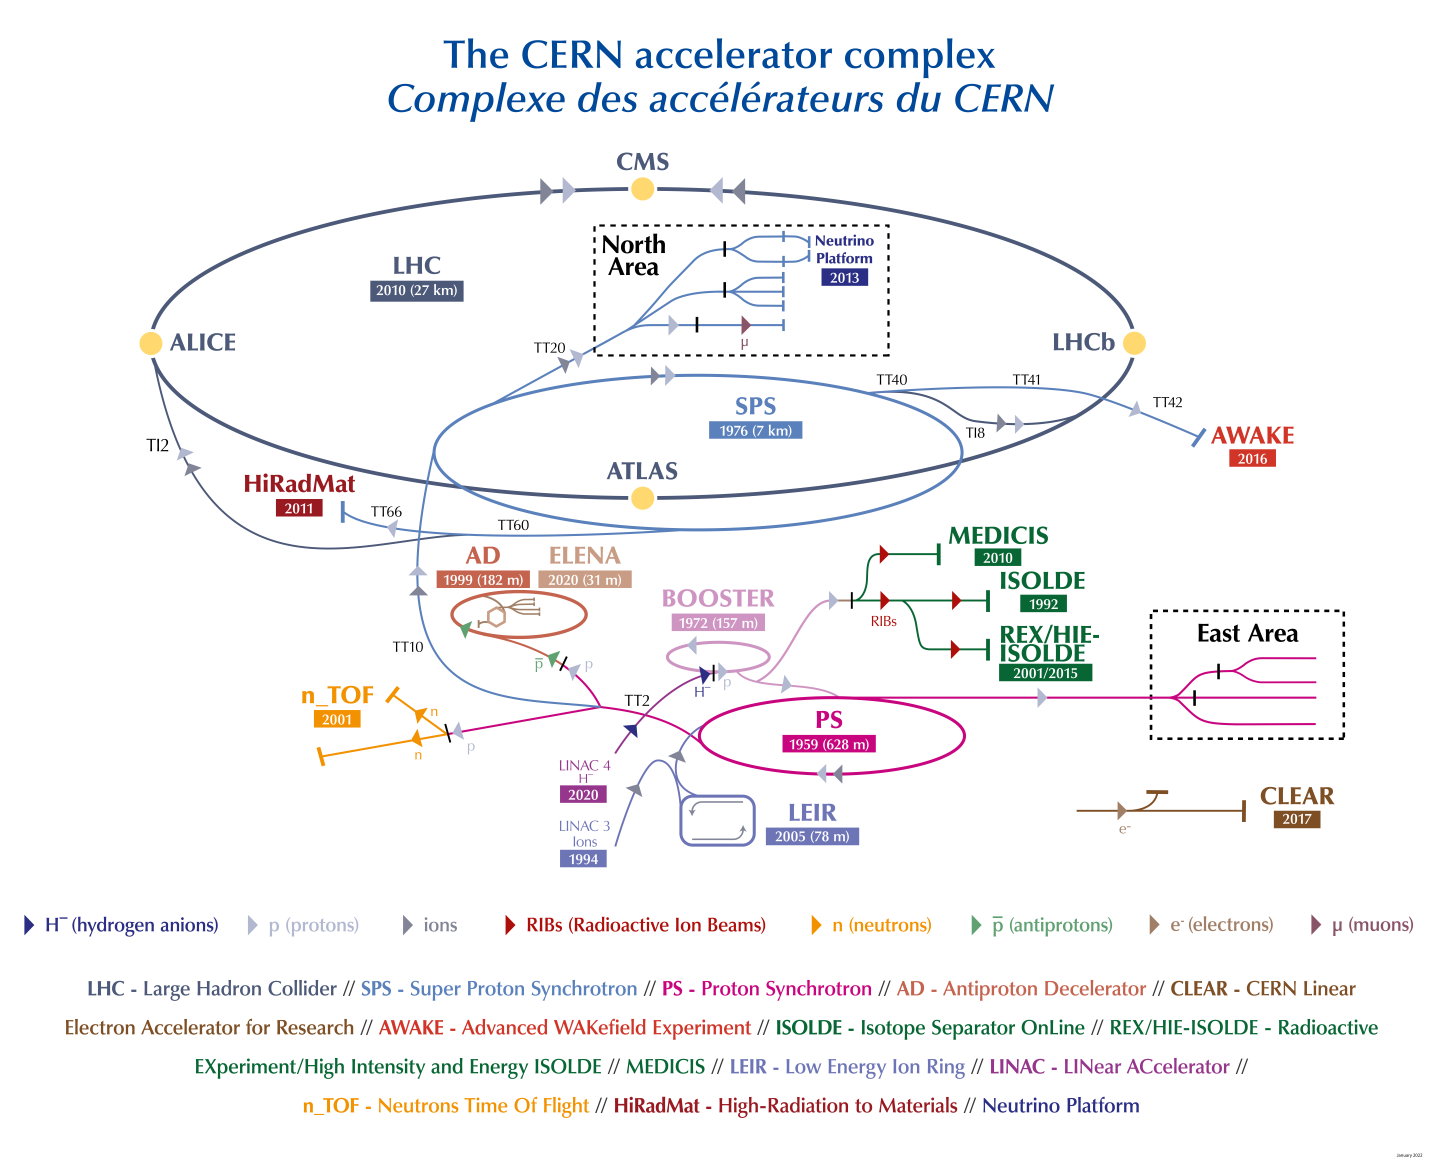
\includegraphics[width=0.95\textwidth]{fig/lhc/lhc_complex.png}
    \caption{
        The CERN complex illustrated in detail, from Ref.~\cite{Lopienska:2800984}. 
        The different stages of particle acceleration can be seen in detail, described here for protons. 
        First, negative hydrogen ions (H$^-$) generated by LINAC 4 are fed into BOOSTER, which strips the electrons from the H$^-$ ions, leaving only the protons, and accelerates them to 2\GeV. 
        Next, the Proton Synchrotron (PS) accelerates the protons to 26\GeV. 
        The PS feeds into the Super Proton Synchrotron (SPS) which further accelerates them to to 450\GeV. 
        Finally, the protons are fed into the LHC, which accelerates them to a final energy of 7\TeV. 
    }
    \label{fig:cern_complex}
\end{figure}

\begin{figure}[htb]
    \centering
    \subfloat{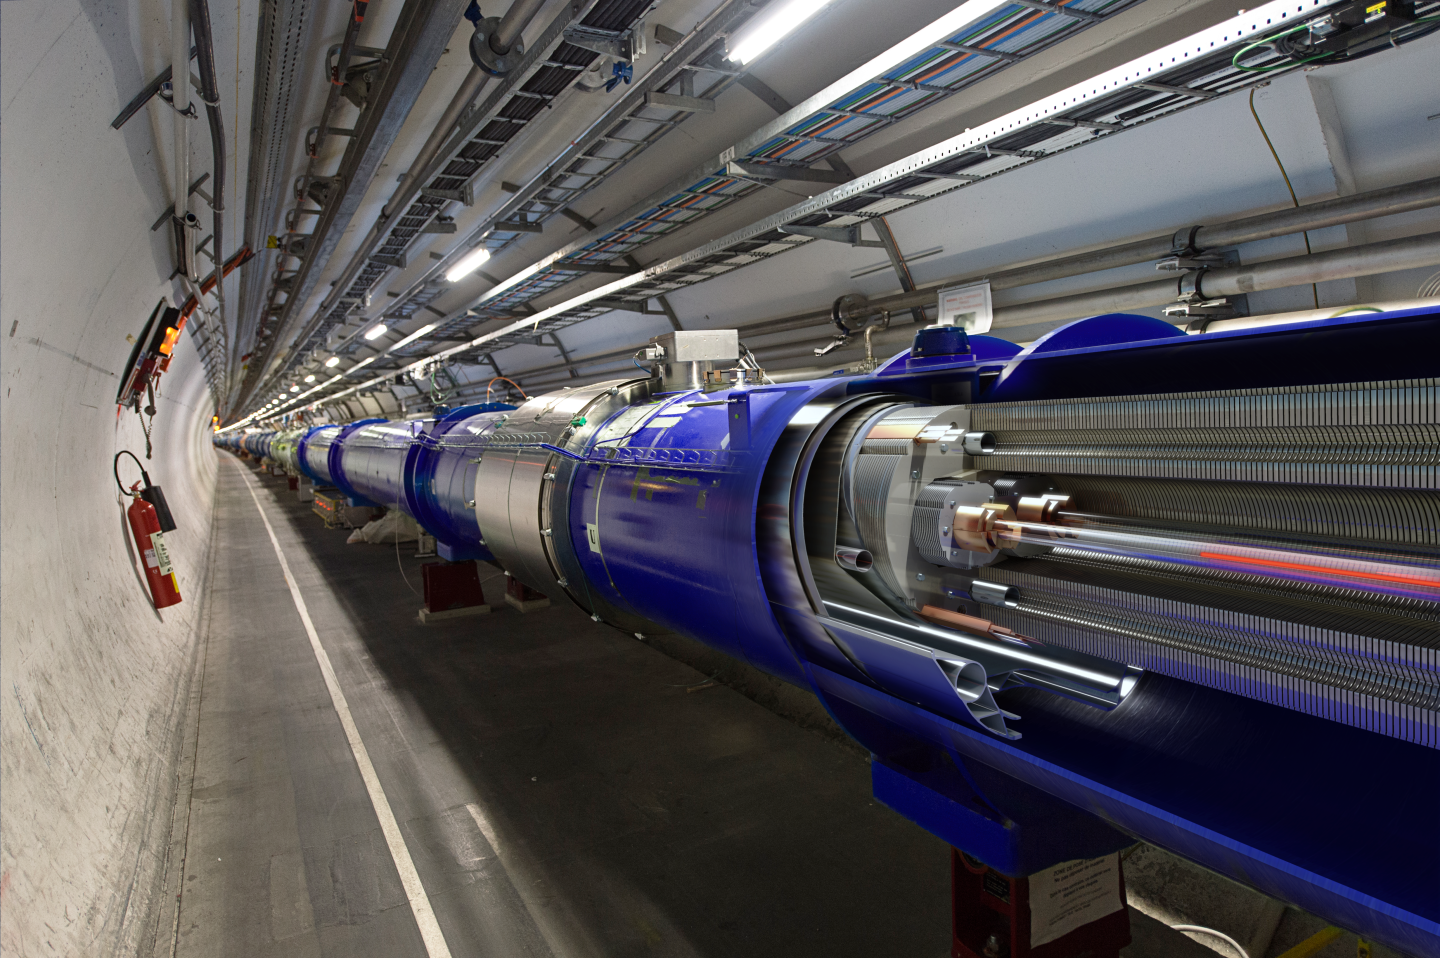
\includegraphics[width=0.475\textwidth,valign=c]{fig/lhc/dipole_cutaway.png}}\quad
    \subfloat{\includegraphics[width=0.425\textwidth,valign=c]{fig/lhc/dipole_jguiang.png}}
    \caption{
        A cutaway diagram illustrating the internals of a dipole magnet inside the LHC tunnel (left), from Ref.~\cite{Dominguez:1741036}, and a photograph of a decomissioned dipole magnet with a physicist for scale (right).
    }
    \label{fig:lhc_dipole}
\end{figure}

The protons are accelerated in bunches, composed of approximately 115 billion protons each, so when the bunches are brought together (called a ``bunch crossing''), over 200 billion protons are brought very close together.
However, only a small portion of them actually collide. 
During ``Run 2'' of the LHC from 2016 to 2018, for instance, there were 30 proton-proton (pp) collisions (e.g. Fig.~\ref{fig:normal_pu}) per bunch crossing on average, typically with only a single ``interesting'' collision (the ``primary vertex'') amongst them. % TODO: citation needed, plot or something of pileup needed
A collision is deemed interesting if it initiates a process that a physicist at the LHC wants to study (e.g. Fig.~\ref{fig:vbswh_feynman})---the non-interesting collisions are called ``pileup.'' 
To increase our odds of producing something truly interesting, the bunch crossings are spaced close together, with only 25 nanoseconds of separation. 
To put this into context, the speed of light is roughly 1 ft/ns, so the next bunch crossing will occur before the light from a screen on one side of the CMS control room can reach the eyes of someone standing on the other side (approximately 39 feet~\cite{CMSP5Layout}).
Therefore, particle detectors on the LHC must be capable of excellent resolution \textit{and} high throughput. 
That is, they must be able to resolve the particles from the primary vertex amongst the many others produced by the pileup, all within the 25 ns between bunch crossings. 

\subsection{Collision energy}
The collision energy, often written as $\sqrt{s}$, is measured in electronvolts (eV), the standard unit of energy in particle physics---more specifically, teraelectronvolts (TeV), or trillions of eV. 
In Run I of the LHC (2011--2012) the collision energy was ramped up to a maximum of 8\TeV, much lower than what the LHC was designed for. % TODO: citation needed
This was done out of an abundance of caution due to the fact that the LHC exploded when it was first turned on in 2008. % TODO: citation needed
Then, in Run II (2016--2018), the collision energy was increased to 13\TeV. 
Over the course of Run III, the collision energy will be ramped up to 14\TeV, where it will be held for the remainder of the LHC's lifetime (Fig.~\ref{fig:hl_lhc_timeline}). 

\subsection{Luminosity}
The luminosity ($\Lumi$) is measured in the inverse of the units of a cross section---inverse femptobarns ($\fbinv$), in particular. 
This allows for a quick calculation of how many pp collisions one can expect: simply multiply the lumonisity by the pp inelastic scattering cross section. 

\clearpage

\section{The Compact Muon Solenoid}
The Compact Muon Solenoid (CMS) Experiment is one of two general purpose LHC experiments, the other being the ATLAS\footnotemark{} Experiment, among the four major experiments supported by the LHC~\cite{LHCWeb}, where the other two are more specialized: ALICE, for studying heavy ion collisons, and LHCb, for studying b quarks. 
\footnotetext{Whereas ATLAS is, putting it politely, a rather creative acronym: ``A Toroidal LHC ApparatuS.''}
Compared to ATLAS, which stands at a mighty $46\times25\times25$ meters in dimension, CMS is ``compact'' at a stout $21\times15\times15$ m, with a dedicated muon system and one of the world's largest solenoid magnets~\cite{ATLASWeb, CMSWeb}. 
See Fig.~\ref{fig:cms_labeled} for its exact specifications, and Figures~\ref{fig:cms_pics} and \ref{fig:cms_jguiang} for some beauty shots. 

\begin{figure}[htb]
    \centering
    \includegraphics[width=0.9\textwidth]{fig/cms/cms_labeled.jpg}
    \caption{
        A detailed cutaway diagram of CMS, with each subdetector labeled with its name and some its characteristics, from Ref.~\cite{Sakuma:2665537}. 
    }
    \label{fig:cms_labeled}
\end{figure}

\begin{figure}[htb]
    \centering
    \subfloat{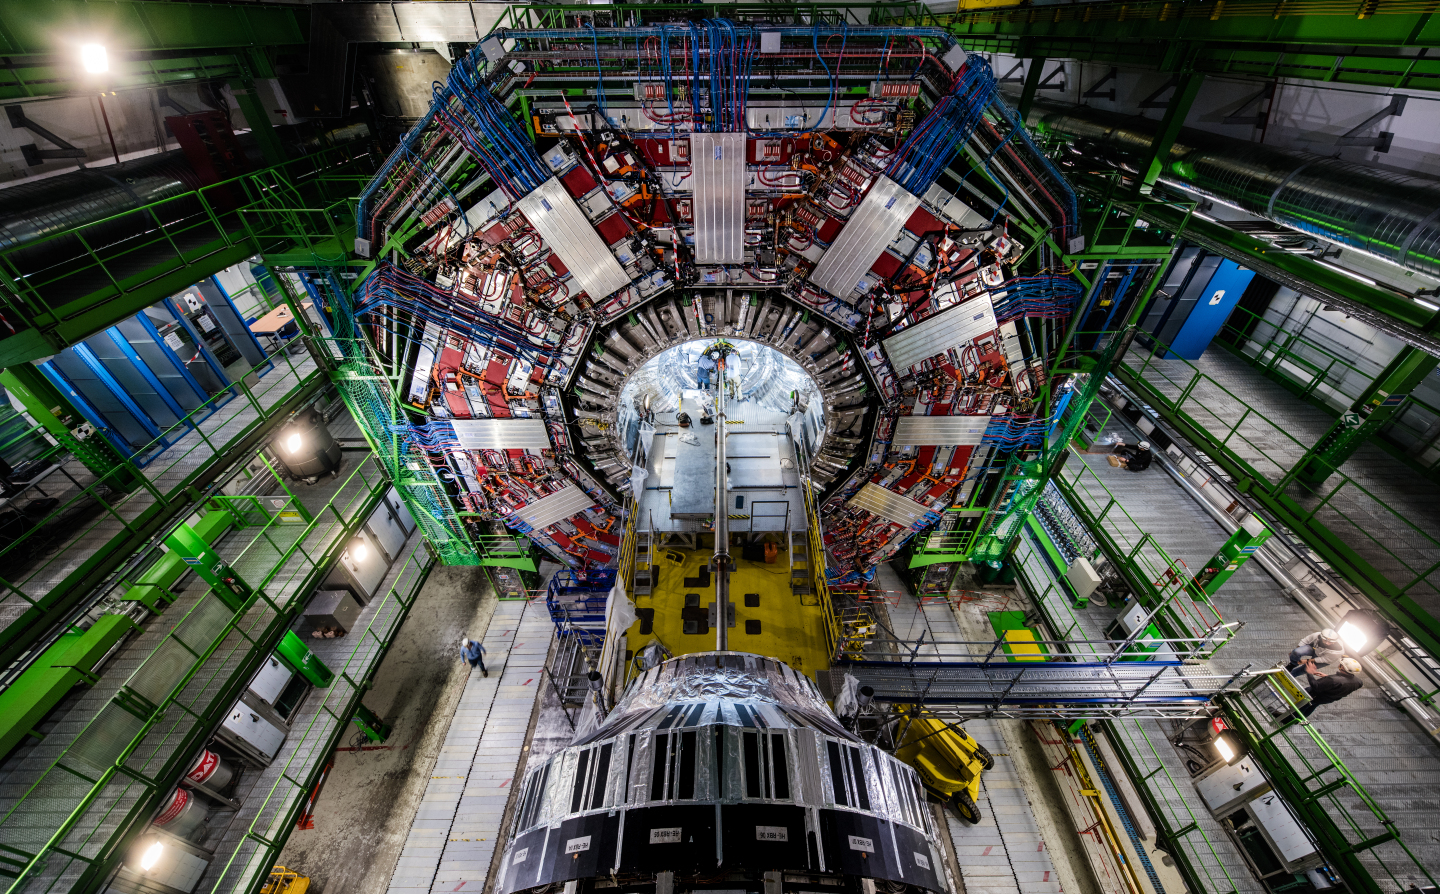
\includegraphics[width=0.465\textwidth]{fig/cms/cms_picture1.jpg}}\quad
    \subfloat{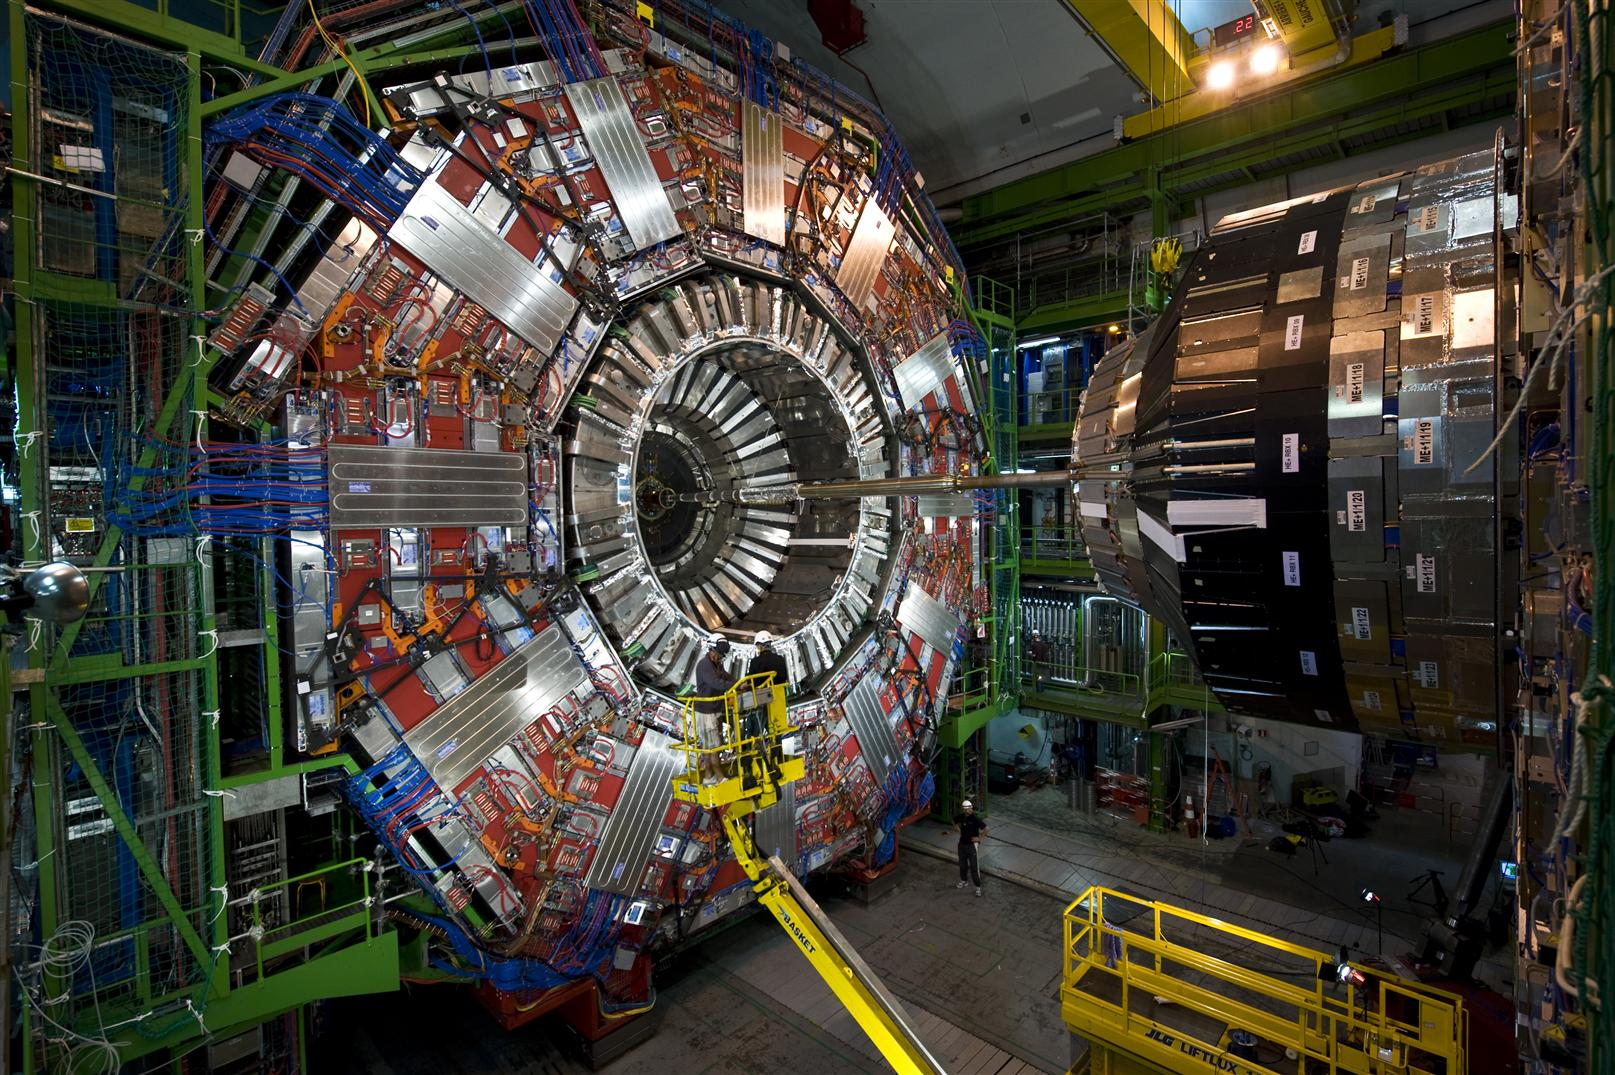
\includegraphics[width=0.435\textwidth]{fig/cms/cms_picture2.jpg}}
    \caption{
        The Compact Muon Solenoid in all of its glory, with one of the endcaps separated from the main body of the experiment, pictured from the top (left) and side (right). 
    }
    \label{fig:cms_pics}
\end{figure}

\begin{figure}[htb]
    \centering
    \subfloat{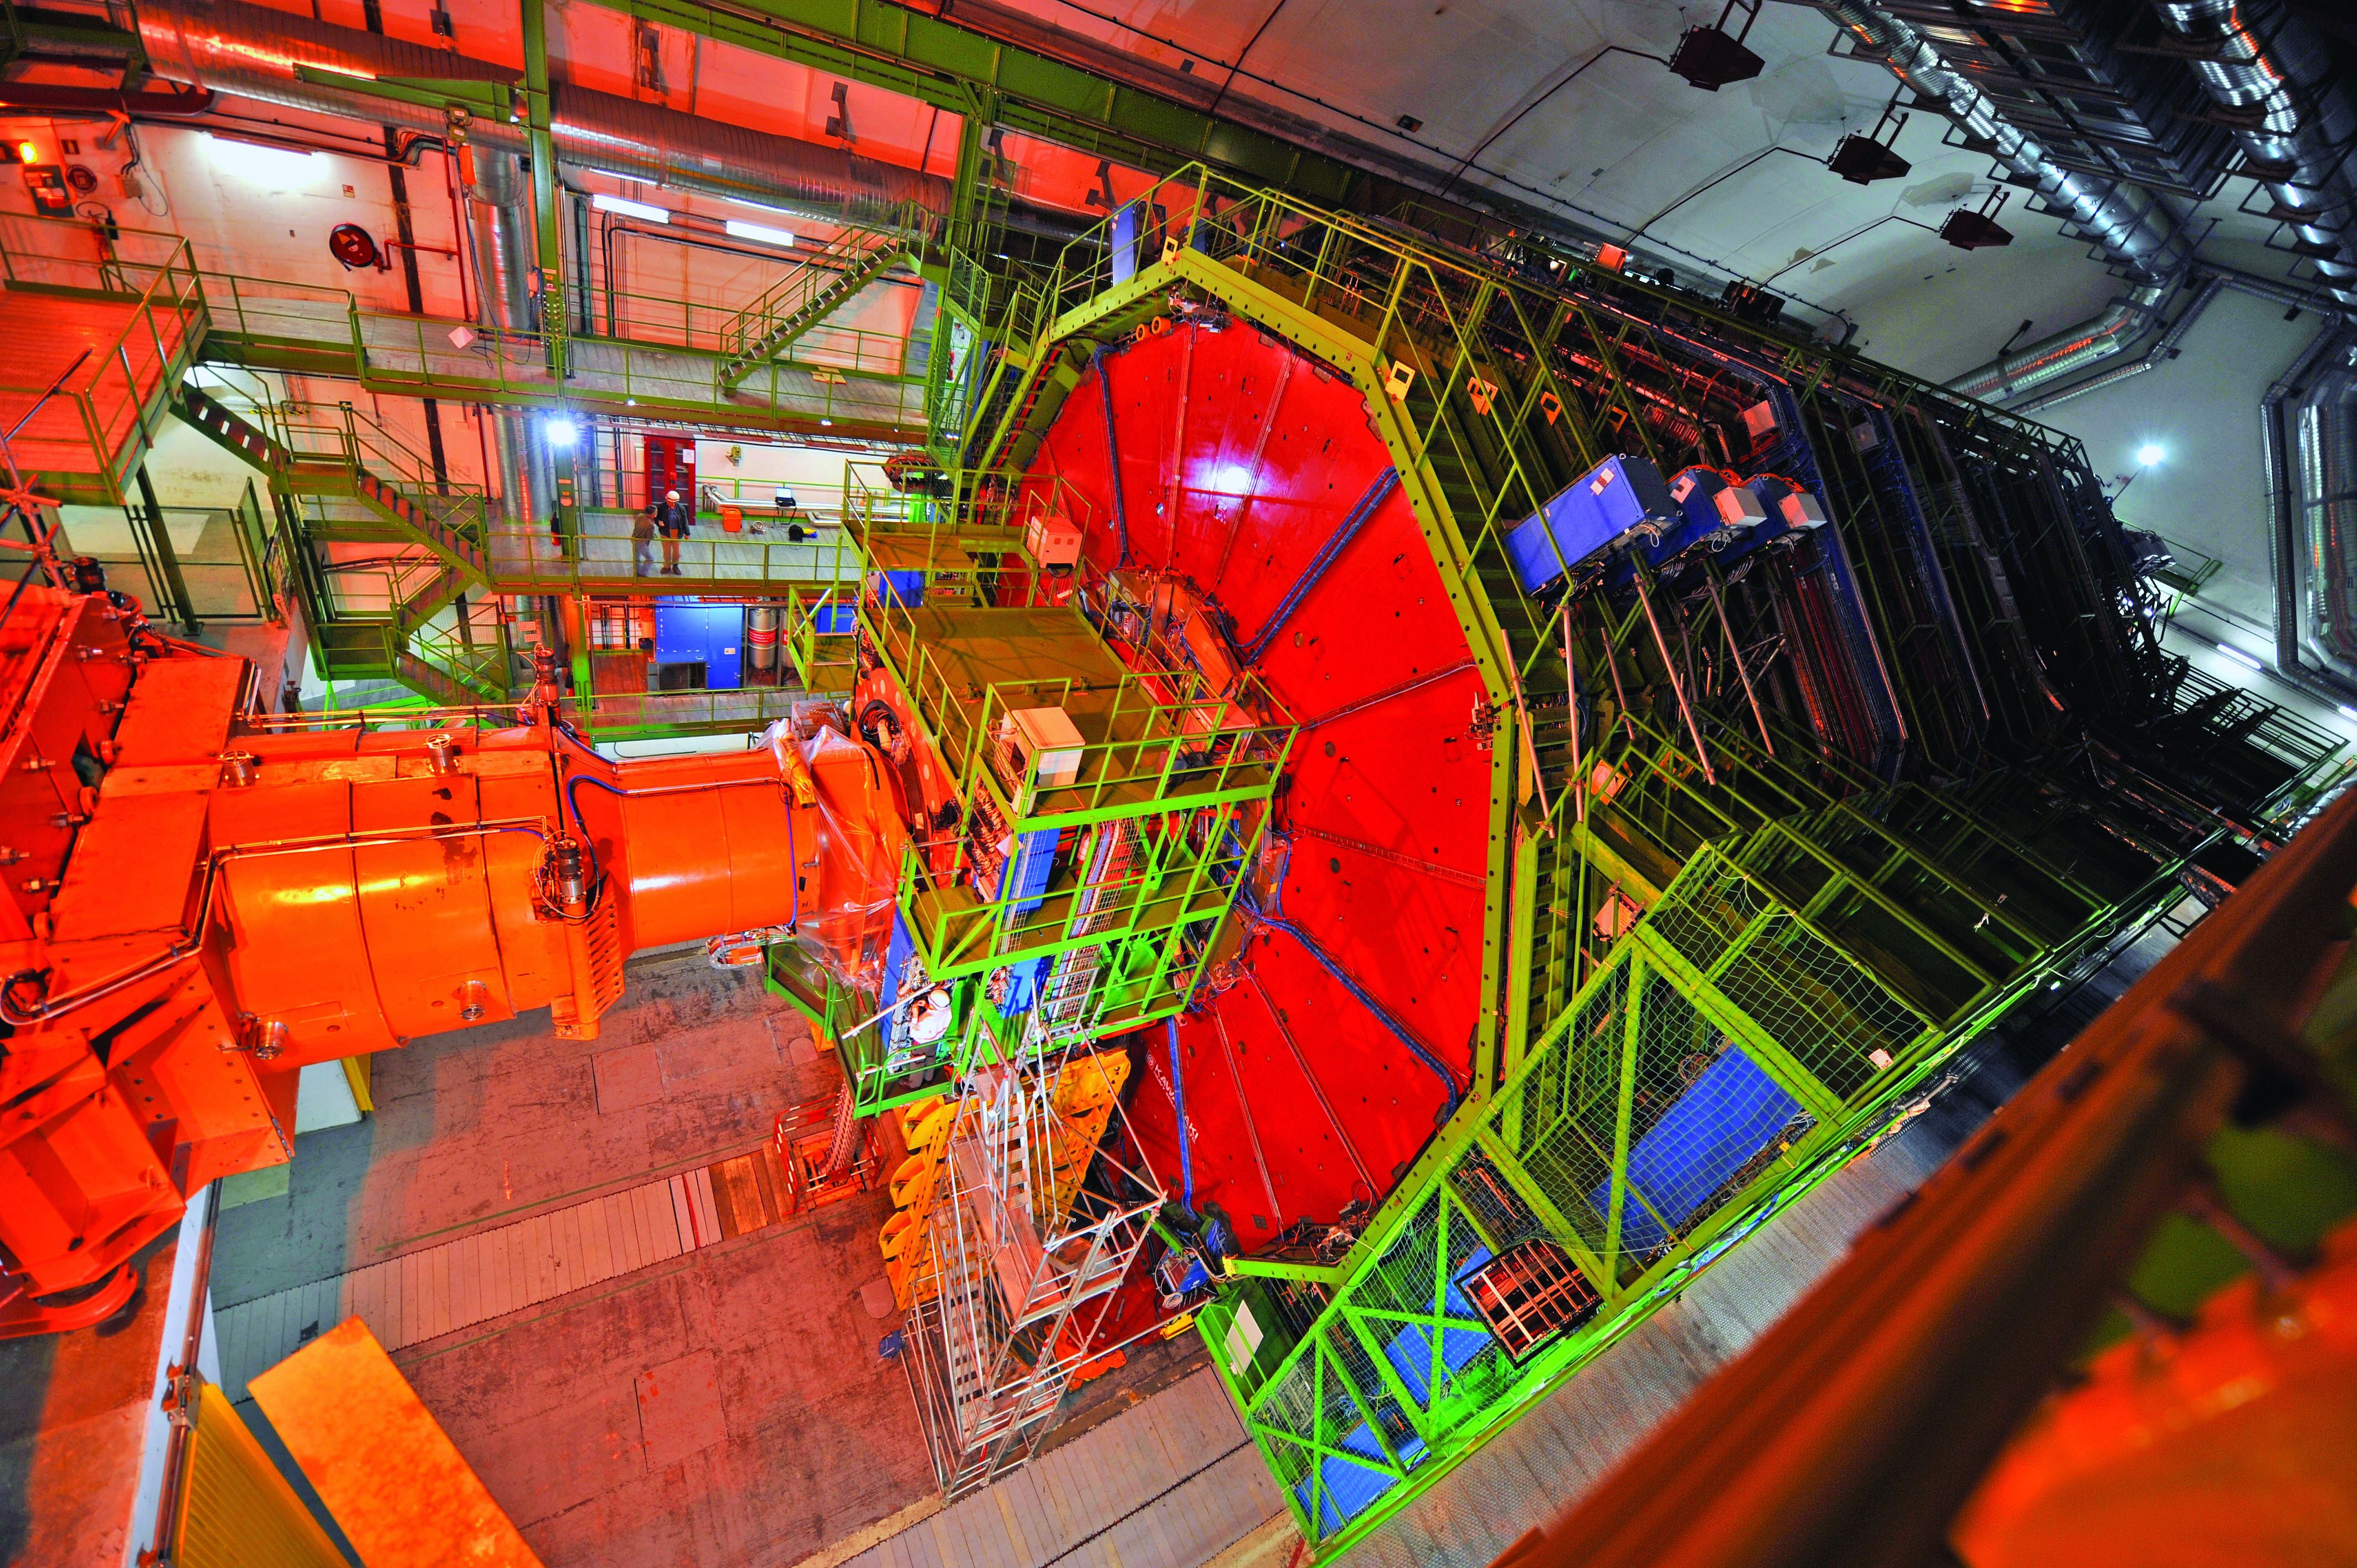
\includegraphics[width=0.492\textwidth,valign=c]{fig/cms/cms_picture3.jpg}}\quad
    \subfloat{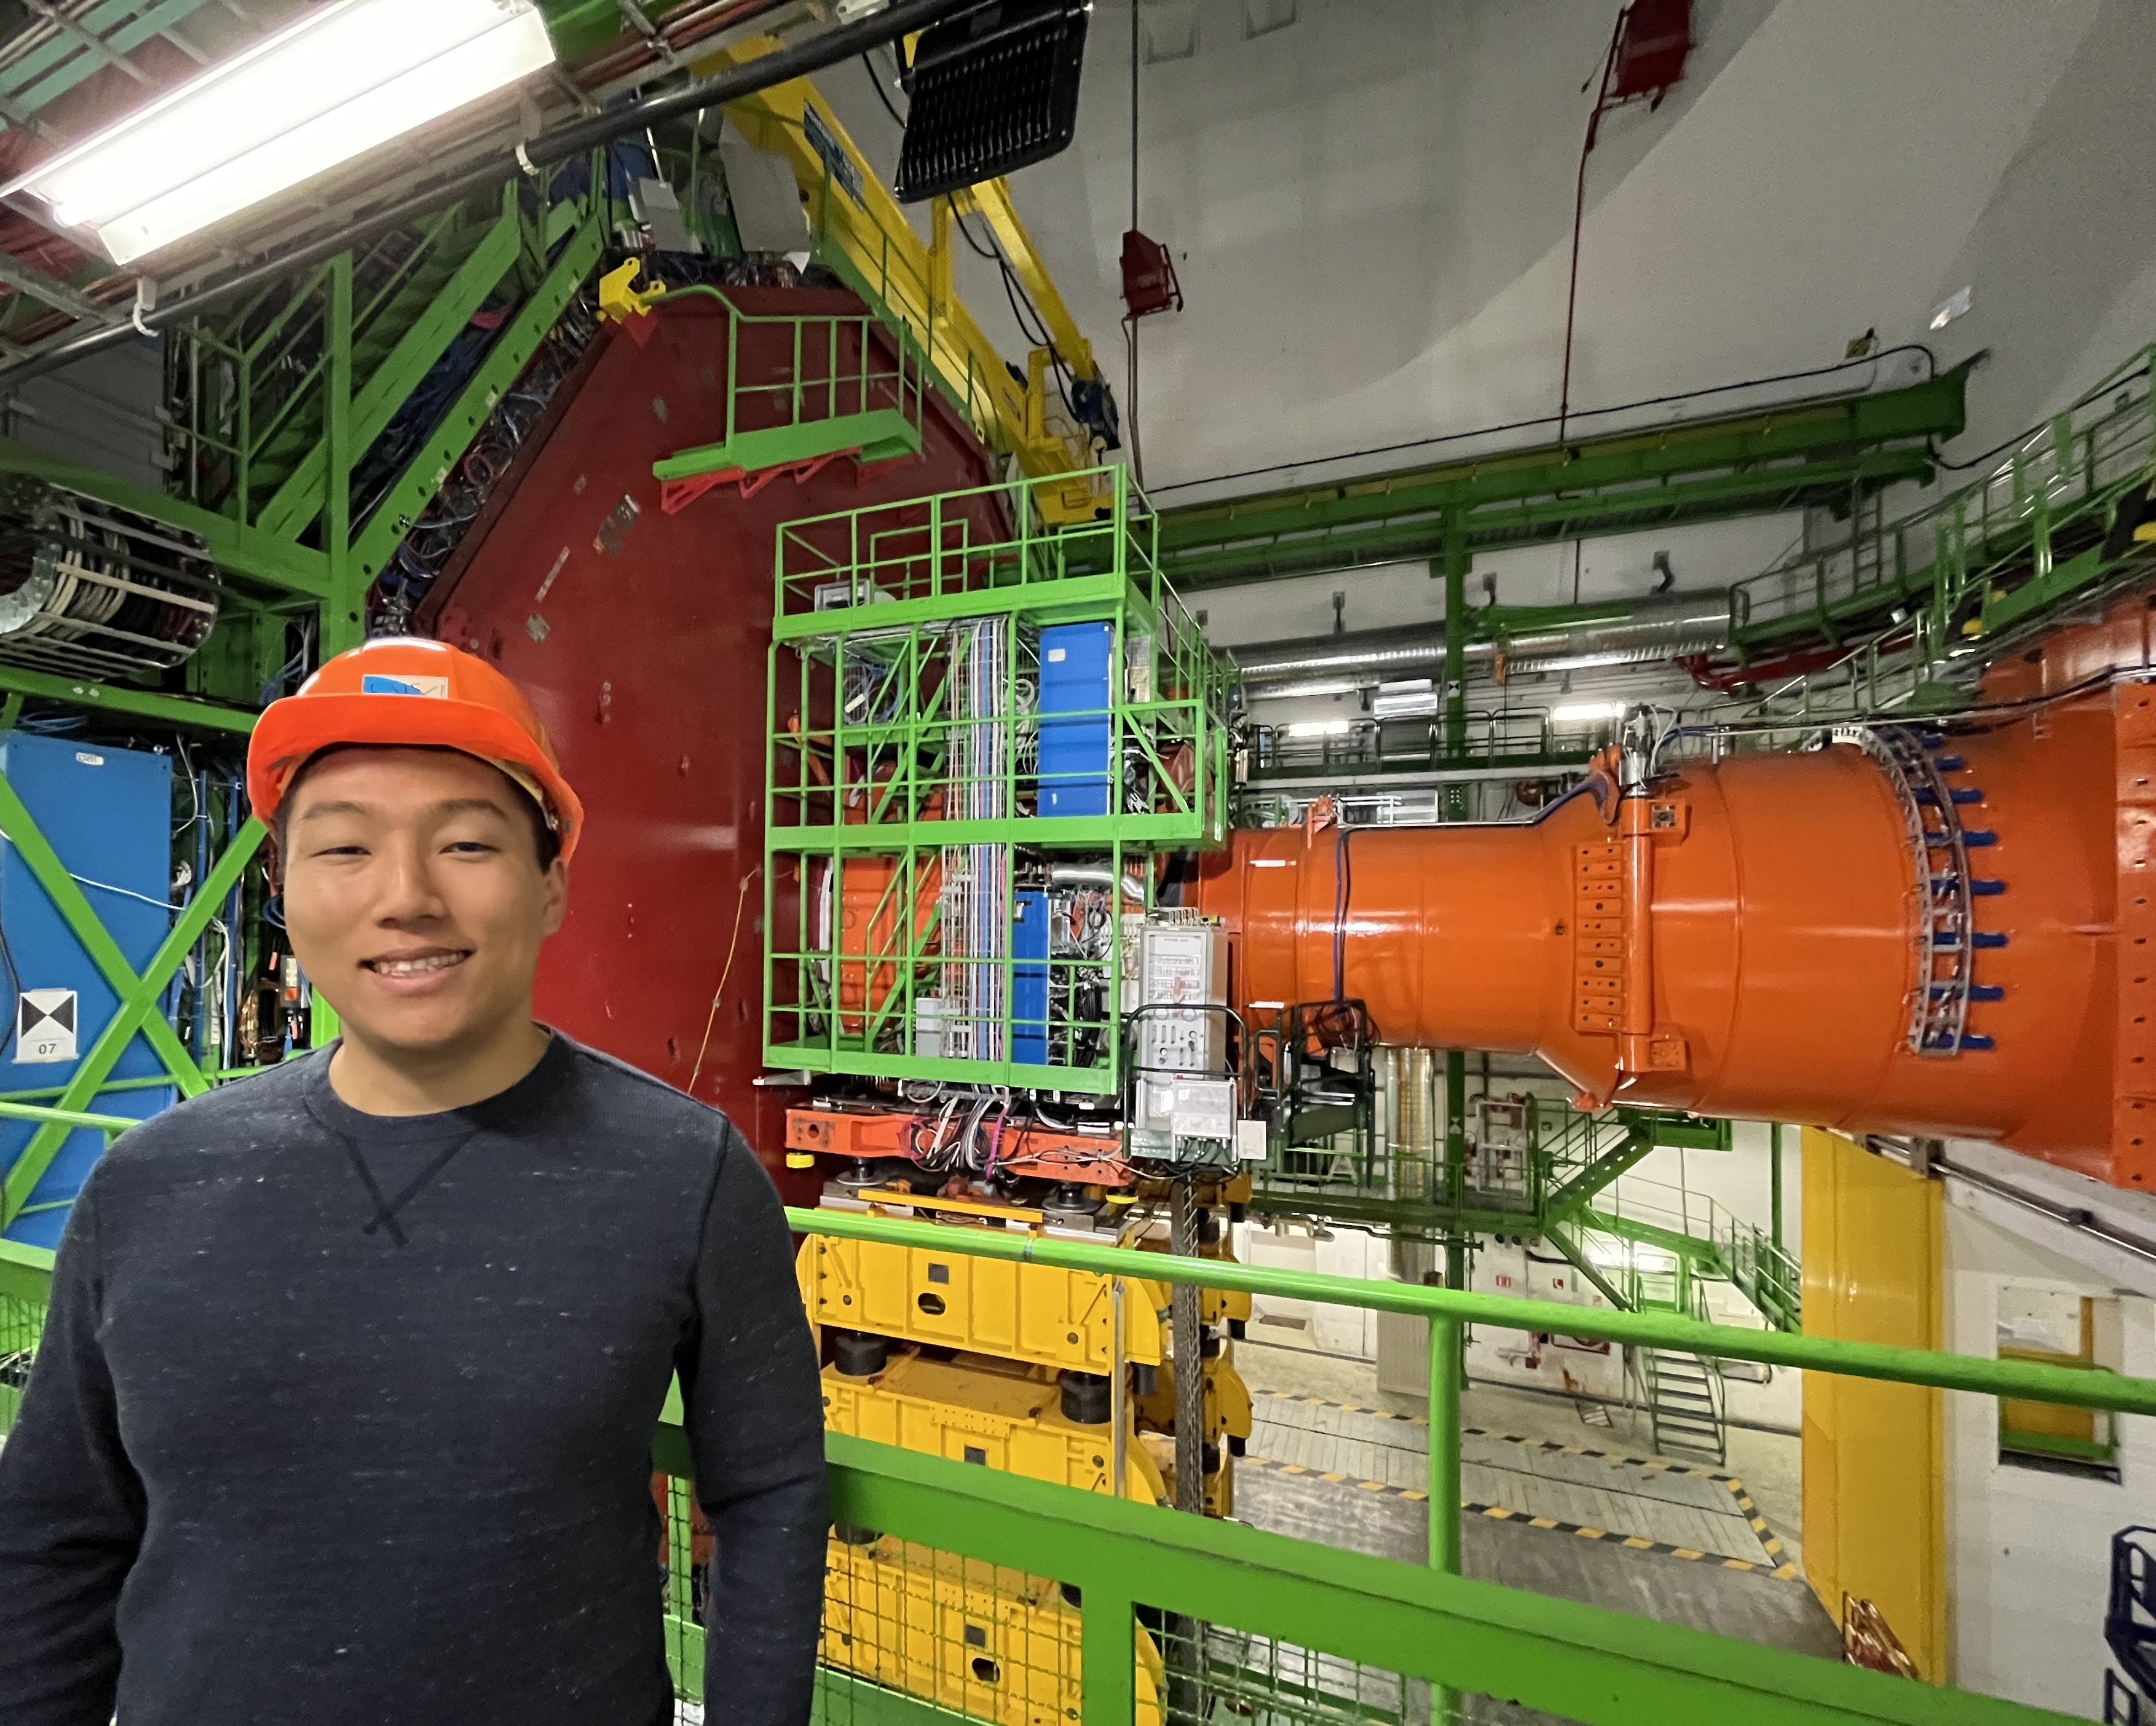
\includegraphics[width=0.408\textwidth,valign=c]{fig/cms/cms_jguiang.jpg}}
    \caption{
        The Compact Muon Solenoid in the closed configuration, pictured from the top (left) and side, with a physicist in the foreground for scale (right).
    }
    \label{fig:cms_jguiang}
\end{figure}

\subsection{Overview}
The CMS Experiment is composed of subdetectors arranged in layers, where each layer interacts with or completely absorbs certain particles, producing an electric signal that can be used to measure some property of those particles. 
The innermost layer is the silicon tracker, which allows for the reconstruction of the trajectories of throughgoing charged particles (``tracks''). 
Next is the electromagnetic calorimeter (ECAL), which absorbs electrons and photons and records their individual energies. 
After the ECAL, there is the hadronic calorimeter (HCAL), which instead absorbs hadrons and records their individual energies. 
These first three layers---the tracker, ECAL, and HCAL---are surrounded by the eponymous superconducting solenoid, which immerses them in an approximately uniform magnetic field that runs parallel to the beamline. 
This is critical: charged particles fly along curved trajectories in a magnetic field according to their charge and momentum, so those properties can be inferred from a high-quality measurement of each particle's trajectory. 
Finally, there are alternating layers of muon chambers, the other half of the experiment's namesake, and iron support structures. 
The former detects throughgoing muons, which pass through all of the inner layers mostly unperturbed, and measures an additional portion of their tracks.
However, the latter is equally important: the iron ``return yoke'' guides the magnetic field outside of the solenoid, absorbs stray particles that make it past the inner layers, and supports the immense weight of CMS itself. 
By combining information from all of these detectors, the exact identity of any individual particle can, in principle, be inferred based on which detectors registered a signal. 
Therefore, a full ``picture'' of each pp collision event is recorded by CMS for further study. 
The exact function of each subdetector layer described here is detailed below.

\subsection{Superconducting solenoid}
The curve of a track is critical, as it allows us to infer the charge and momentum of a particle. 
However, in a weak magnetic field, the particles produced at the LHC would have nearly straight tracks, due to the large pp collision energy. 
The magnetic field inside of CMS must therefore be very large~\cite{CMSWebMagnet}. 
It should also be nearly uniform everywhere in order to make the determination of each particle's charge and momentum as simple as possible. 
The CMS magnet must also be large in dimension, however, as it must surround the tracker, ECAL, and HCAL, since it would otherwise block outgoing particles. 

By winding copper wire into a helix and passing a current through it, we can generate an magnetic field whose strength is directly proportional to the current and number of turns of the wire, but inversely proportional to the length of the helix. 
Within the volume of the helix, the magnetic field will be almost uniformly oriented in a single direction, determined by the orientation of the helix and direction of the current (Fig.~\ref{fig:cms_magnet_ideal}). 
This is not true outside of the helix where the magnetic field lines curve in space. 

\begin{figure}[htb]
    \centering
    \subfloat[]{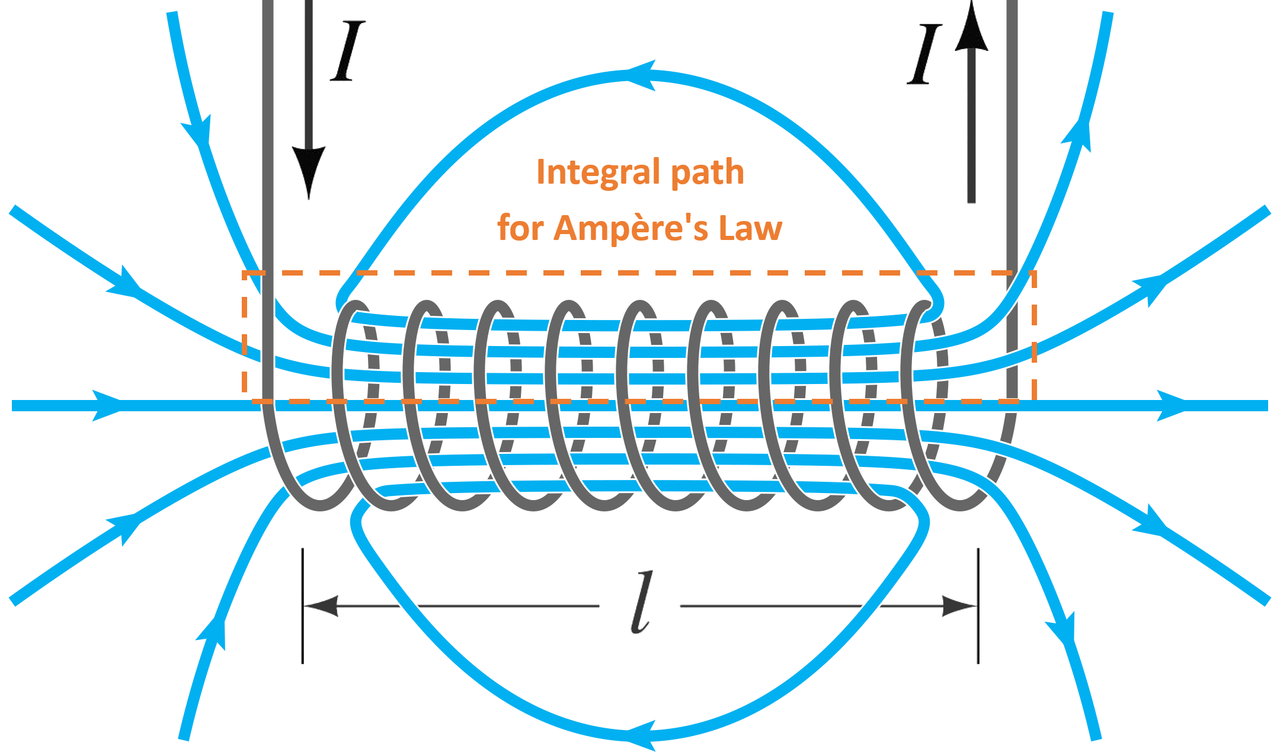
\includegraphics[width=0.4\textwidth,valign=c]{fig/cms/solenoid_ideal.png}\label{fig:cms_magnet_ideal}}\quad
    \subfloat[]{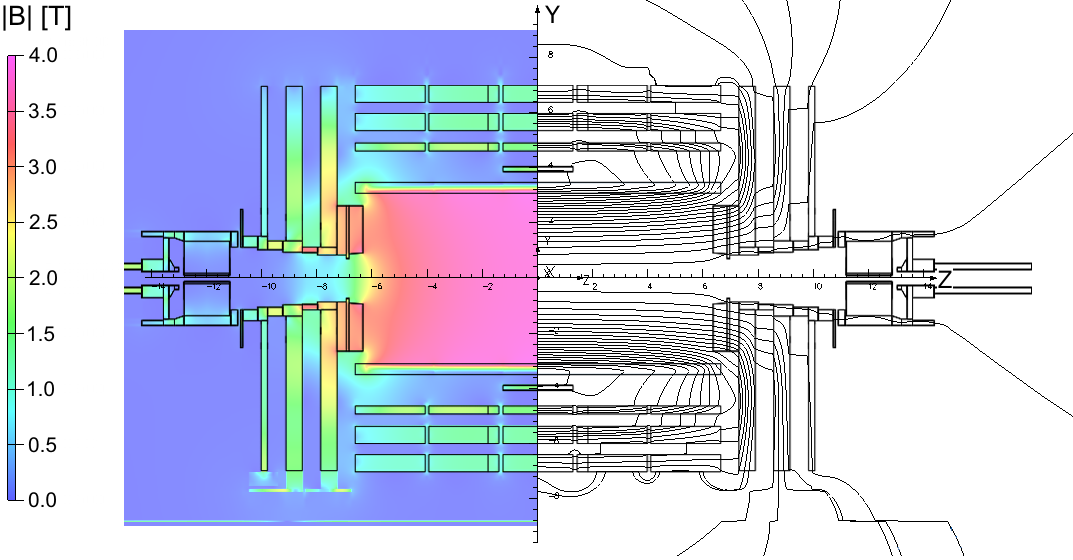
\includegraphics[width=0.5\textwidth,valign=c]{fig/cms/solenoid_field.png}\label{fig:cms_magnet_field}}
    \caption{
        The field lines of an ideal solenoid (a) and those of the CMS magnet (b), from Ref.~\cite{CMS:2009moq}. 
        For the ideal solenoid, the magnetic field is described by a simple equation: $B = \mu_0\frac{NI}{l}$, where $\mu_0$ is the magnetic constant, $N$ is the number of turns, $I$ is the current, and $l$ is the length of the helix. 
    }
    \label{fig:cms_fields}
\end{figure}

The CMS magnet~\cite{CERN-LHCC-97-010} is a massive\footnotemark{} realization of a solenoid. 
\footnotetext{It was built offsite, however, so it needed to be designed to fit within 7 such that it could be wheeled through the streets in Cessy, France (under which CMS is situated)~\cite{CMSWebMagnet}.}
It is comprised of over 2000 turns of Rutherford wire, which has a rectangular cross section (Fig.~\ref{fig:cms_magnet}). 
In operation, it is cooled to superconducting temperatures (-268.5 \de{}C, or one degree warmer than outer space), such that a high current of 20 kiloamperes\footnotemark{} can be passed through the coil without destroying it. 
\footnotetext{For scale, this is 100\,000 times larger than the minimum fatal current for humans (100--200 milliamperes)~\cite{10.1093/ptj/46.9.968}.}
This configuration allows the CMS magnet to produce a mostly uniform magnetic field of 4 T inside of the solenoid volume. 
That is 2--4 times larger than an MRI, which are typically 0.5--1.5 T~\cite{Berger2002-gs}, within a volume that is 1000 times larger. % TODO: citation needed for volume of an MRI?
We must also, however, have a fairly uniform magnetic field outside of the solenoid in order to maintain good momentum resolution for muons. 
To achieve this, the iron support structures that hold CMS together are also designed to guide the magnetic field lines (Fig.~\ref{fig:cms_magnet_field}). 
Inside of the iron, the magnetic field runs almost uniformly parallel to the field inside of the solenoid, but in the opposite direction---this gives muon tracks a characteristic S-shape in the transverse plane. 

\begin{figure}[htb]
    \centering
    \subfloat{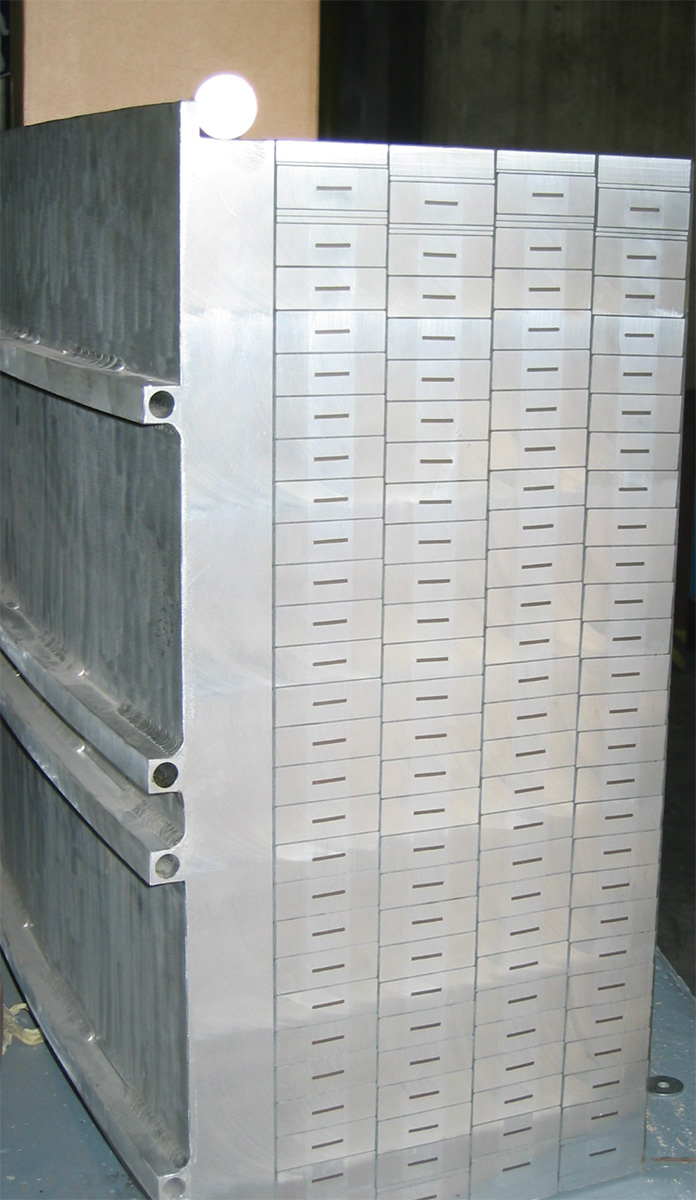
\includegraphics[width=0.3\textwidth,valign=c]{fig/cms/solenoid_wedge.jpg}}\quad
    \subfloat{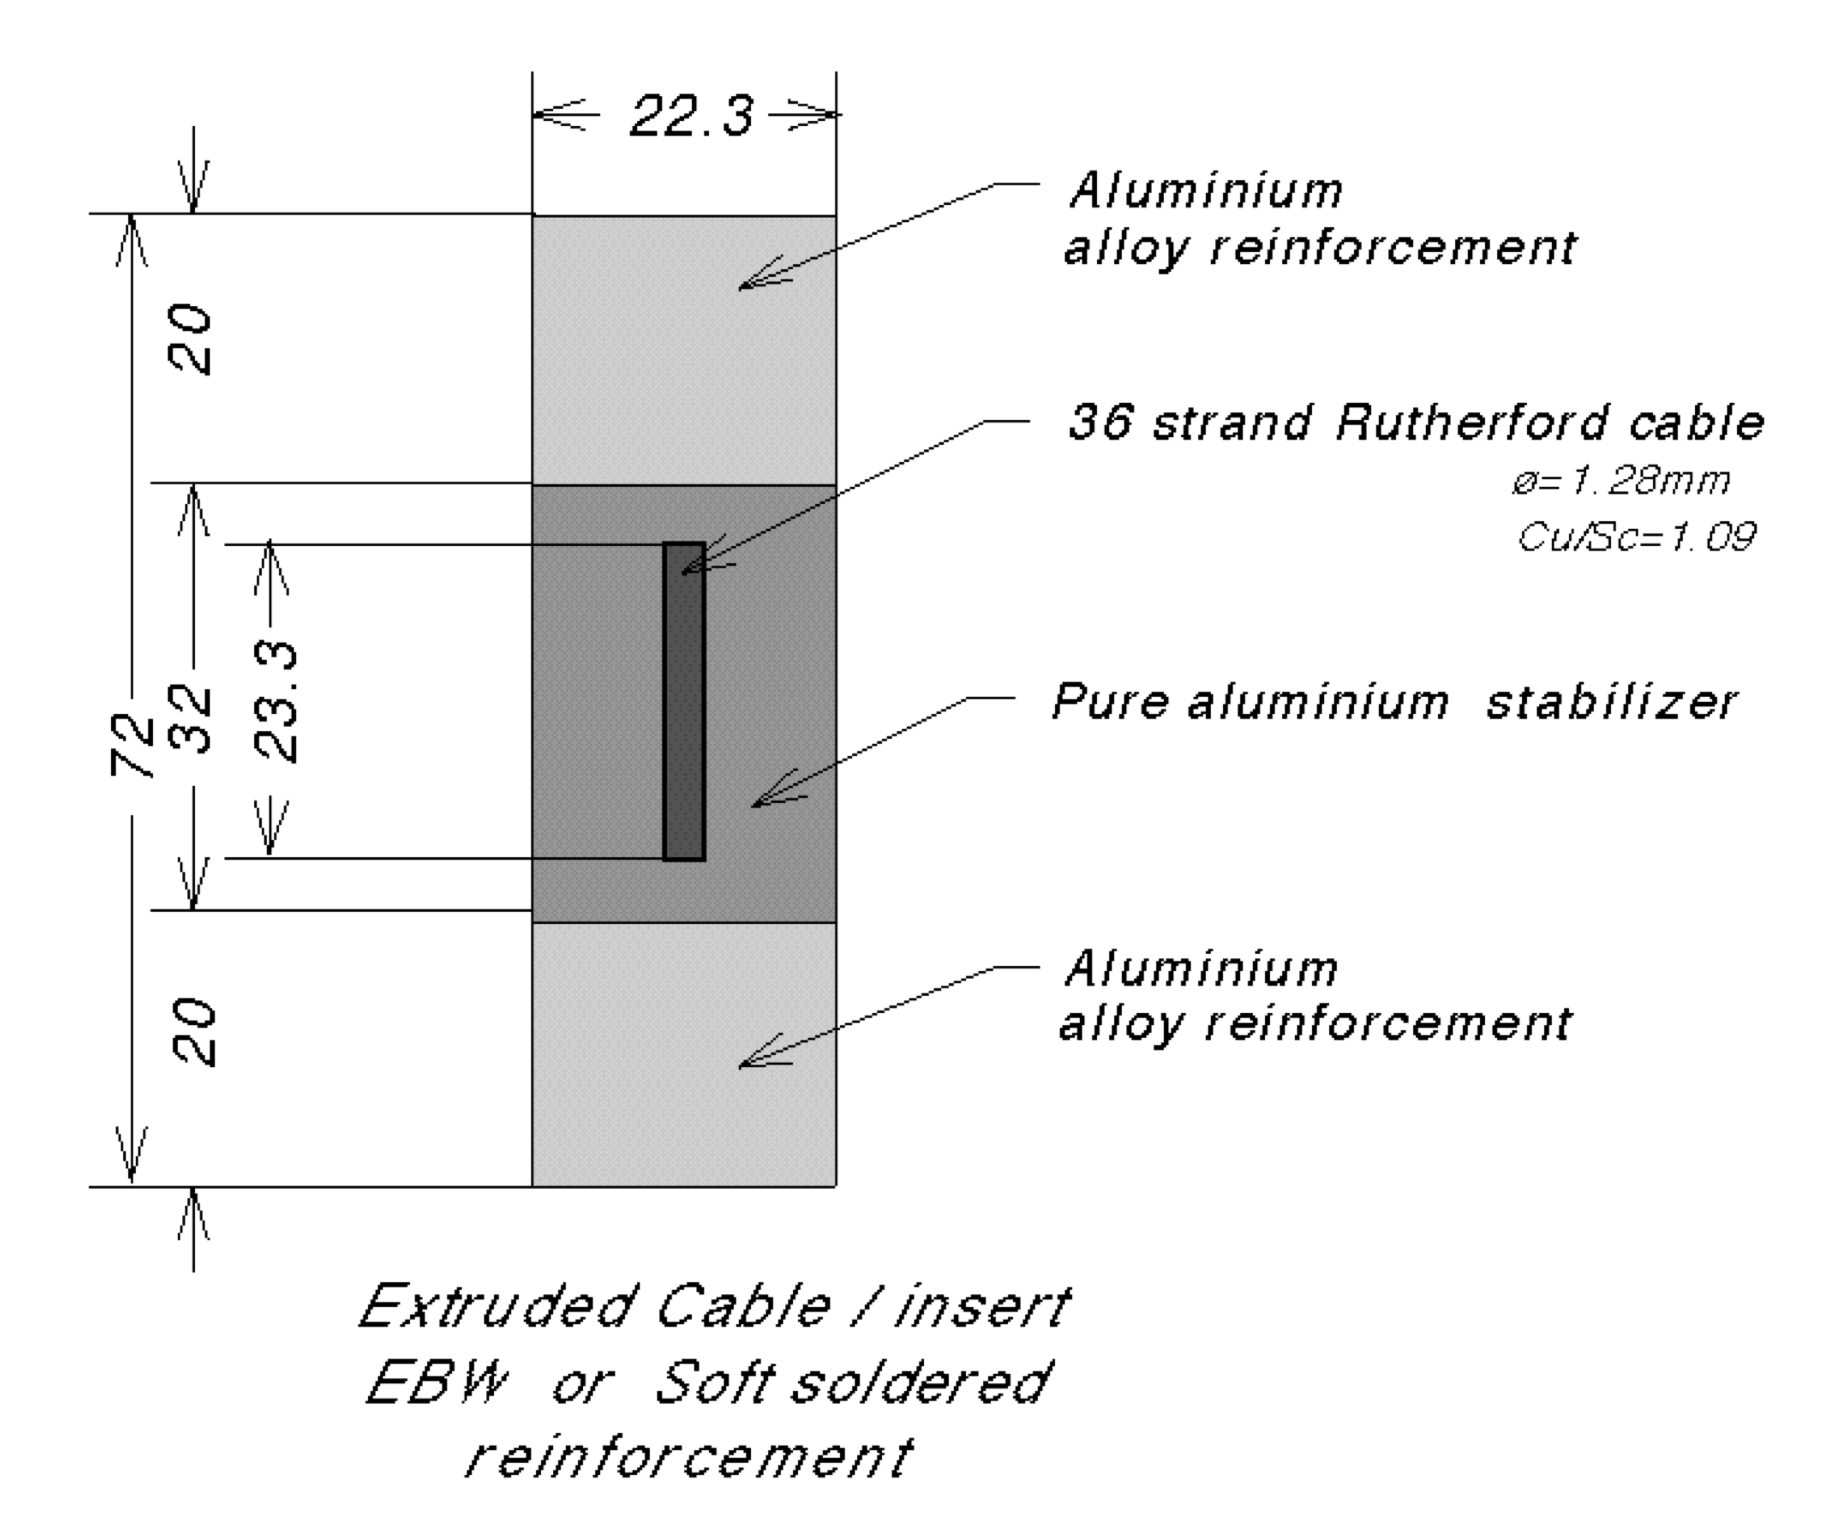
\includegraphics[width=0.6\textwidth,valign=c]{fig/cms/solenoid_cable.png}}
    \caption{
        A photograph of a section of the CMS magnet, from Ref.~\cite{CourierSolenoid}, showing the cross section of the solenoid windings (left), and a diagram of a single winding, from Ref.~\cite{CERN-LHCC-97-010} (right). 
    }
    \label{fig:cms_magnet}
\end{figure}

\subsection{Silicon tracker}
In order to reconstruct the track of any particle, we need its position at multiple points in time. 
A tracker records these positions. 
Mechanically, this can be done in a variety of ways. 
Some of the earliest particle physics experiments used bubble chambers, a device that maintains (for a brief instance) a volume of superheated liquid immersed in a magnetic field in which throughgoing charged particles leave helical trails of bubbles. 
Photographs of these trails were used to infer the identities of each particle. 
Still others used even more exotic non-electric solutions, like the OPERA Experiment, which used enormous layers of nuclear emulsion film (modified photography film) in which throughgoing particles would leave tiny black dots after the film was developed\footnotemark{}~\cite{Acquafredda:2009zz}---the experiment used over 100\,000 m$^2$ of emulsion film in total. 
\footnotetext{Developing the film was quite an operation, and a large robotic arm was used to remove and replace the layers.}

The leading challenge in designing the CMS tracker was the unprecedented level of radiation, due to the high frequency of pp collisions which each produce many thousands of particles. 
Existing tracker designs, like the CDF Experiment's beautiful gas-and-wire tracker~\cite{CDF:2003xbh}, would quickly break down\footnotemark{} in this kind of environment.
\footnotetext{In fact, the tracker section was left blank in the first CMS design document, since there were no known solutions at the time~\cite{CMSWebTracker}.}
Thankfully, advances in radiation-hard electronics yielded a new solution. 
In particular, a silicon-based tracking module was devised. 
When charged particles pass through the module, they liberate electrons from the silicon atoms. 
These electrons are collected one of several small readout plates, which results in a localized electric signal called a ``hit,'' giving excellent spatial resolution. 

The CMS tracker is composed of multiple layers of silicon tracker modules (Fig.~\ref{fig:cms_tracker_layout}), such that each throughgoing particle leaves multiple hits that can then be used to reconstruct its track. 
The layers are grouped into different sections according to their proximity to the beamline and their geometry. 
The innermost layers comprise the ``inner tracker'' (Fig.~\ref{fig:cms_tracker_inner}). 
In these layers, pixel modules are used because they have superior spatial resolution, allowing us to measure the first portion of each track precisely. 
The outermost layers comprise the ``outer tracker'' (Fig.~\ref{fig:cms_tracker_outer}). 
These layers use strip modules, which have worse spatial resolution than the pixel modules, but are easier to produce. 

\begin{figure}[htb]
    \centering
    \subfloat[]{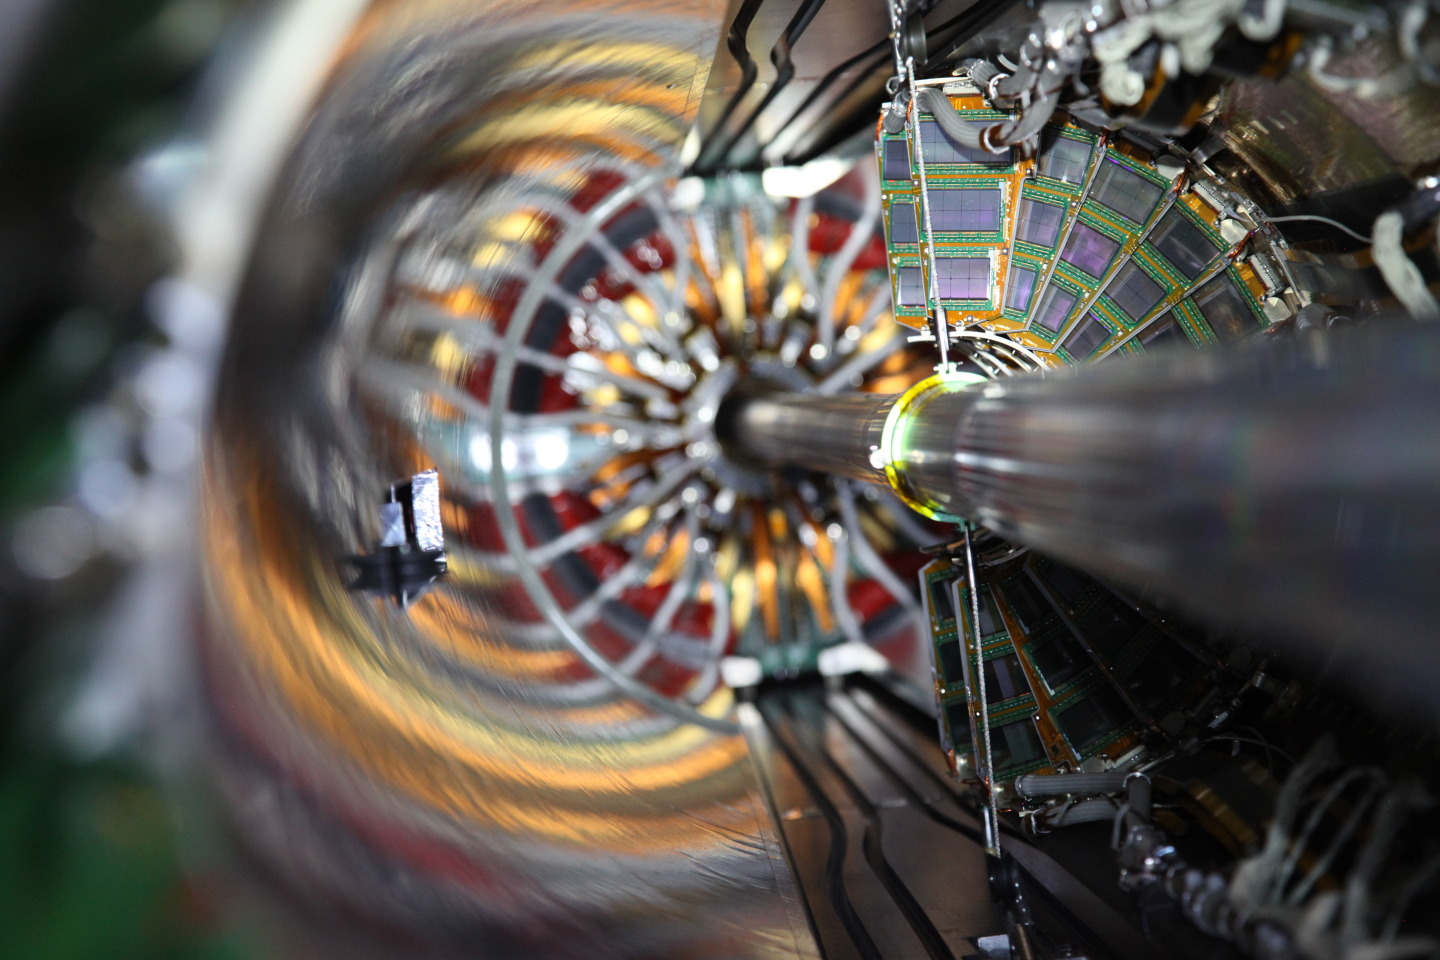
\includegraphics[width=0.45\textwidth,valign=c]{fig/cms/tracker_pixels.jpg}\label{fig:cms_tracker_inner}}\quad
    \subfloat[]{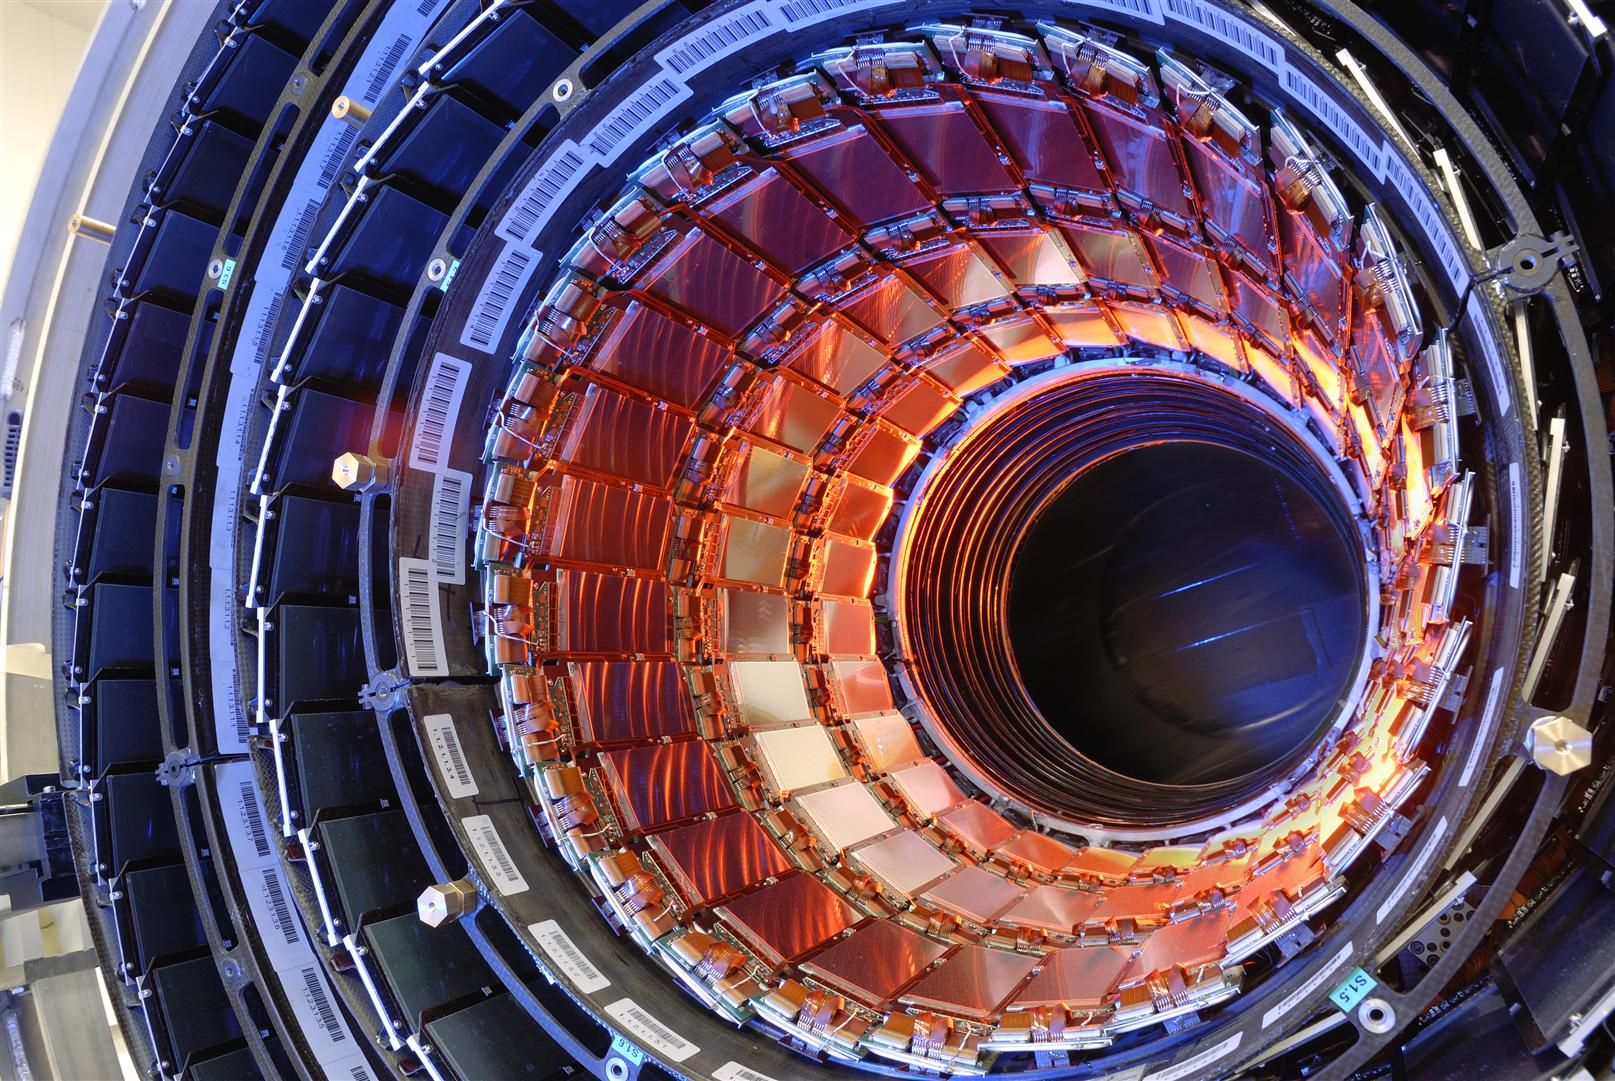
\includegraphics[width=0.45\textwidth,valign=c]{fig/cms/tracker_rainbow.jpg}\label{fig:cms_tracker_outer}}
    \caption{
        A photograph of the inner forward pixel modules (left), from Ref.~\cite{Hoch:2017264}, and the outer barrel layers with a physicist for scale (right), from Ref.~\cite{Maximilien:995912}, of the CMS tracker. 
    }
    \label{fig:cms_tracker_pictures}
\end{figure}

\begin{figure}[htb]
    \centering
    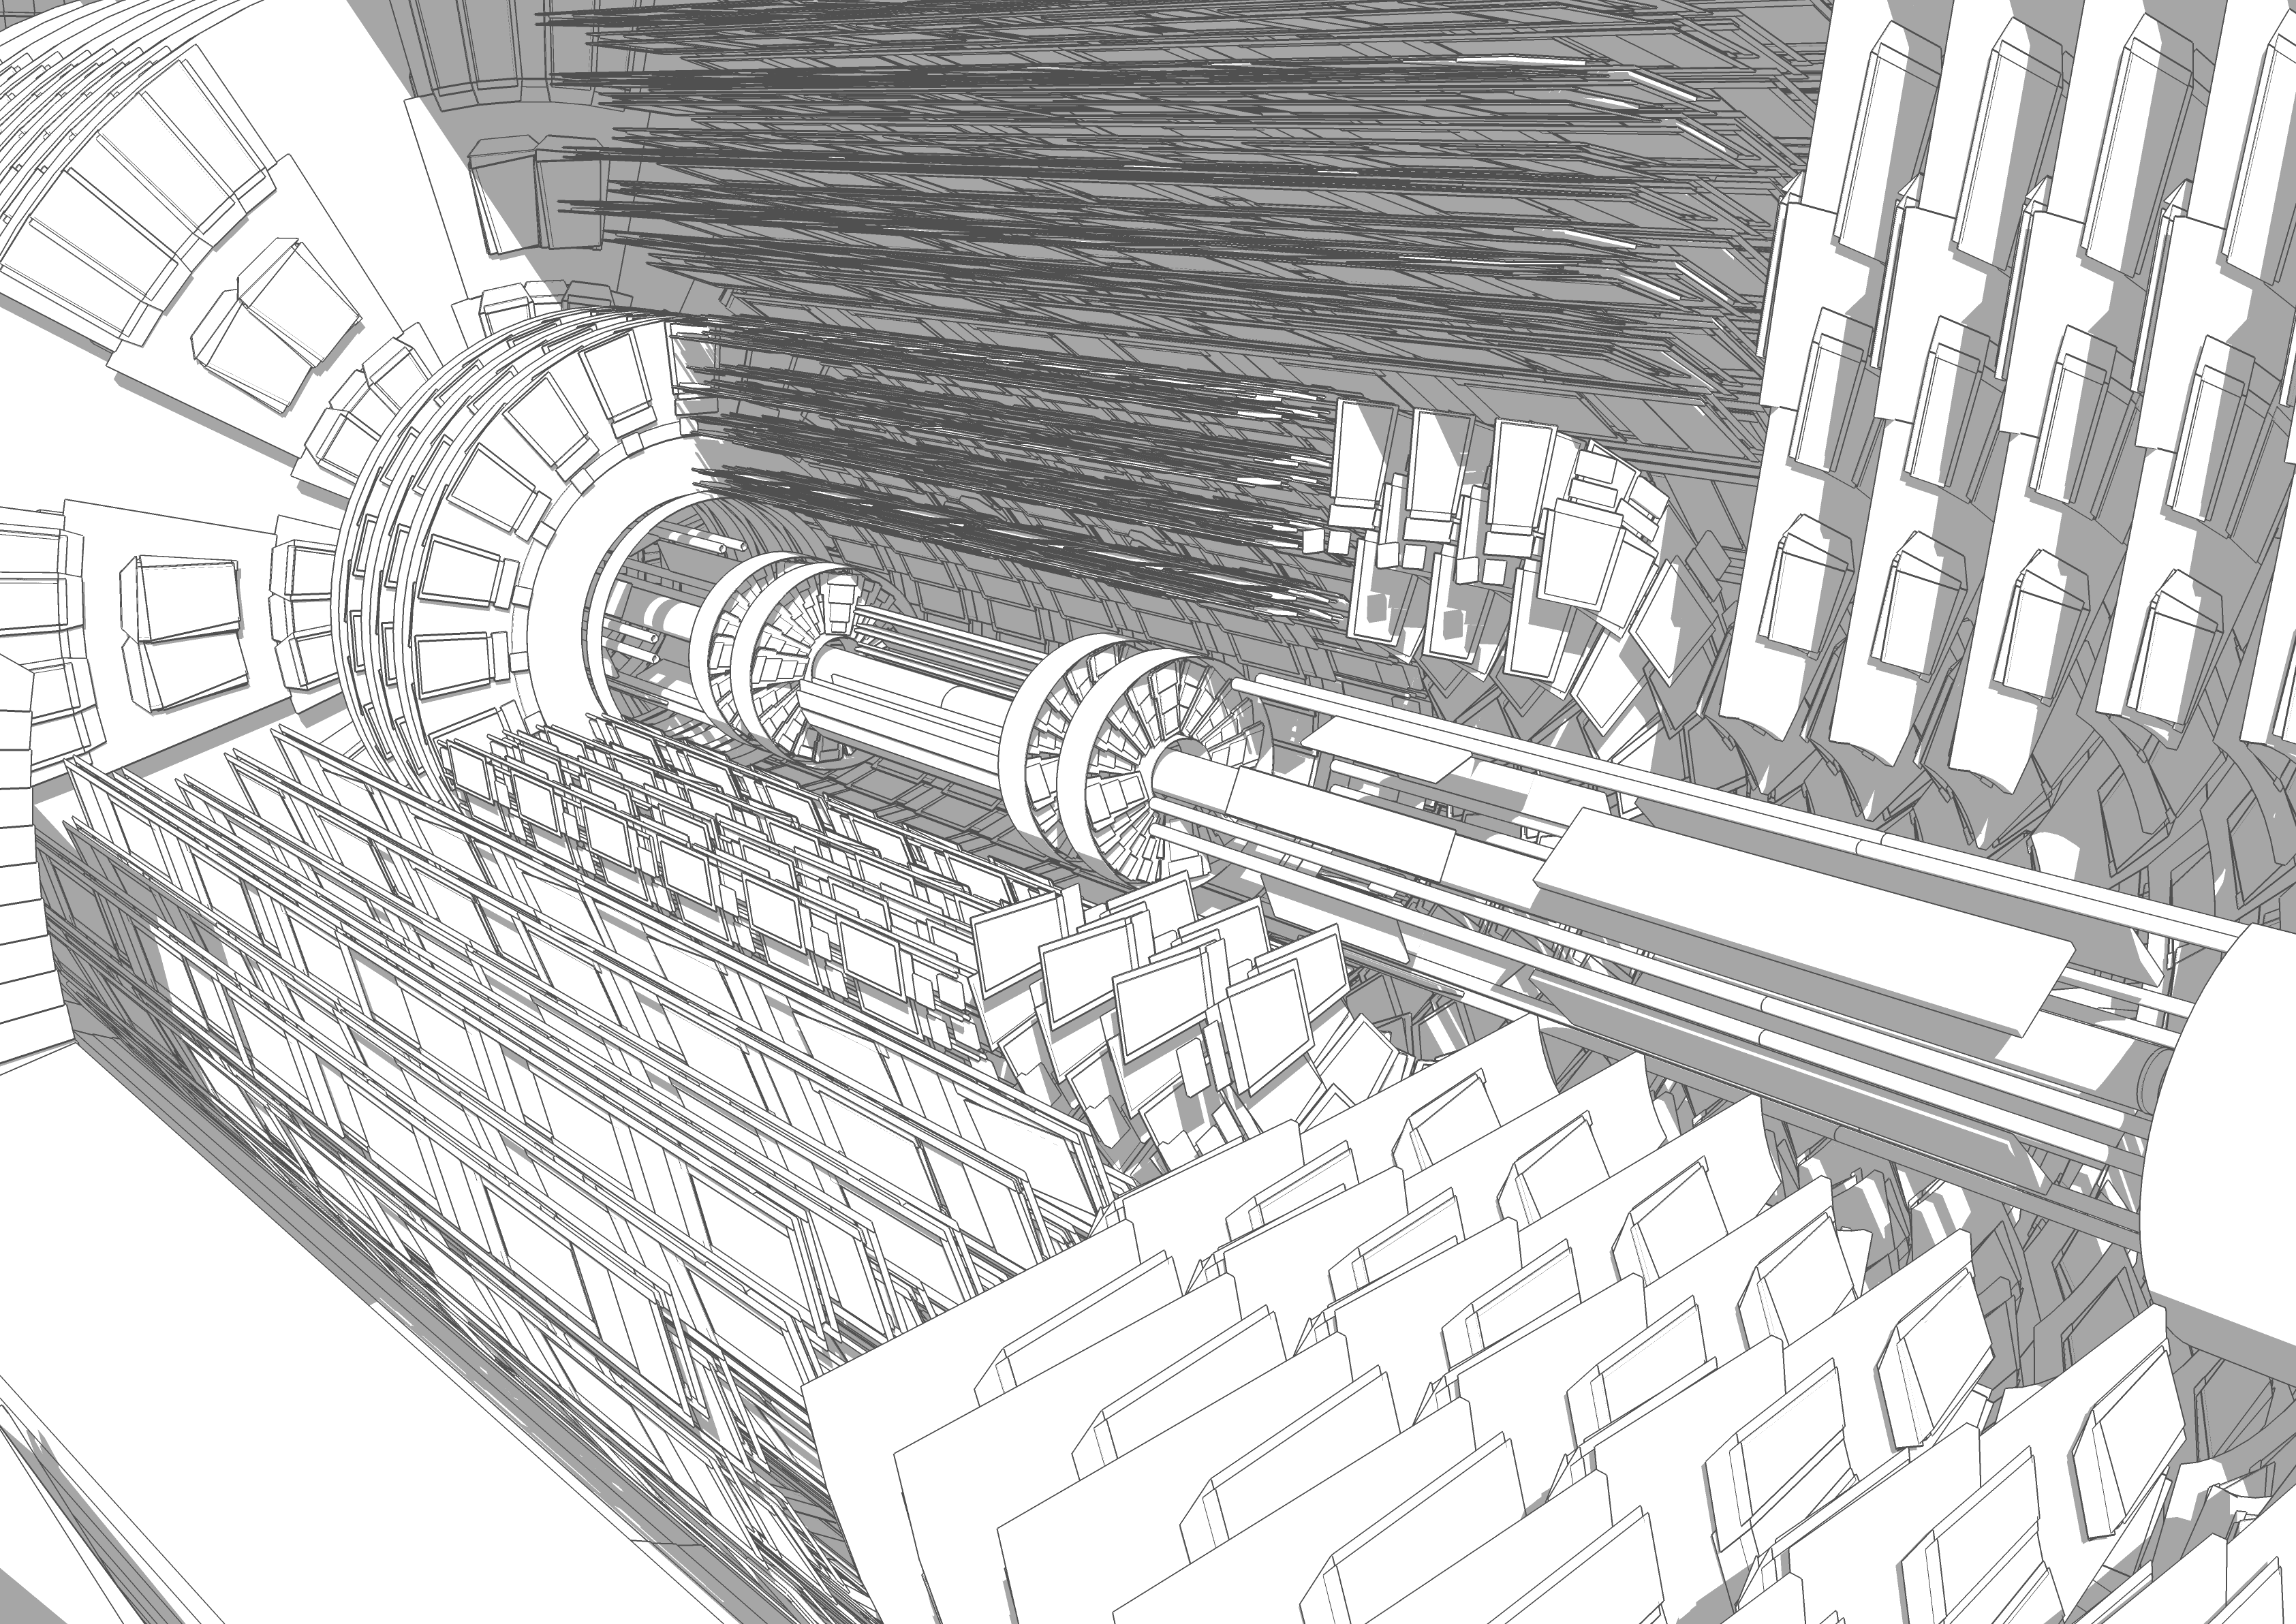
\includegraphics[width=0.9\textwidth,valign=c]{fig/cms/tracker_detailed.png}
    \caption{
        A detailed cutaway diagram of the CMS Phase-1 tracker, from Ref.~\cite{Sakuma:2630160}. 
    }
    \label{fig:cms_tracker_layout}
\end{figure}

\subsection{Electromagnetic calorimeter}
The ECAL (Fig.~\ref{fig:cms_ecal_install}) consists of nearly 80\,000 lead tungstate (PbWO$_4$) crystals\footnotemark{} (Fig.~\ref{fig:cms_ecal_crystal})~\cite{CMSWebECAL}. 
\footnotetext{These crystals were grown in manufacturing plants in Russia and China and took roughly a decade to produce~\cite{CMSWebECAL}.}
When an electron or photon passes through one of these crystals, they interact through the electromagnetic force with the atoms in the crystal lattice, producing a shower of photons. 
This process is called ``scintillation'' and the amount of light produced from one of these interactions is proportional to the energy of the impinging particle. 
Each PbWO$_4$ crystal is glued to a photodetector that collects the scintillation light by the attached crystal and outputs an electric signal proportional to the amount of light collected. 
This signal can then be used to measure the energy of electrons and photons. 

The probability of material interactions ocurring as well as the shape of the shower varies amongst scintillating materials. 
Ultimately, PbWO$_4$ was selected for its short radiation length and small Moli\`ere radius~\cite{CERN-LHCC-97-033}, corresponding to a high probability of interactions and showers localized mostly to a single crystal, respectively. 
The former property is most obviously useful: a high probability of scintillation means electrons and photons are more efficiently collected by the ECAL. 
The latter property, however, is also vital: localized showers are less likely to overlap, so individual particles can be resolved. 

\begin{figure}[htb]
    \centering
    \subfloat[]{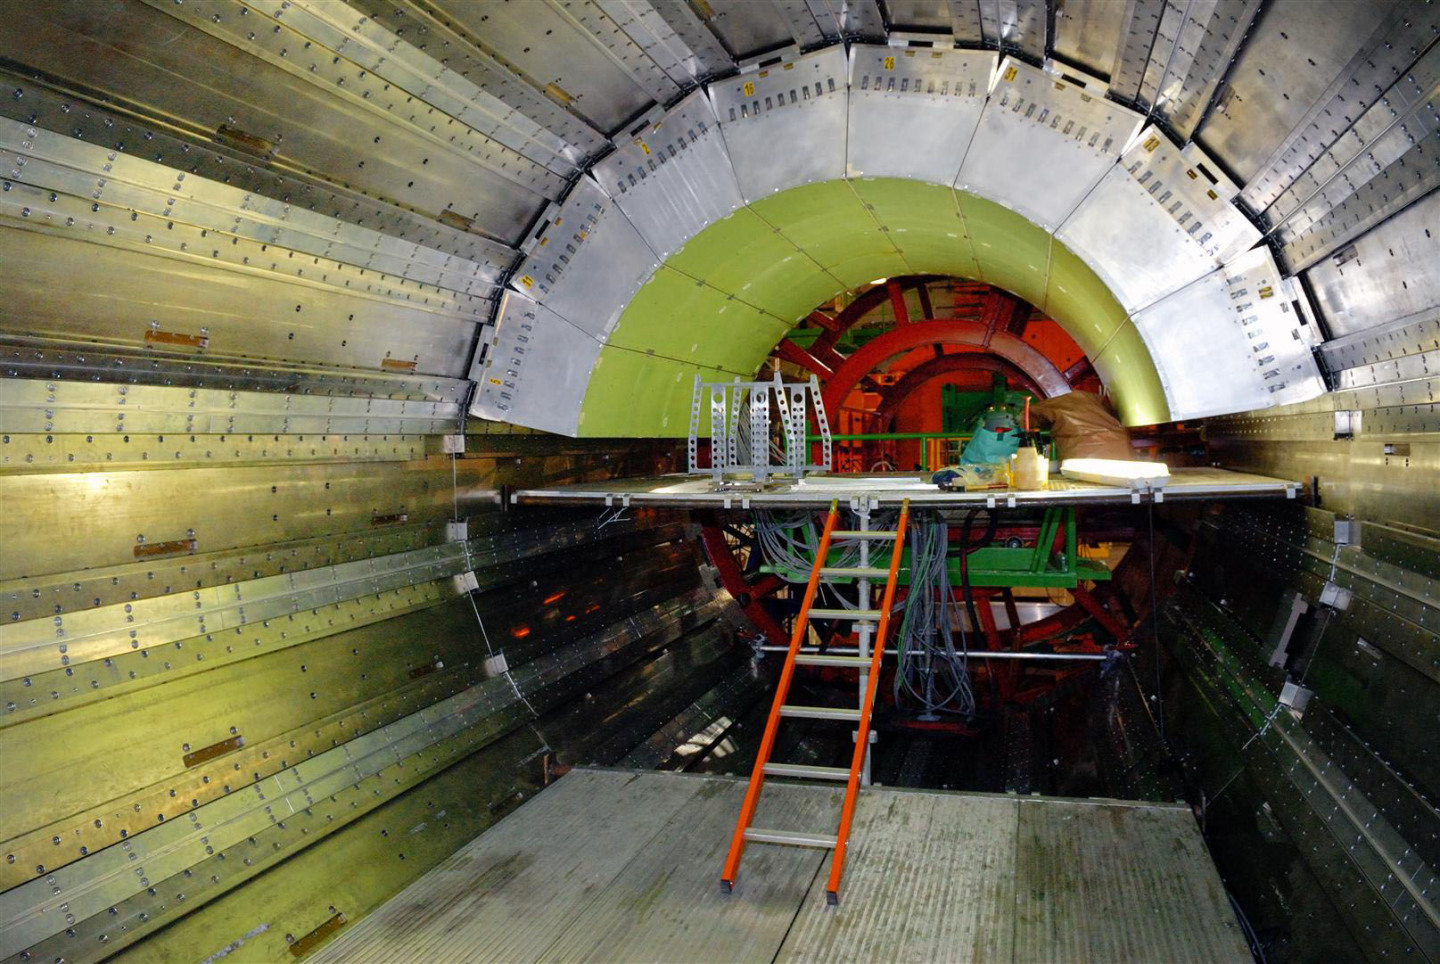
\includegraphics[width=0.45\textwidth,valign=c]{fig/cms/ecal_install.jpg}\label{fig:cms_ecal_install}}\quad
    \subfloat[]{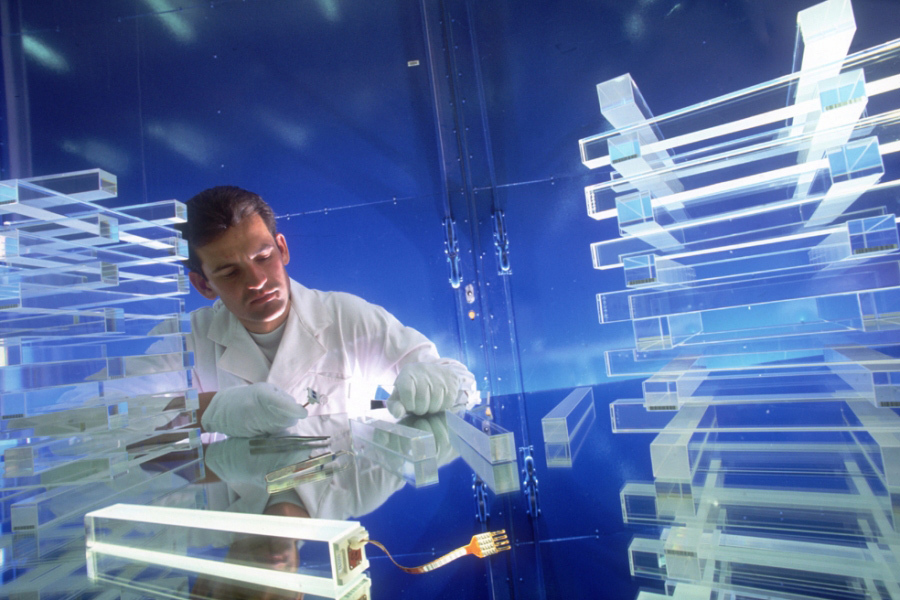
\includegraphics[width=0.45\textwidth,valign=c]{fig/cms/ecal_crystal.jpg}\label{fig:cms_ecal_crystal}}
    \caption{
        A photograph of the CMS electromagnetic calorimeter (ECAL) after half of the modules had been installed (left) and a physicist posed with the lead tungstade scintillator crystals used in the ECAL (right). 
        Both photographs are from Ref.~\cite{Brice:1431477}.
    }
    \label{fig:cms_ecal}
\end{figure}

\subsection{Hadronic calorimeter}
The HCAL (Fig.~\ref{fig:cms_hcal_removed}) is composed of interwoven layers of solid brass or steel plates and plastic scintillator tiles~\cite{CERN-LHCC-97-031}. 
When a hadron interacts with one of the brass and steel ``absorber'' layers, a shower of secondary particles are created. % TODO: add some sort of shower pic, there is one in Kolanoski & Wermes (particle detectors book)
The secondary particles pass through the next scintillator layer, creating scintillation light, then proceed to the next absober layer. 
In this way, large cascading showers of secondary particles are produced according to the energy of the impinging particle, where each scintillator layer gives some measurement, or ``sample,'' of the original particle's energy. 

This kind of calorimeter, which has alternating absorber and scintillator layers, is called a ``sampling'' calorimeter as opposed to a ``homogenous'' calorimeter, wherein a single medium is used to both create the shower and measure the energy. 
Sampling calorimeters are typically less costly and give some information on the shape of the shower, whereas homogenous calorimeters have superior energy resolution. 
In addition, almost all hadronic calorimeters are sampling calorimeters, homogenous hadronic calorimeter would need to be infeasibly large in order to contain a hadronic shower~\cite{KolanoskiWermesDetectors}. 
It is even more critical that the HCAL be compact for CMS, as every increase in size of the inner layers results in large increases in volume of the solenoid and muon chambers, resulting in enormous increases in energy and material costs. 
Due to these space constraints, an additional layer of the HCAL needed to be placed outside of the magnet in order to measure, and absorb, anything that made it past the bulk of the HCAL. 
In fact, the HCAL was already projected to be too costly due to the sheer amount of high-quality brass needed to create the absorber plates. 
To save on costs, the Russian Navy was convinced---without much difficulty---to recycle over one million World War II artillery shells (Fig.~\ref{fig:cms_hcal_russian}), which were designed to withstand large amount of stress (read: explosions) and years at sea, for the cause~\cite{CMSWebHCAL}. 

\begin{figure}[htb]
    \centering
    \subfloat{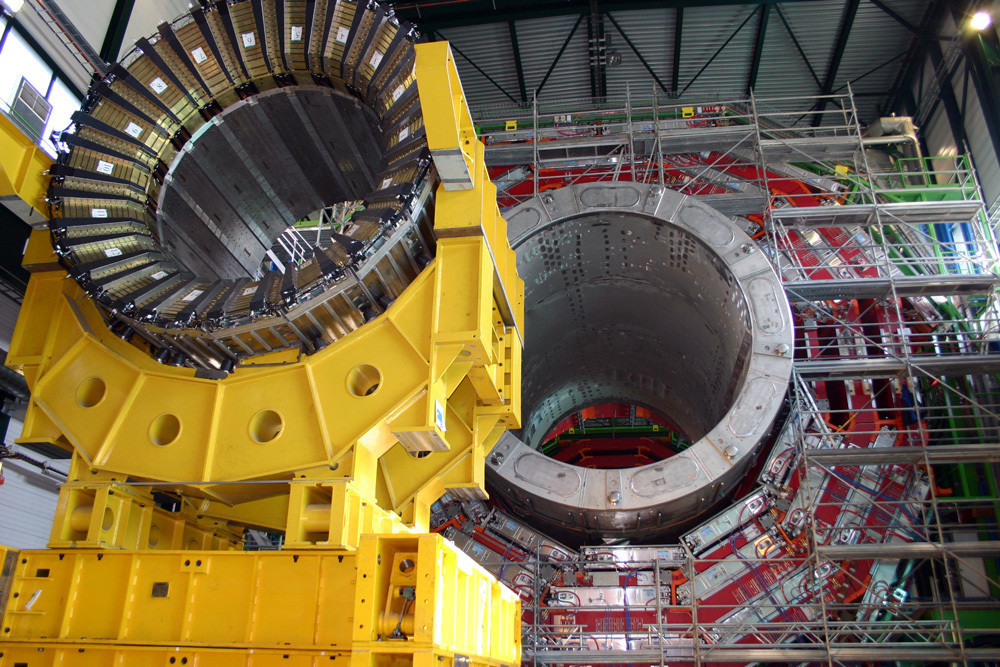
\includegraphics[width=0.45\textwidth,valign=c]{fig/cms/hcal_removed.jpg}\label{fig:cms_hcal_removed}}\quad
    \subfloat{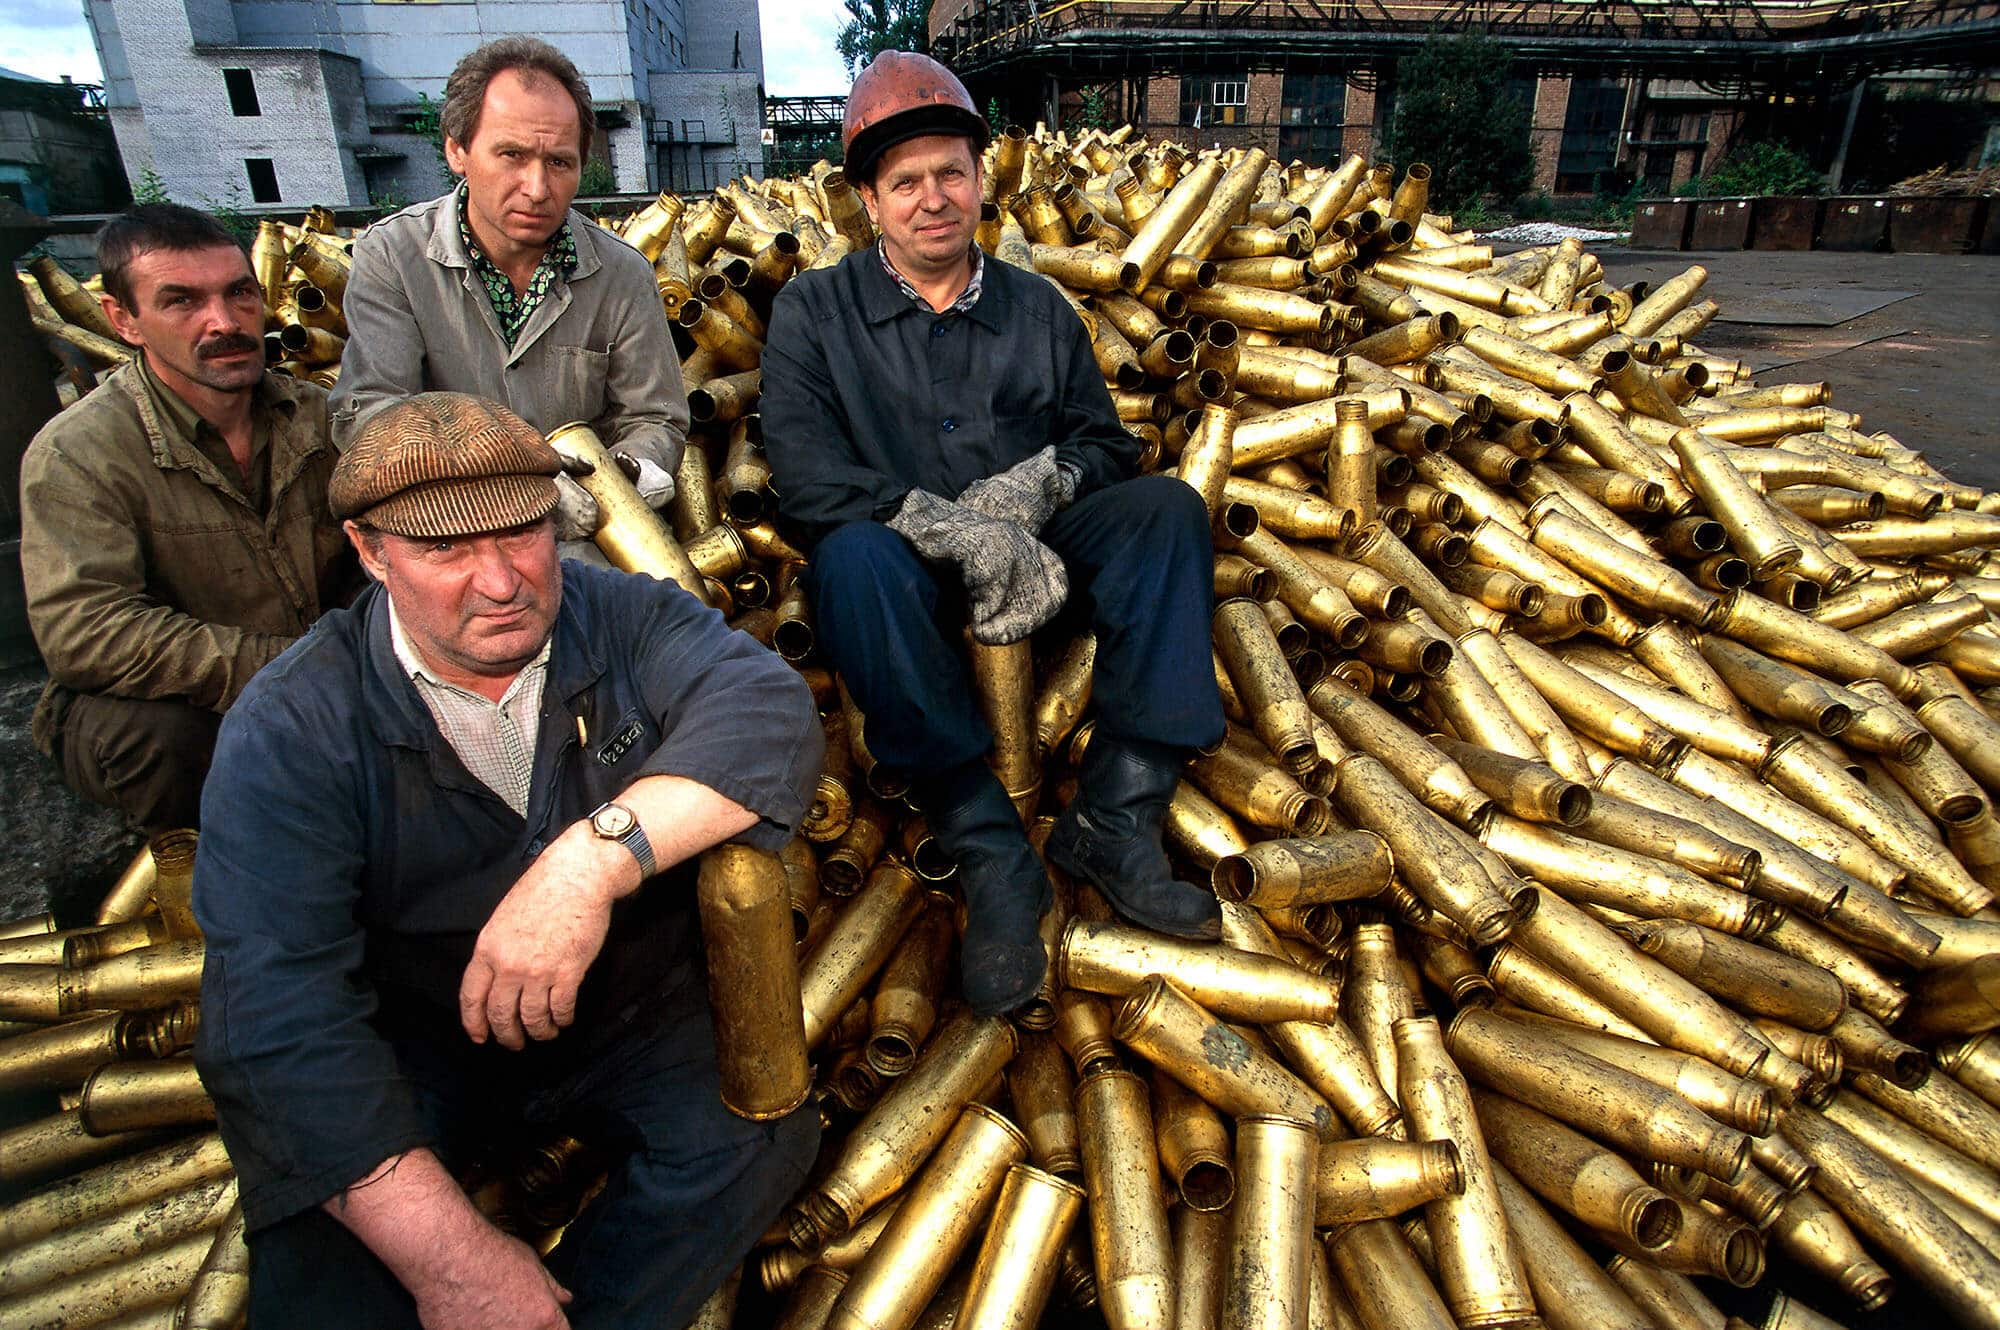
\includegraphics[width=0.45\textwidth,valign=c]{fig/cms/hcal_russian.jpg}\label{fig:cms_hcal_russian}}
    \caption{
        A photograph of the CMS hadronic calorimeter (HCAL) in front of the magnet and muon chambers before the detector was installed in the experiment cavern (left), from Ref.~\cite{Brice:1431485}, and workers in Mormansk sitting on the decomissioned World War II artillery shell casings used to supply the brass for the HCAL (right), from Ref.~\cite{GinterRussianDudes}.
    }
\end{figure}

\subsection{Muon chambers}
The CMS muon system (Fig.~\ref{fig:cms_subdetector_layout}) was originally composed of three different kinds of detectors: drift tubes (DTs) in the barrel, cathode strip chambers (CSCs) in the endcaps, and resistive plate chambers (RPCs) interwoven between the layers of DTs or CSCs. 
All of the different types of muon chambers operate on a similar principle: muons pass through a chamber filled with gas, liberating electrons from the gas atoms; those electrons are then collected on a conductive surface, resulting in an electric signal~\cite{CERN-LHCC-97-032}. 
The DTs (Fig.~\ref{fig:cms_muon_DT}) and CSCs are assembled into multiple layers that serve as an enormous outer tracker (Fig.~\ref{fig:cms_muon_stations}) exclusively for muons. 
DT and CSC modules also both have multiple inner layers in order to give a measurement of a muon's outer track accurate enough to be matched to its inner track in the silicon tracker. 
The RPCs, meanwhile, are designed to give a much faster, if less accurate, measurement of each muon's momentum. 
This measurement can be used to determine whether the pp collision is interesting or not.

\begin{figure}[htb]
    \centering
    \subfloat[]{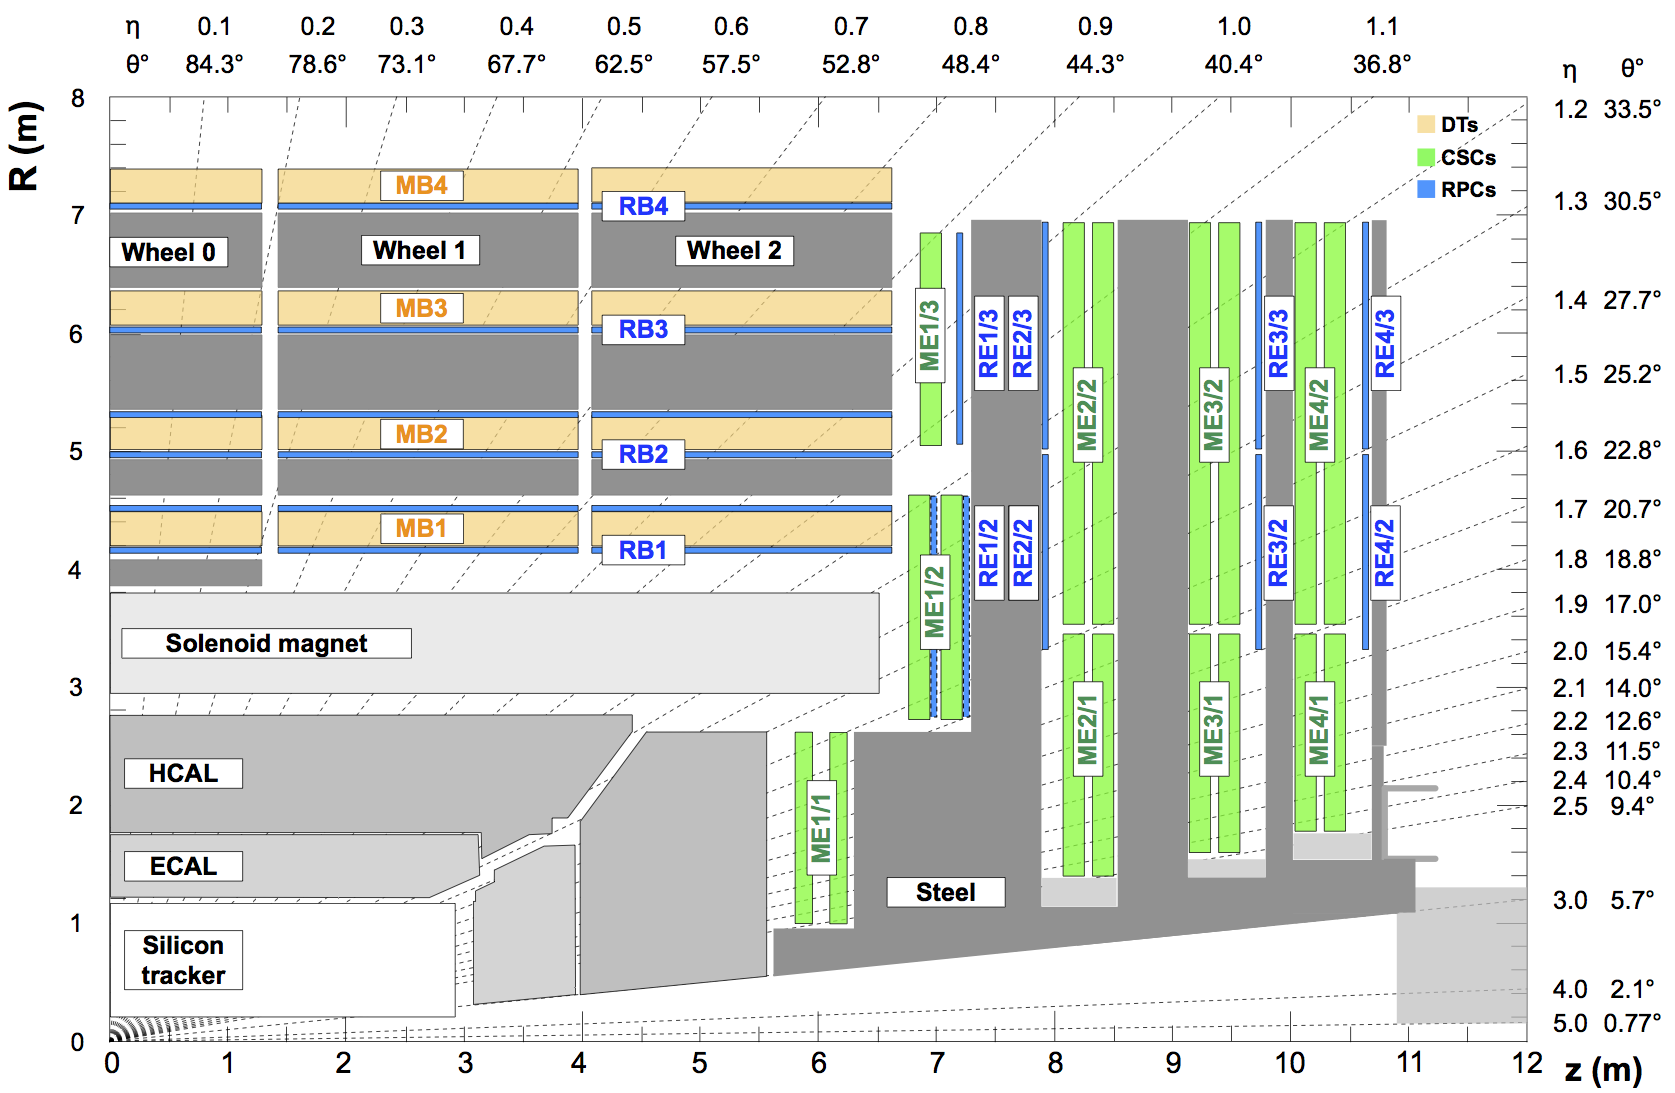
\includegraphics[width=0.6\textwidth,valign=c]{fig/cms/subdetector_layout.png}\label{fig:cms_subdetector_layout}}\quad
    \subfloat[]{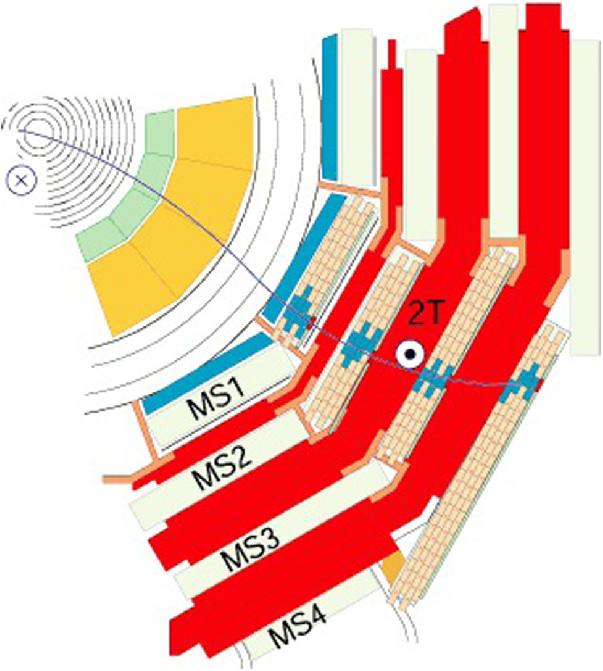
\includegraphics[width=0.3\textwidth,valign=c]{fig/cms/muon_stations.png}\label{fig:cms_muon_stations}}
    \caption{
        The cross section of CMS in the $r$-$z$ plane (left), from Ref.~\cite{CMS:2018rym}, and $r$-$\phi$ plane (right), from Ref.~\cite{CMSWebMuons}. 
        In the $r$-$z$ plane, the DTs, CSCs, and RPCs are drawn in light green, dark green, and blue, respectively, showing the layout of the muon system as well as the other subdetectors. 
        In the $r$-$\phi$ plane, the muon ``stations'' in the barrel are depicted with the DT internals exposed for stations with a throughgoing muon, showing the activation of the individual DT cells (blue) as well as the activiation of a section of the RPC (red).
    }
\end{figure}

\begin{figure}[htb]
    \centering
    \subfloat[]{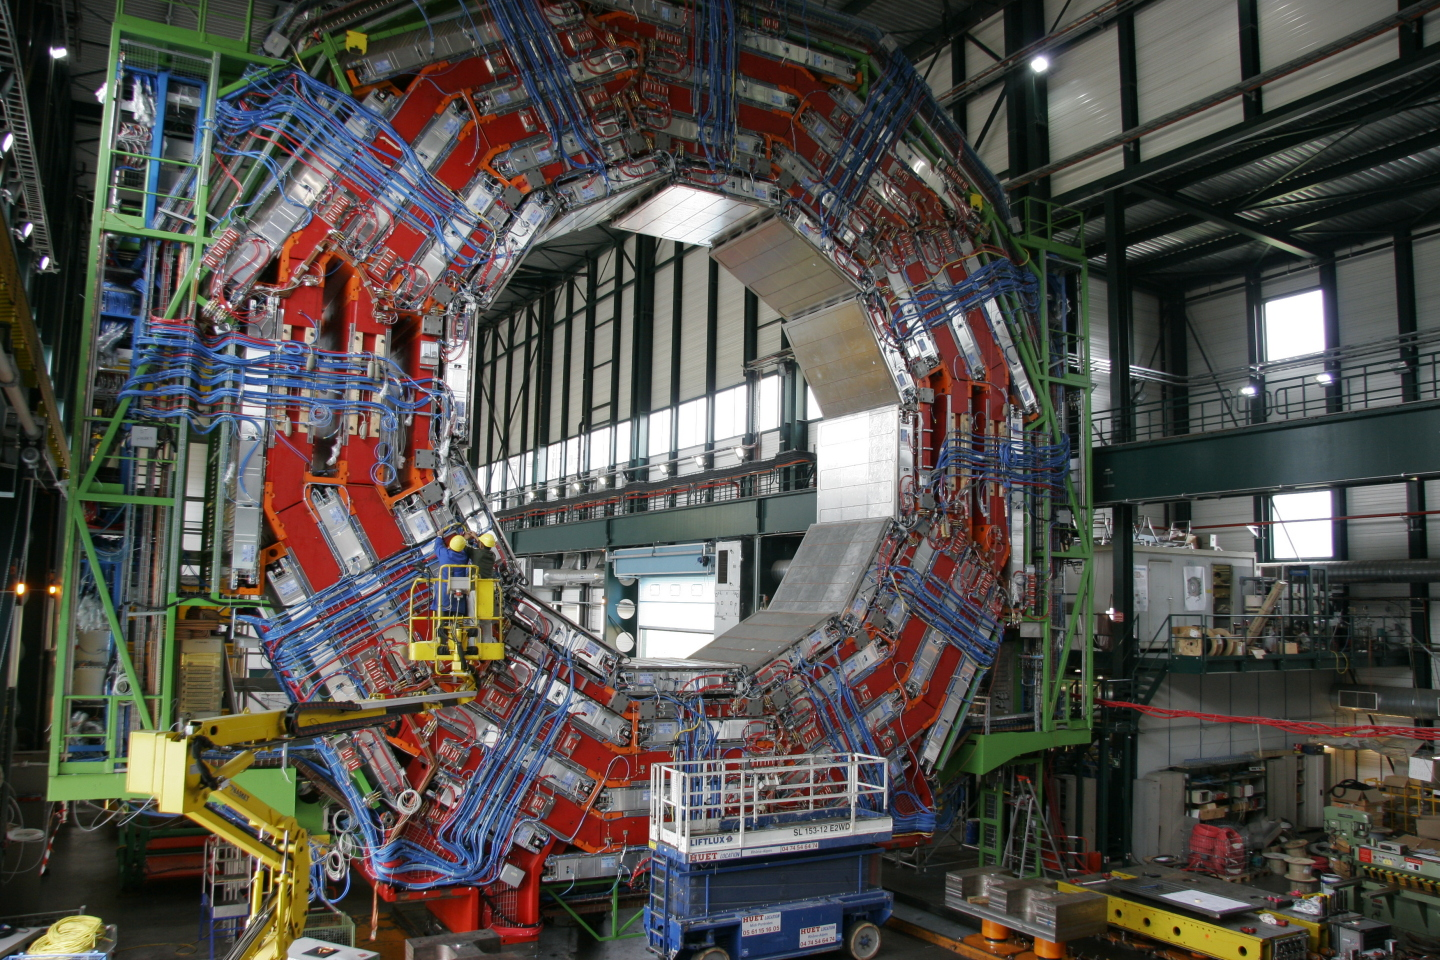
\includegraphics[width=0.465\textwidth,valign=c]{fig/cms/muon_DT_section.jpg}\label{fig:cms_muon_section}}\quad
    \subfloat[]{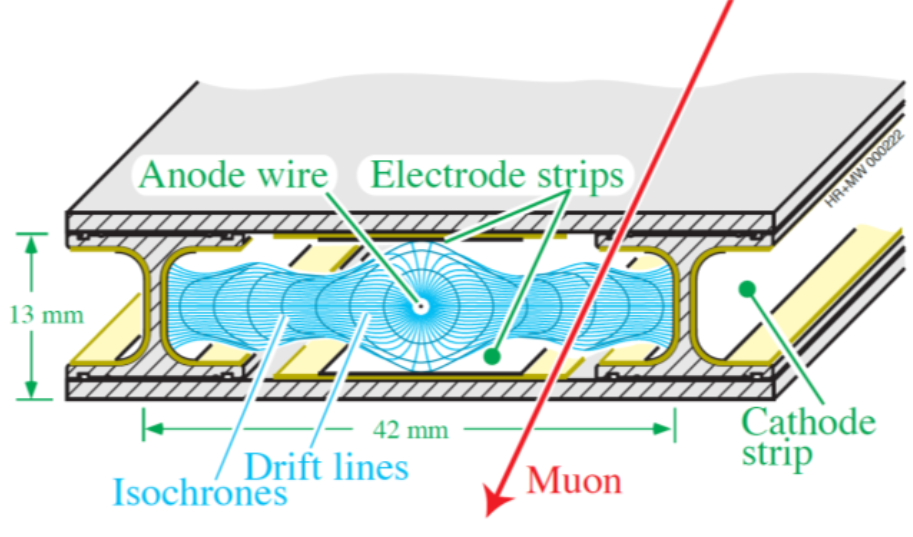
\includegraphics[width=0.435\textwidth,valign=c]{fig/cms/muon_DT_diagram.png}\label{fig:cms_muon_diagram}}
    \caption{
        A photograph of a section of the barrel muon chambers (drift tubes) before they were installed (left), from Ref.~\cite{Hoch:1274451}, and a diagram of a drift tube muon detector (right), from Ref.~\cite{CMSWebMuonDT}. 
    }
    \label{fig:cms_muon_DT}
\end{figure}

\clearpage

\section{The high lumonisity era}
There are three primary knobs to turn at the LHC: what things are being collided, what energy they are collided at, and how many of them are collided at once, or the luminosity. 
Since most of the experiments serviced by the LHC were designed for pp collisions, and because the LHC is designed only for 14\TeV collision energies, the final era of LHC physics will see a massive increase in luminosity. 
That is, at the ``high luminosity'' LHC (HL-LHC), there will be 100--200 concurrent pp collisions per bunch crossing (Fig.~\ref{fig:high_pu}), corresponding to an increase by a factor of 5--7.5.
More collisions means more opportunities for interesting physics. 
For example, in 2017, the LHC produced 3 million Higgs bosons per year, whereas the HL-LHC will produce over 15 million per year~\cite{HighLumiWebFacts}. 

\begin{figure}[htb]
    \centering
    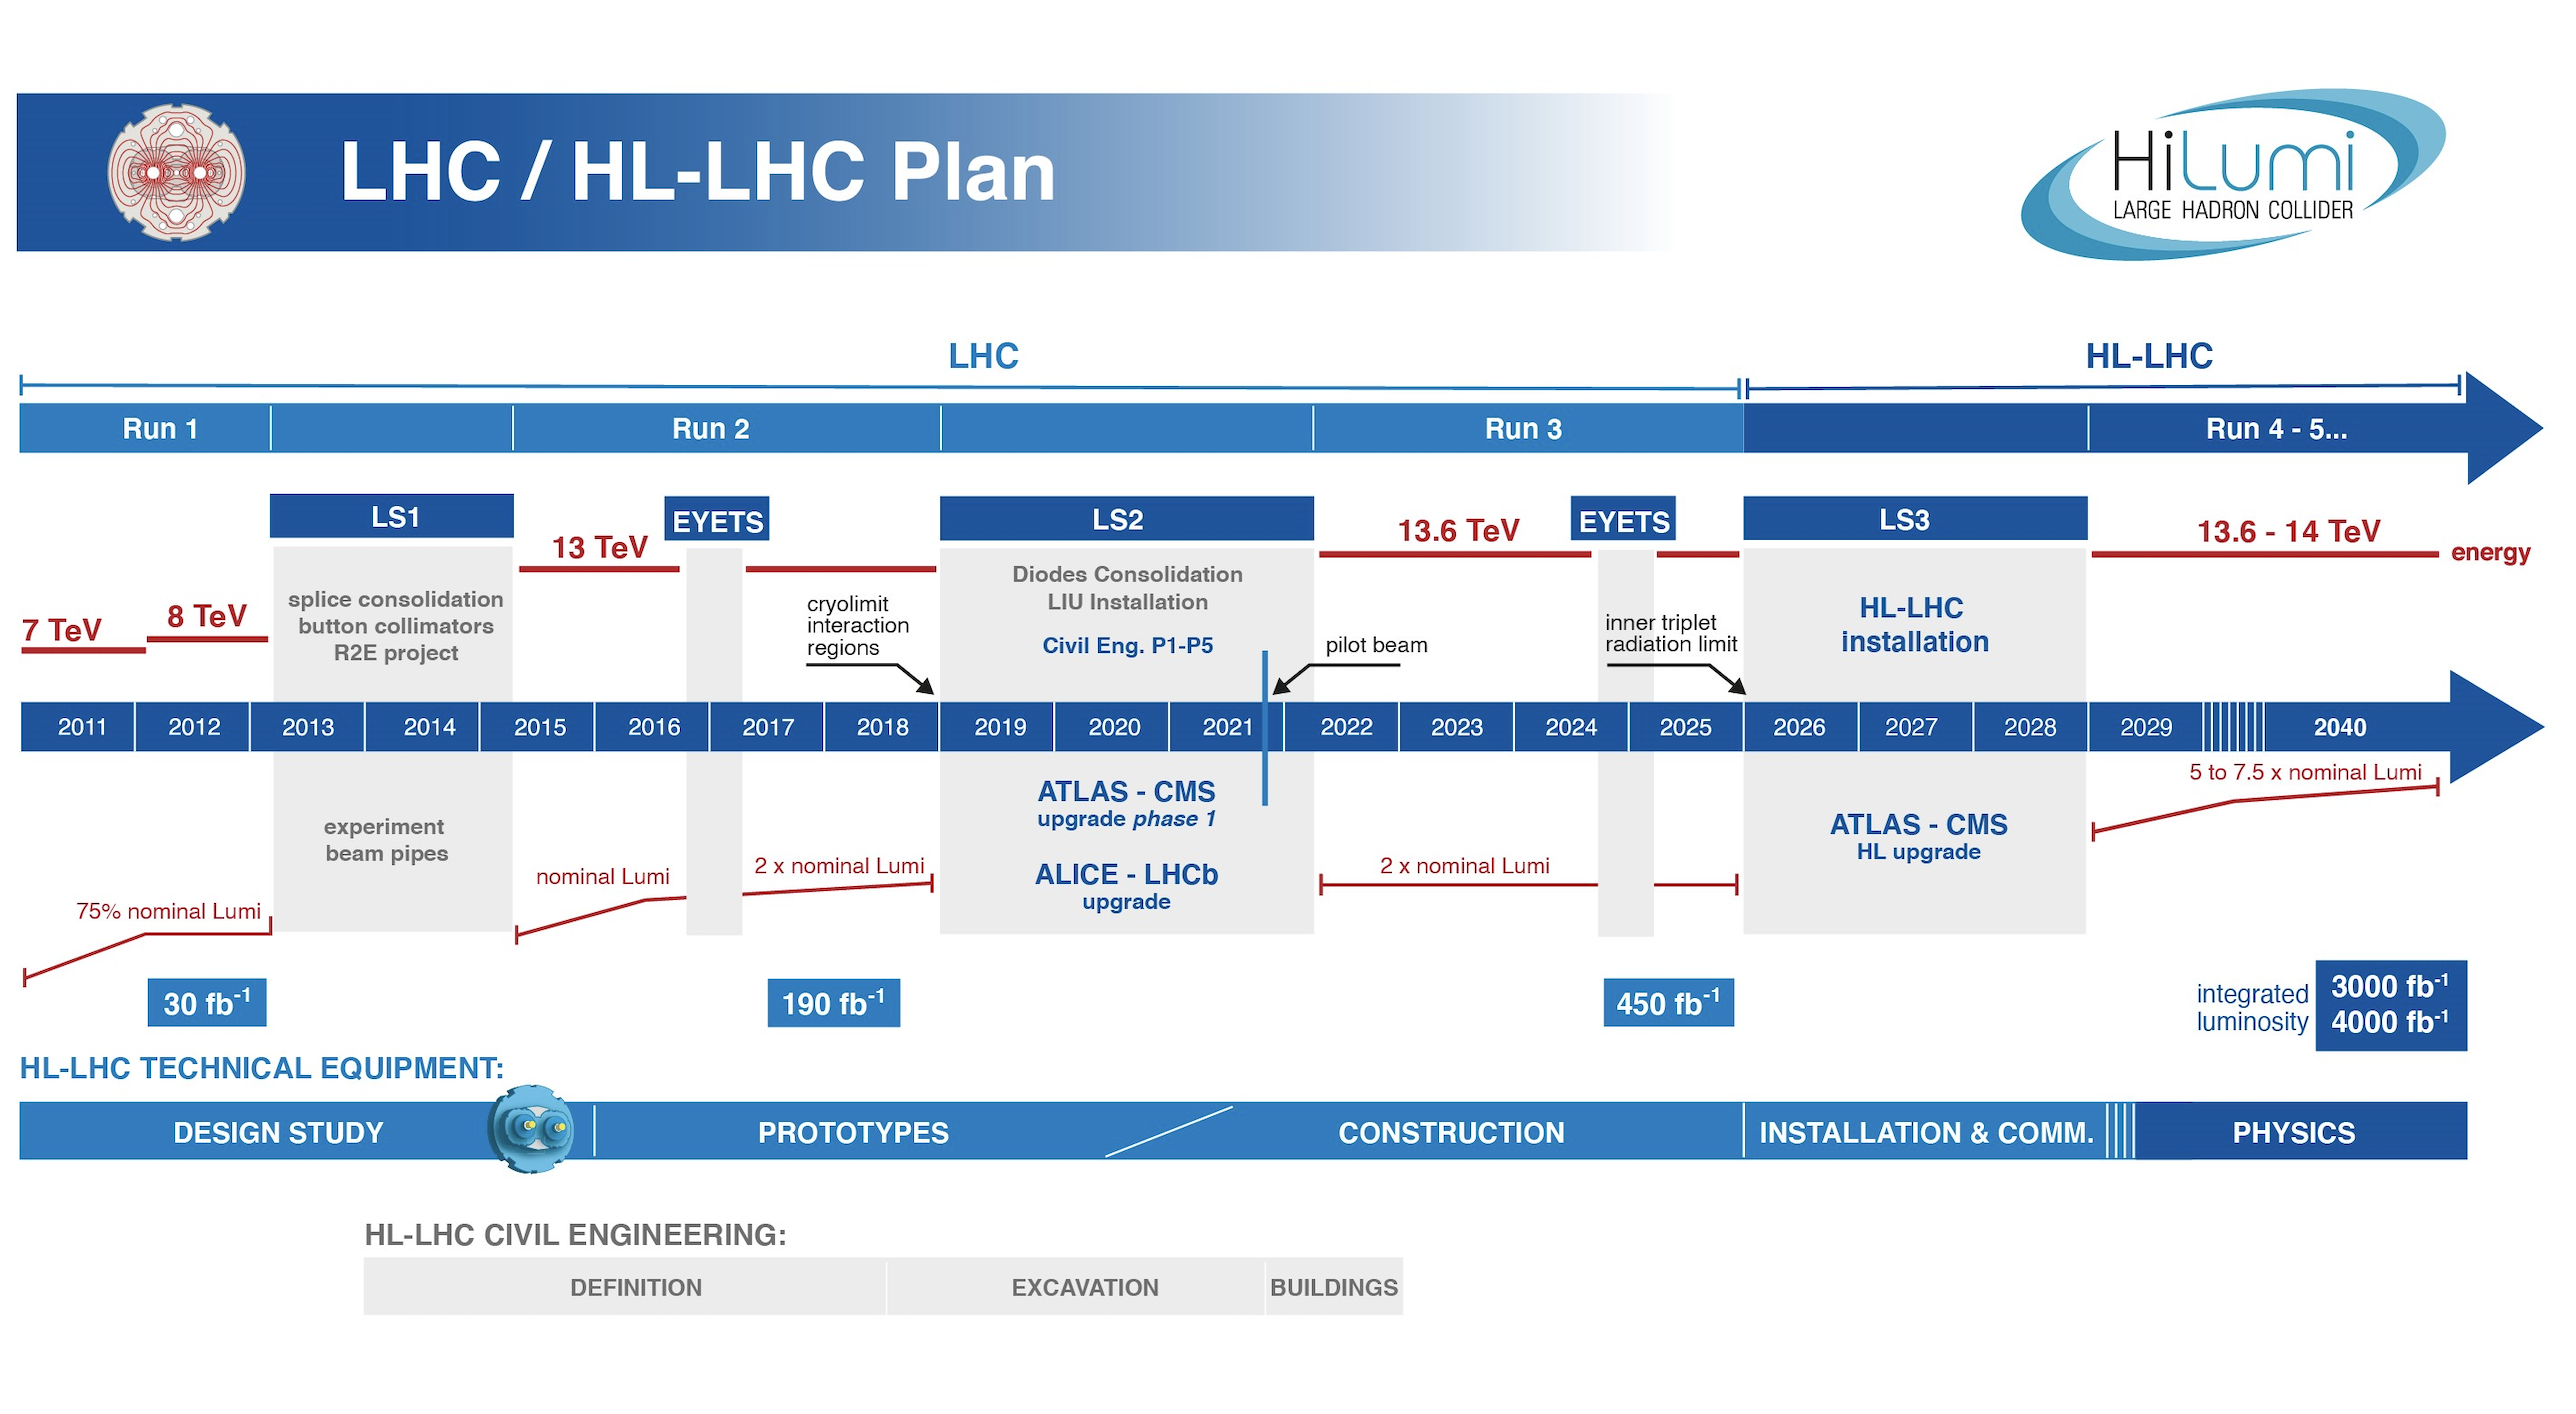
\includegraphics[width=0.9\textwidth,valign=c]{fig/lhc/hl_lhc_timeline.png}
    \caption{
        Lorem ipsum.
    }
    \label{fig:hl_lhc_timeline}
\end{figure}

\begin{figure}[!htb]
    \centering
    \subfloat[]{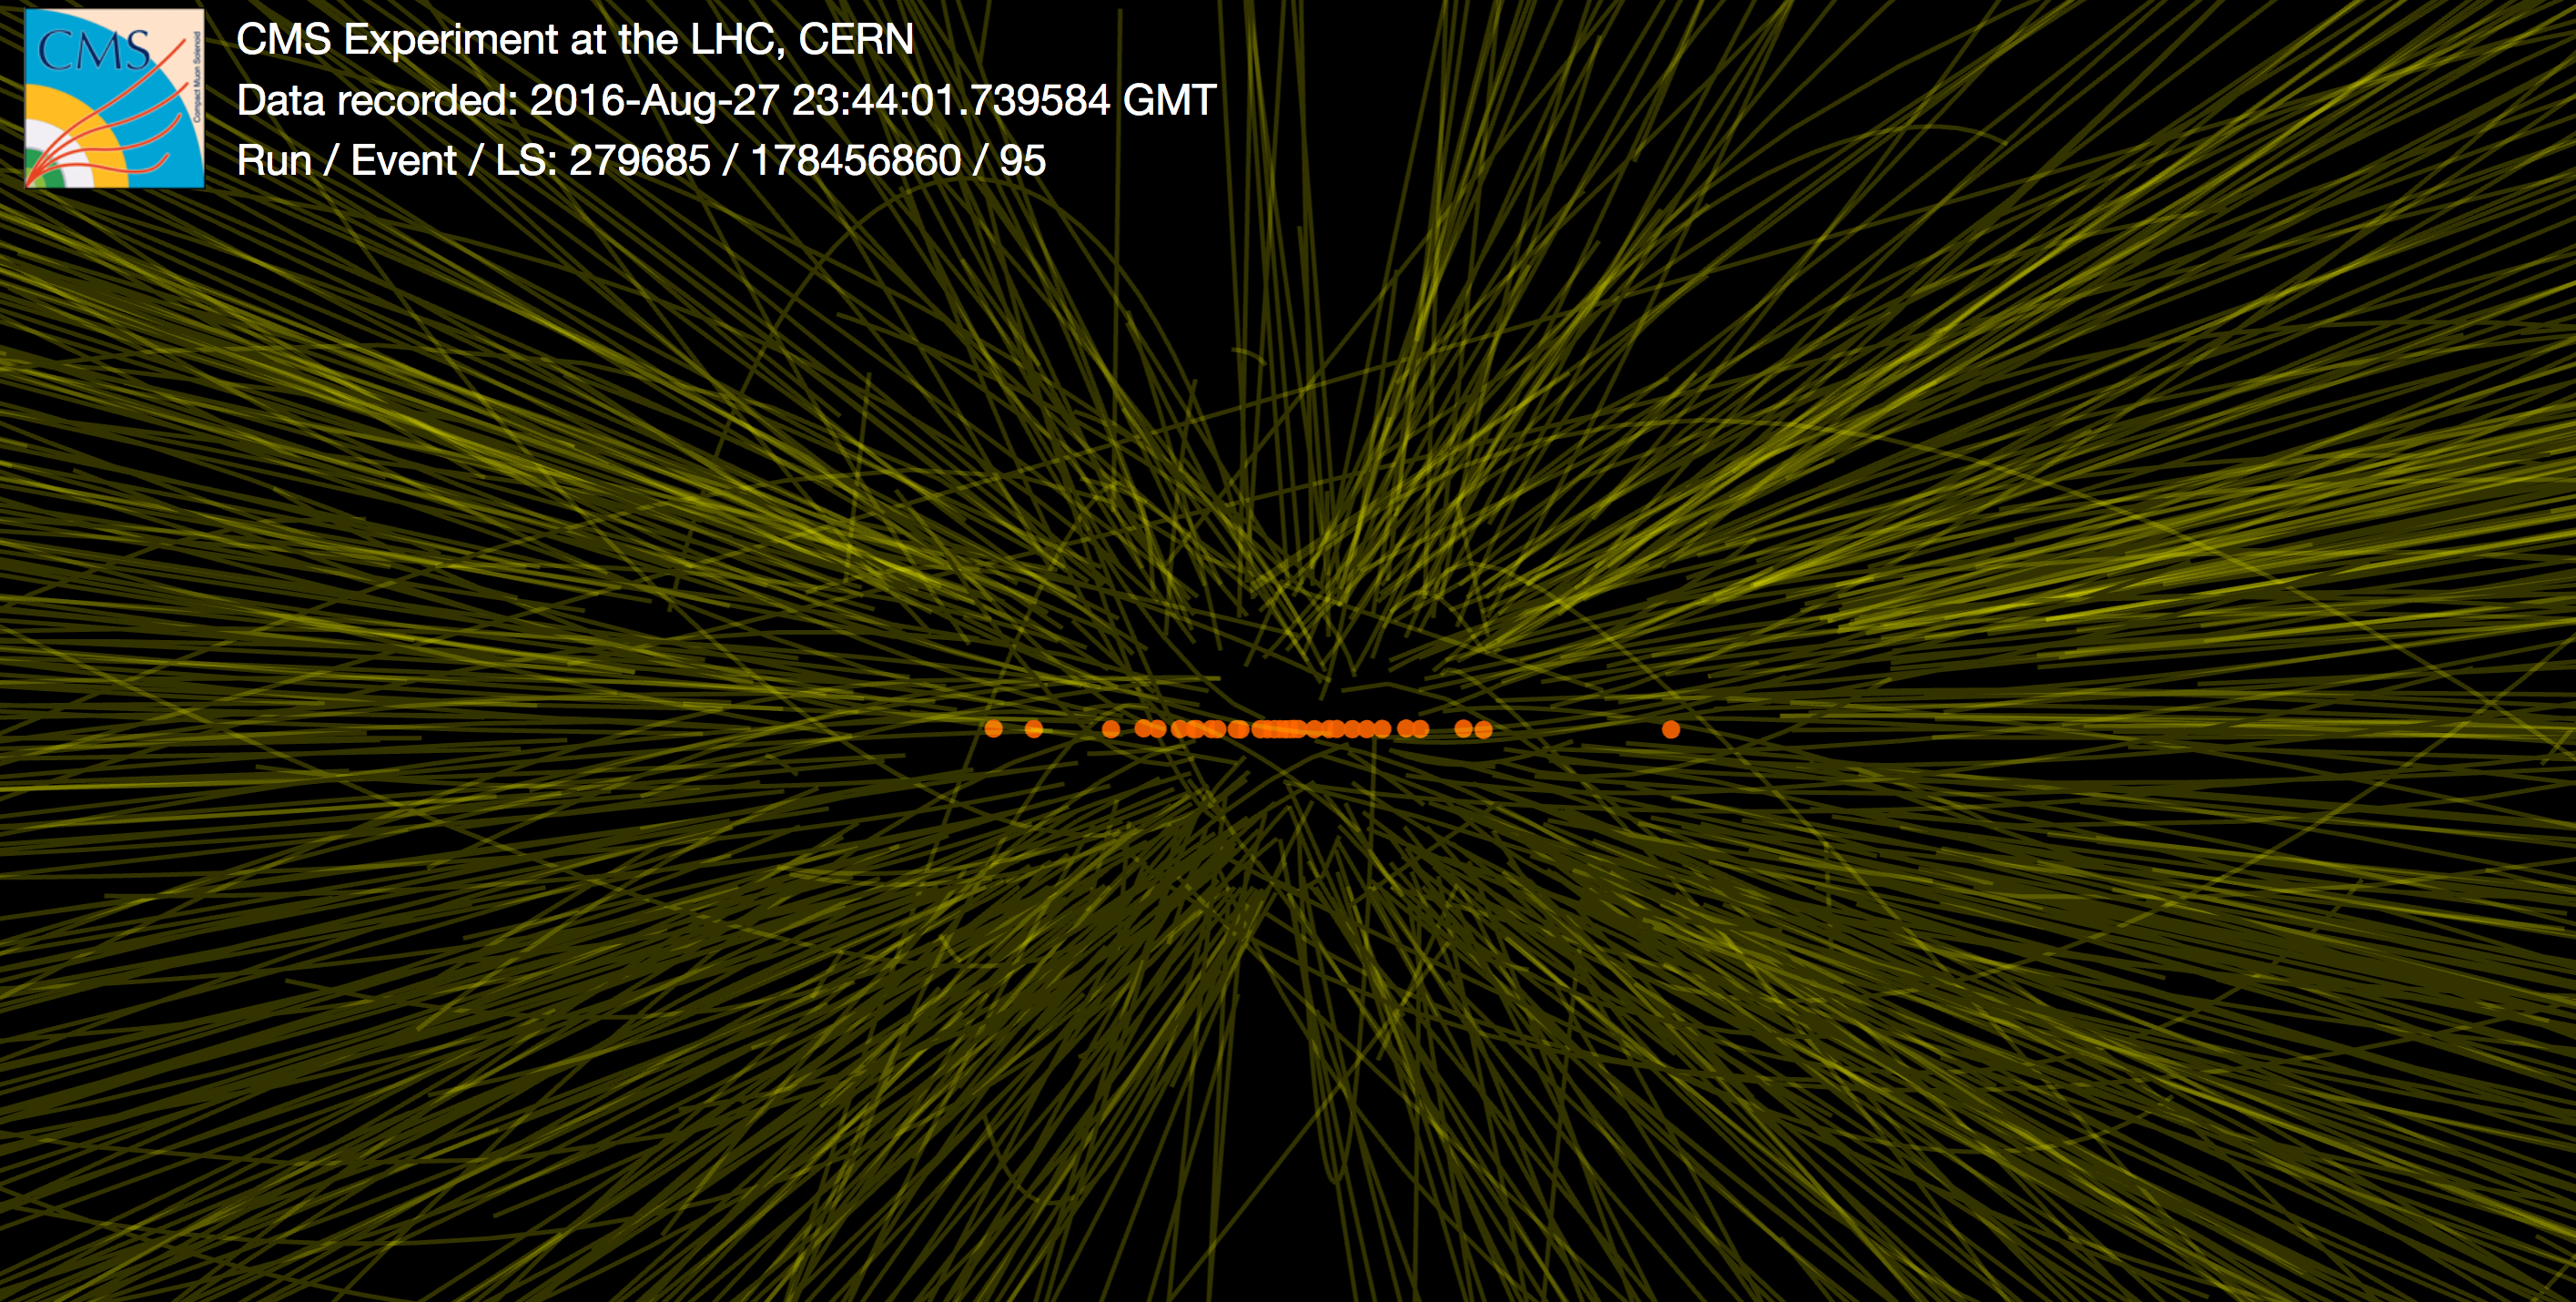
\includegraphics[width=0.45\linewidth]{fig/cms/high_PU_30vtx_side.png}\label{fig:normal_pu}}\qquad
    \subfloat[]{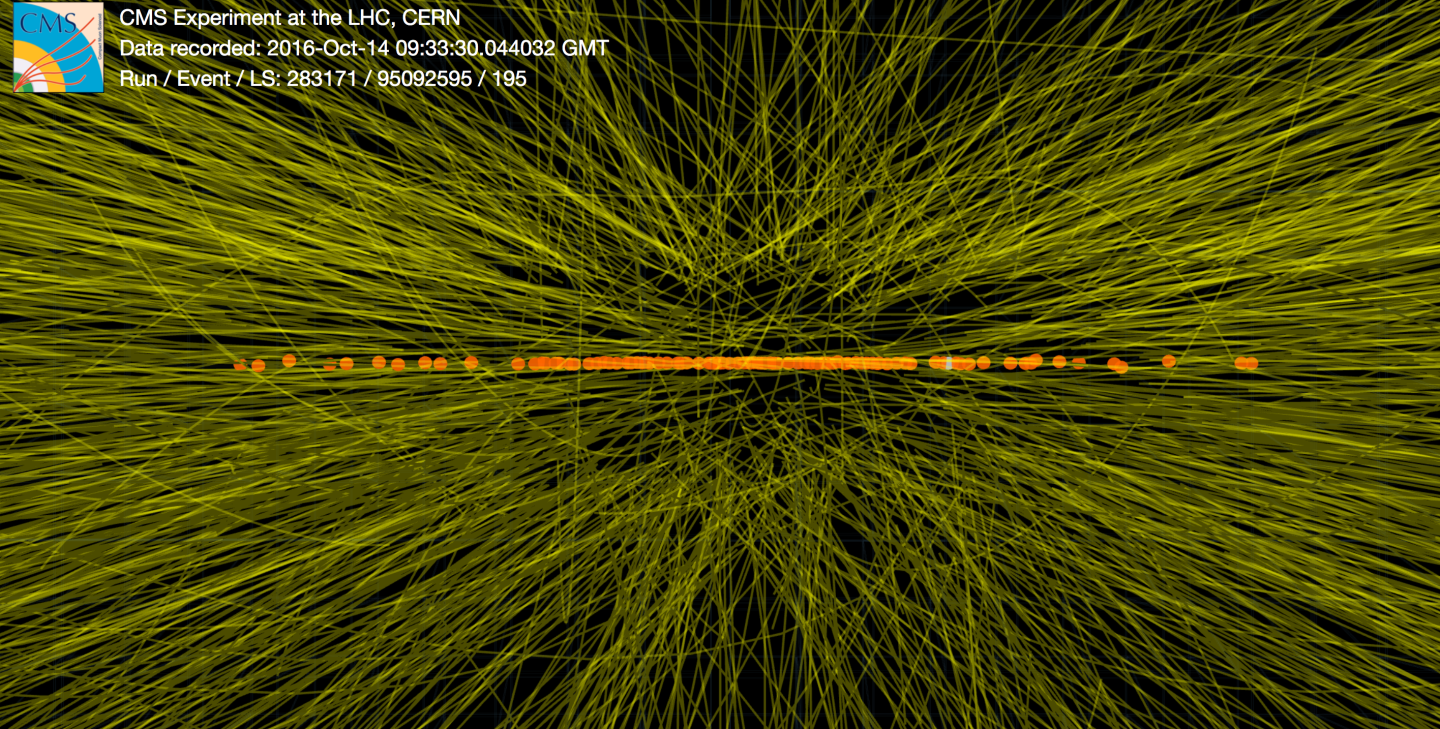
\includegraphics[width=0.45\linewidth]{fig/cms/high_PU_130vtx.png}\label{fig:high_pu}}
    \caption{
        A collision event with standard pileup (a) recorded at CMS in 2016 is shown next to an event with HL-LHC-like pileup (b) recorded at CMS in the same year, from Refs.~\cite{NormalPU2016, HighPU2016}.
        The dots are pp collisions and the thin lines are the reconstructed particle tracks.
    }
    \label{fig:pileup}
\end{figure}

\chapter{Testing the Standard Model}
\begin{aquote}{Stephen Hawking, The Nature of Space and Time, 1996}
    I take the positivist viewpoint that a physical theory is just a mathematical model and that it is meaningless to ask whether it corresponds to reality. 
    All that one can ask is that its predictions should be in agreement with observation. 
\end{aquote}
\section{Vector Boson Scattering}
\section{Search for WH Production via VBS}
\section{Search for VVH Production via VBS}

% Skipping a bunch of chapters
\chapter{A Brighter Tomorrow}
\section{The High Lumonisity LHC}
\section{Line Segment Tracking}
\section{Exascale Data Movement}


% --- Appendices ---
\appendix
\Blinddocument

\chapter{Figures and Such}
This demonstrates how OGS wants figures and tables formatted. For
figures, the caption goes below the figure and ``Figure'' is in bold.
See Figure~\ref{fig:zen}. Tables are formatted with the caption above
the table. See Table~\ref{tab:bad}.

Of course, Table~\ref{tab:bad} looks horrible. It should probably be
formatted like Table~\ref{tab:good} instead.

For facing caption pages, see Table~\ref{tab:facing}. Of course,
facing caption pages are vaguely ridiculous and my implementation of
them in the class file is by far the most brittle part of the
implementation. It's entirely possible that something has changed and
these don't work at all. I implemented it merely for the challenge.

\begin{figure}
\centering
\fbox{\parbox{.9\linewidth}{%
	\noindent
	{\Huge PHD ZEN}\par
	\vskip.5in
	\centerline{comic here}
	\vskip.5in
}}
\caption[``Ph.D. Zen'']{Comic entitled ``Ph.D. Zen'' by Jorge Cham, 2005. Copyright
has not been obtained and so it isn't displayed.}
\label{fig:zen}
\end{figure}

\begin{table}
\centering
\caption[Electronic Dissertation Submission Rates]{Electronic
Dissertation Submission Rates at UCSD, Fall 2005 and Winter 2006.
(First two quarters that the program was available to all Ph.D.
candidates not in a Joint Doctoral Program with SDSU.)}
\label{tab:bad}
\begin{tabular}{|*{5}{>{\centering\arraybackslash}m{.15\linewidth}|}}
\hline
&Ph.D.s awarded (Including Joint degrees) & Electronic submission of
Dissertation & Paper Submission of Dissertation & Percentage of
Electronic Submission\\
\hline
Fall\par 2005 & 84 & 37 & 47 & 44.05\%\\
\hline
Winter\par 2006 & 64 & 42 & 22 & 65.63\%\\
\hline
\end{tabular}
\end{table}

\begin{table}
\centering
\caption[Electronic Dissertation Submission Rates]{Electronic
Dissertation Submission Rates at UCSD, Fall 2005 and Winter 2006.
(First two quarters that the program was available to all Ph.D.
candidates not in a Joint Doctoral Program with SDSU.)}
\label{tab:good}
\renewcommand\tabularxcolumn[1]{>{\RaggedRight\arraybackslash}p{#1}}
\begin{tabularx}{.9\linewidth}{lcccc}
\toprule
&\multicolumn{1}{X}{Ph.D.s awarded (Including Joint degrees)}
&\multicolumn{1}{X}{Electronic submission of Dissertation}
&\multicolumn{1}{X}{Paper Submission of Dissertation}
&\multicolumn{1}{X}{Percentage of Electronic Submission}\\
\midrule
Fall 2005 & 84 & 37 & 47 & 44.05\%\\
Winter 2006 & 64 & 42 & 22 & 65.63\%\\
\bottomrule
\end{tabularx}
\end{table}

\begin{facingcaption}{table}
\caption[UCSD Gender Distribution]{University of
California, San Diego Gender Distribution for the Campus Population,
October~2005\\
(http://assp.ucsd.edu/analytical/Campus\%20Population.shtml)\\
\emph{(This is an example of a facing caption page, the next page is
the example of the table/figure/etc.\ that corresponds to this
caption. It is also an example of table/figure that is rotated 90
degrees to fit the page.)}}
\label{tab:facing}
\renewcommand\tabularxcolumn[1]{>{\RaggedLeft\arraybackslash}p{#1}}
\parindent=0pt
\setbox0=\vbox}
& \multicolumn{1}{c}{\textbf{N}} & \multicolumn{1}{c}{\textbf{\%}}
& \multicolumn{1}{c}{\textbf{N}} & \multicolumn{1}{c}{\textbf{\%}}\\
\midrule
Students & 12,987 & 51\% & 12,686 & 49\% & 25,673 & 100\%\\
Employees & 9,943 & 56\% &  7,671 & 44\% & 17,614 & 100\%\\
\addlinespace
\hfill\textbf{Total} & \textbf{22,930} & \textbf{53\%} &
\textbf{20,357} & \textbf{47\%} & \textbf{43,287} & \textbf{100\%}\\
\bottomrule
\end{tabularx}
\singlespacing

\emph{Notes}:
\begin{enumerate}
\item The counts shown below will differ from the official quarterly
Registrar's registration report because 1) data for residents in the
Schools of Medicine and Pharmacy and Pharmaceutical Science are
excluded, and 2) registered, non-matriculated, visiting students are
included.
\item Student workers are excluded from employees; however emeritus
faculty and others on recall status are included.
\end{enumerate}

Campus Planning. Analytical Studies and Space Planning\\
31 January 2006
}
\centerline{\rotatebox{90}{\box0}}
\end{facingcaption}

% This will give us some more text
\Blinddocument

% Skipping a bunch of chapters
\chapter{Another chapter}
\begin{figure}
\centering
\fbox{\hbox to.8\linewidth{\hss Another figure\hss}}
\caption{Another figure caption}
\end{figure}
\begin{table}
\centering
\caption{Another table caption}
\begin{tabular}{ccc}
\toprule
X&Y&Z\\
\midrule
a&b&c\\
\bottomrule
\end{tabular}
\end{table}
\begin{figure}
\caption{ASDF fig}
\end{figure}
\begin{table}
\caption{ASDF tab}
\end{table}


% Stuff at the end of the dissertation goes in the back matter
\backmatter
\bibliographystyle{plain} % Or whatever style you want like plainnat
\bibliography{references}

\end{document}
